\documentclass[twoside]{book}

% Packages required by doxygen
\usepackage{calc}
\usepackage{doxygen}
\usepackage{graphicx}
\usepackage[utf8]{inputenc}
\usepackage{makeidx}
\usepackage{multicol}
\usepackage{multirow}
\usepackage{textcomp}
\usepackage[table]{xcolor}

% Font selection
\usepackage[T1]{fontenc}
\usepackage{mathptmx}
\usepackage[scaled=.90]{helvet}
\usepackage{courier}
\usepackage{amssymb}
\usepackage{sectsty}
\renewcommand{\familydefault}{\sfdefault}
\allsectionsfont{%
  \fontseries{bc}\selectfont%
  \color{darkgray}%
}
\renewcommand{\DoxyLabelFont}{%
  \fontseries{bc}\selectfont%
  \color{darkgray}%
}

% Page & text layout
\usepackage{geometry}
\geometry{%
  a4paper,%
  top=2.5cm,%
  bottom=2.5cm,%
  left=2.5cm,%
  right=2.5cm%
}
\tolerance=750
\hfuzz=15pt
\hbadness=750
\setlength{\emergencystretch}{15pt}
\setlength{\parindent}{0cm}
\setlength{\parskip}{0.2cm}
\makeatletter
\renewcommand{\paragraph}{%
  \@startsection{paragraph}{4}{0ex}{-1.0ex}{1.0ex}{%
    \normalfont\normalsize\bfseries\SS@parafont%
  }%
}
\renewcommand{\subparagraph}{%
  \@startsection{subparagraph}{5}{0ex}{-1.0ex}{1.0ex}{%
    \normalfont\normalsize\bfseries\SS@subparafont%
  }%
}
\makeatother

% Headers & footers
\usepackage{fancyhdr}
\pagestyle{fancyplain}
\fancyhead[LE]{\fancyplain{}{\bfseries\thepage}}
\fancyhead[CE]{\fancyplain{}{}}
\fancyhead[RE]{\fancyplain{}{\bfseries\leftmark}}
\fancyhead[LO]{\fancyplain{}{\bfseries\rightmark}}
\fancyhead[CO]{\fancyplain{}{}}
\fancyhead[RO]{\fancyplain{}{\bfseries\thepage}}
\fancyfoot[LE]{\fancyplain{}{}}
\fancyfoot[CE]{\fancyplain{}{}}
\fancyfoot[RE]{\fancyplain{}{\bfseries\scriptsize Generated on Mon Jun 30 2014 17\-:03\-:34 for Asylia by Doxygen }}
\fancyfoot[LO]{\fancyplain{}{\bfseries\scriptsize Generated on Mon Jun 30 2014 17\-:03\-:34 for Asylia by Doxygen }}
\fancyfoot[CO]{\fancyplain{}{}}
\fancyfoot[RO]{\fancyplain{}{}}
\renewcommand{\footrulewidth}{0.4pt}
\renewcommand{\chaptermark}[1]{%
  \markboth{#1}{}%
}
\renewcommand{\sectionmark}[1]{%
  \markright{\thesection\ #1}%
}

% Indices & bibliography
\usepackage{natbib}
\usepackage[titles]{tocloft}
\setcounter{tocdepth}{3}
\setcounter{secnumdepth}{5}
\makeindex

% Hyperlinks (required, but should be loaded last)
\usepackage{ifpdf}
\ifpdf
  \usepackage[pdftex,pagebackref=true]{hyperref}
\else
  \usepackage[ps2pdf,pagebackref=true]{hyperref}
\fi
\hypersetup{%
  colorlinks=true,%
  linkcolor=blue,%
  citecolor=blue,%
  unicode%
}

% Custom commands
\newcommand{\clearemptydoublepage}{%
  \newpage{\pagestyle{empty}\cleardoublepage}%
}


%===== C O N T E N T S =====

\begin{document}

% Titlepage & ToC
\hypersetup{pageanchor=false}
\pagenumbering{roman}
\begin{titlepage}
\vspace*{7cm}
\begin{center}%
{\Large Asylia }\\
\vspace*{1cm}
{\large Generated by Doxygen 1.8.6}\\
\vspace*{0.5cm}
{\small Mon Jun 30 2014 17:03:34}\\
\end{center}
\end{titlepage}
\clearemptydoublepage
\tableofcontents
\clearemptydoublepage
\pagenumbering{arabic}
\hypersetup{pageanchor=true}

%--- Begin generated contents ---
\chapter{Hierarchical Index}
\section{Class Hierarchy}
This inheritance list is sorted roughly, but not completely, alphabetically\-:\begin{DoxyCompactList}
\item \contentsline{section}{Activity}{\pageref{classActivity}}{}
\begin{DoxyCompactList}
\item \contentsline{section}{Battle\-Activity}{\pageref{classBattleActivity}}{}
\item \contentsline{section}{End\-Activity}{\pageref{classEndActivity}}{}
\item \contentsline{section}{Equip\-Activity}{\pageref{classEquipActivity}}{}
\item \contentsline{section}{Item\-Activity}{\pageref{classItemActivity}}{}
\item \contentsline{section}{Lua\-Activity}{\pageref{classLuaActivity}}{}
\item \contentsline{section}{Map\-Activity}{\pageref{classMapActivity}}{}
\item \contentsline{section}{Menu\-Activity}{\pageref{classMenuActivity}}{}
\item \contentsline{section}{Message\-Activity}{\pageref{classMessageActivity}}{}
\item \contentsline{section}{Settings\-Activity}{\pageref{classSettingsActivity}}{}
\item \contentsline{section}{Title\-Activity}{\pageref{classTitleActivity}}{}
\end{DoxyCompactList}
\item \contentsline{section}{Activity\-Manager}{\pageref{classActivityManager}}{}
\item \contentsline{section}{Battle}{\pageref{classBattle}}{}
\item \contentsline{section}{Battle\-Action}{\pageref{classBattleAction}}{}
\item \contentsline{section}{Battler}{\pageref{classBattler}}{}
\begin{DoxyCompactList}
\item \contentsline{section}{Actor}{\pageref{classActor}}{}
\item \contentsline{section}{Enemy}{\pageref{classEnemy}}{}
\end{DoxyCompactList}
\item \contentsline{section}{Character\-Manager}{\pageref{classCharacterManager}}{}
\item \contentsline{section}{Color}{\pageref{classColor}}{}
\item \contentsline{section}{Equipment}{\pageref{classEquipment}}{}
\item \contentsline{section}{Event\-Action}{\pageref{classEventAction}}{}
\item \contentsline{section}{Event\-Interpreter}{\pageref{classEventInterpreter}}{}
\item \contentsline{section}{Event\-Manager}{\pageref{classEventManager}}{}
\item \contentsline{section}{Font}{\pageref{classFont}}{}
\item \contentsline{section}{Game}{\pageref{classGame}}{}
\item \contentsline{section}{Game\-Window}{\pageref{classGameWindow}}{}
\item \contentsline{section}{Image}{\pageref{classImage}}{}
\begin{DoxyCompactList}
\item \contentsline{section}{Sprite}{\pageref{classSprite}}{}
\begin{DoxyCompactList}
\item \contentsline{section}{Animation}{\pageref{classAnimation}}{}
\item \contentsline{section}{Character}{\pageref{classCharacter}}{}
\begin{DoxyCompactList}
\item \contentsline{section}{Event}{\pageref{classEvent}}{}
\item \contentsline{section}{Player}{\pageref{classPlayer}}{}
\end{DoxyCompactList}
\end{DoxyCompactList}
\end{DoxyCompactList}
\item \contentsline{section}{Inventory}{\pageref{classInventory}}{}
\item \contentsline{section}{Item}{\pageref{classItem}}{}
\begin{DoxyCompactList}
\item \contentsline{section}{Armor}{\pageref{classArmor}}{}
\item \contentsline{section}{Skill}{\pageref{classSkill}}{}
\item \contentsline{section}{Weapon}{\pageref{classWeapon}}{}
\end{DoxyCompactList}
\item \contentsline{section}{Item\-Manager}{\pageref{classItemManager}}{}
\item \contentsline{section}{Keyboard}{\pageref{classKeyboard}}{}
\item \contentsline{section}{Language\-Manager}{\pageref{classLanguageManager}}{}
\item \contentsline{section}{Map}{\pageref{classMap}}{}
\item \contentsline{section}{Map\-Manager}{\pageref{classMapManager}}{}
\item \contentsline{section}{Parameter}{\pageref{classParameter}}{}
\begin{DoxyCompactList}
\item \contentsline{section}{Bool\-Parameter}{\pageref{classBoolParameter}}{}
\item \contentsline{section}{Float\-Parameter}{\pageref{classFloatParameter}}{}
\item \contentsline{section}{Int\-Parameter}{\pageref{classIntParameter}}{}
\item \contentsline{section}{String\-Parameter}{\pageref{classStringParameter}}{}
\end{DoxyCompactList}
\item \contentsline{section}{Parameter\-List}{\pageref{classParameterList}}{}
\item \contentsline{section}{Quest}{\pageref{classQuest}}{}
\item \contentsline{section}{Quest\-Objective}{\pageref{classQuestObjective}}{}
\item \contentsline{section}{Rectangle}{\pageref{structRectangle}}{}
\item \contentsline{section}{Sprite\-Animation}{\pageref{structSpriteAnimation}}{}
\item \contentsline{section}{Tileset}{\pageref{structTileset}}{}
\item \contentsline{section}{Timer}{\pageref{classTimer}}{}
\item \contentsline{section}{Troop}{\pageref{classTroop}}{}
\item \contentsline{section}{Window}{\pageref{classWindow}}{}
\begin{DoxyCompactList}
\item \contentsline{section}{Actor\-Stats\-Window}{\pageref{classActorStatsWindow}}{}
\item \contentsline{section}{Equip\-Stats\-Window}{\pageref{classEquipStatsWindow}}{}
\item \contentsline{section}{Info\-Window}{\pageref{classInfoWindow}}{}
\item \contentsline{section}{Selectable\-Window}{\pageref{classSelectableWindow}}{}
\begin{DoxyCompactList}
\item \contentsline{section}{Actor\-Choice\-Window}{\pageref{classActorChoiceWindow}}{}
\item \contentsline{section}{Command\-Window}{\pageref{classCommandWindow}}{}
\begin{DoxyCompactList}
\item \contentsline{section}{Battle\-Action\-Window}{\pageref{classBattleActionWindow}}{}
\item \contentsline{section}{Battle\-Choice\-Window}{\pageref{classBattleChoiceWindow}}{}
\end{DoxyCompactList}
\item \contentsline{section}{Equip\-Choice\-Window}{\pageref{classEquipChoiceWindow}}{}
\item \contentsline{section}{Item\-Window}{\pageref{classItemWindow}}{}
\end{DoxyCompactList}
\item \contentsline{section}{Text\-Window}{\pageref{classTextWindow}}{}
\item \contentsline{section}{Victory\-Window}{\pageref{classVictoryWindow}}{}
\end{DoxyCompactList}
\item \contentsline{section}{X\-M\-L\-File}{\pageref{classXMLFile}}{}
\end{DoxyCompactList}

\chapter{Class Index}
\section{Class List}
Here are the classes, structs, unions and interfaces with brief descriptions\-:\begin{DoxyCompactList}
\item\contentsline{section}{\hyperlink{classActivity}{Activity} }{\pageref{classActivity}}{}
\item\contentsline{section}{\hyperlink{classActivityManager}{Activity\-Manager} }{\pageref{classActivityManager}}{}
\item\contentsline{section}{\hyperlink{classActor}{Actor} }{\pageref{classActor}}{}
\item\contentsline{section}{\hyperlink{classActorChoiceWindow}{Actor\-Choice\-Window} }{\pageref{classActorChoiceWindow}}{}
\item\contentsline{section}{\hyperlink{classActorStatsWindow}{Actor\-Stats\-Window} }{\pageref{classActorStatsWindow}}{}
\item\contentsline{section}{\hyperlink{classAnimation}{Animation} }{\pageref{classAnimation}}{}
\item\contentsline{section}{\hyperlink{classArmor}{Armor} }{\pageref{classArmor}}{}
\item\contentsline{section}{\hyperlink{classBattle}{Battle} }{\pageref{classBattle}}{}
\item\contentsline{section}{\hyperlink{classBattleAction}{Battle\-Action} }{\pageref{classBattleAction}}{}
\item\contentsline{section}{\hyperlink{classBattleActionWindow}{Battle\-Action\-Window} }{\pageref{classBattleActionWindow}}{}
\item\contentsline{section}{\hyperlink{classBattleActivity}{Battle\-Activity} }{\pageref{classBattleActivity}}{}
\item\contentsline{section}{\hyperlink{classBattleChoiceWindow}{Battle\-Choice\-Window} }{\pageref{classBattleChoiceWindow}}{}
\item\contentsline{section}{\hyperlink{classBattler}{Battler} }{\pageref{classBattler}}{}
\item\contentsline{section}{\hyperlink{classBoolParameter}{Bool\-Parameter} }{\pageref{classBoolParameter}}{}
\item\contentsline{section}{\hyperlink{classCharacter}{Character} }{\pageref{classCharacter}}{}
\item\contentsline{section}{\hyperlink{classCharacterManager}{Character\-Manager} }{\pageref{classCharacterManager}}{}
\item\contentsline{section}{\hyperlink{classColor}{Color} }{\pageref{classColor}}{}
\item\contentsline{section}{\hyperlink{classCommandWindow}{Command\-Window} }{\pageref{classCommandWindow}}{}
\item\contentsline{section}{\hyperlink{classEndActivity}{End\-Activity} }{\pageref{classEndActivity}}{}
\item\contentsline{section}{\hyperlink{classEnemy}{Enemy} }{\pageref{classEnemy}}{}
\item\contentsline{section}{\hyperlink{classEquipActivity}{Equip\-Activity} }{\pageref{classEquipActivity}}{}
\item\contentsline{section}{\hyperlink{classEquipChoiceWindow}{Equip\-Choice\-Window} }{\pageref{classEquipChoiceWindow}}{}
\item\contentsline{section}{\hyperlink{classEquipment}{Equipment} }{\pageref{classEquipment}}{}
\item\contentsline{section}{\hyperlink{classEquipStatsWindow}{Equip\-Stats\-Window} }{\pageref{classEquipStatsWindow}}{}
\item\contentsline{section}{\hyperlink{classEvent}{Event} }{\pageref{classEvent}}{}
\item\contentsline{section}{\hyperlink{classEventAction}{Event\-Action} }{\pageref{classEventAction}}{}
\item\contentsline{section}{\hyperlink{classEventInterpreter}{Event\-Interpreter} }{\pageref{classEventInterpreter}}{}
\item\contentsline{section}{\hyperlink{classEventManager}{Event\-Manager} }{\pageref{classEventManager}}{}
\item\contentsline{section}{\hyperlink{classFloatParameter}{Float\-Parameter} }{\pageref{classFloatParameter}}{}
\item\contentsline{section}{\hyperlink{classFont}{Font} }{\pageref{classFont}}{}
\item\contentsline{section}{\hyperlink{classGame}{Game} }{\pageref{classGame}}{}
\item\contentsline{section}{\hyperlink{classGameWindow}{Game\-Window} }{\pageref{classGameWindow}}{}
\item\contentsline{section}{\hyperlink{classImage}{Image} }{\pageref{classImage}}{}
\item\contentsline{section}{\hyperlink{classInfoWindow}{Info\-Window} }{\pageref{classInfoWindow}}{}
\item\contentsline{section}{\hyperlink{classIntParameter}{Int\-Parameter} }{\pageref{classIntParameter}}{}
\item\contentsline{section}{\hyperlink{classInventory}{Inventory} }{\pageref{classInventory}}{}
\item\contentsline{section}{\hyperlink{classItem}{Item} }{\pageref{classItem}}{}
\item\contentsline{section}{\hyperlink{classItemActivity}{Item\-Activity} }{\pageref{classItemActivity}}{}
\item\contentsline{section}{\hyperlink{classItemManager}{Item\-Manager} }{\pageref{classItemManager}}{}
\item\contentsline{section}{\hyperlink{classItemWindow}{Item\-Window} }{\pageref{classItemWindow}}{}
\item\contentsline{section}{\hyperlink{classKeyboard}{Keyboard} }{\pageref{classKeyboard}}{}
\item\contentsline{section}{\hyperlink{classLanguageManager}{Language\-Manager} }{\pageref{classLanguageManager}}{}
\item\contentsline{section}{\hyperlink{classLuaActivity}{Lua\-Activity} }{\pageref{classLuaActivity}}{}
\item\contentsline{section}{\hyperlink{classMap}{Map} }{\pageref{classMap}}{}
\item\contentsline{section}{\hyperlink{classMapActivity}{Map\-Activity} }{\pageref{classMapActivity}}{}
\item\contentsline{section}{\hyperlink{classMapManager}{Map\-Manager} }{\pageref{classMapManager}}{}
\item\contentsline{section}{\hyperlink{classMenuActivity}{Menu\-Activity} }{\pageref{classMenuActivity}}{}
\item\contentsline{section}{\hyperlink{classMessageActivity}{Message\-Activity} }{\pageref{classMessageActivity}}{}
\item\contentsline{section}{\hyperlink{classParameter}{Parameter} }{\pageref{classParameter}}{}
\item\contentsline{section}{\hyperlink{classParameterList}{Parameter\-List} }{\pageref{classParameterList}}{}
\item\contentsline{section}{\hyperlink{classPlayer}{Player} }{\pageref{classPlayer}}{}
\item\contentsline{section}{\hyperlink{classQuest}{Quest} }{\pageref{classQuest}}{}
\item\contentsline{section}{\hyperlink{classQuestObjective}{Quest\-Objective} }{\pageref{classQuestObjective}}{}
\item\contentsline{section}{\hyperlink{structRectangle}{Rectangle} }{\pageref{structRectangle}}{}
\item\contentsline{section}{\hyperlink{classSelectableWindow}{Selectable\-Window} }{\pageref{classSelectableWindow}}{}
\item\contentsline{section}{\hyperlink{classSettingsActivity}{Settings\-Activity} }{\pageref{classSettingsActivity}}{}
\item\contentsline{section}{\hyperlink{classSkill}{Skill} }{\pageref{classSkill}}{}
\item\contentsline{section}{\hyperlink{classSprite}{Sprite} }{\pageref{classSprite}}{}
\item\contentsline{section}{\hyperlink{structSpriteAnimation}{Sprite\-Animation} }{\pageref{structSpriteAnimation}}{}
\item\contentsline{section}{\hyperlink{classStringParameter}{String\-Parameter} }{\pageref{classStringParameter}}{}
\item\contentsline{section}{\hyperlink{classTextWindow}{Text\-Window} }{\pageref{classTextWindow}}{}
\item\contentsline{section}{\hyperlink{structTileset}{Tileset} }{\pageref{structTileset}}{}
\item\contentsline{section}{\hyperlink{classTimer}{Timer} }{\pageref{classTimer}}{}
\item\contentsline{section}{\hyperlink{classTitleActivity}{Title\-Activity} }{\pageref{classTitleActivity}}{}
\item\contentsline{section}{\hyperlink{classTroop}{Troop} }{\pageref{classTroop}}{}
\item\contentsline{section}{\hyperlink{classVictoryWindow}{Victory\-Window} }{\pageref{classVictoryWindow}}{}
\item\contentsline{section}{\hyperlink{classWeapon}{Weapon} }{\pageref{classWeapon}}{}
\item\contentsline{section}{\hyperlink{classWindow}{Window} }{\pageref{classWindow}}{}
\item\contentsline{section}{\hyperlink{classXMLFile}{X\-M\-L\-File} }{\pageref{classXMLFile}}{}
\end{DoxyCompactList}

\chapter{Class Documentation}
\hypertarget{classActivity}{\section{Activity Class Reference}
\label{classActivity}\index{Activity@{Activity}}
}
Inheritance diagram for Activity\-:\begin{figure}[H]
\begin{center}
\leavevmode
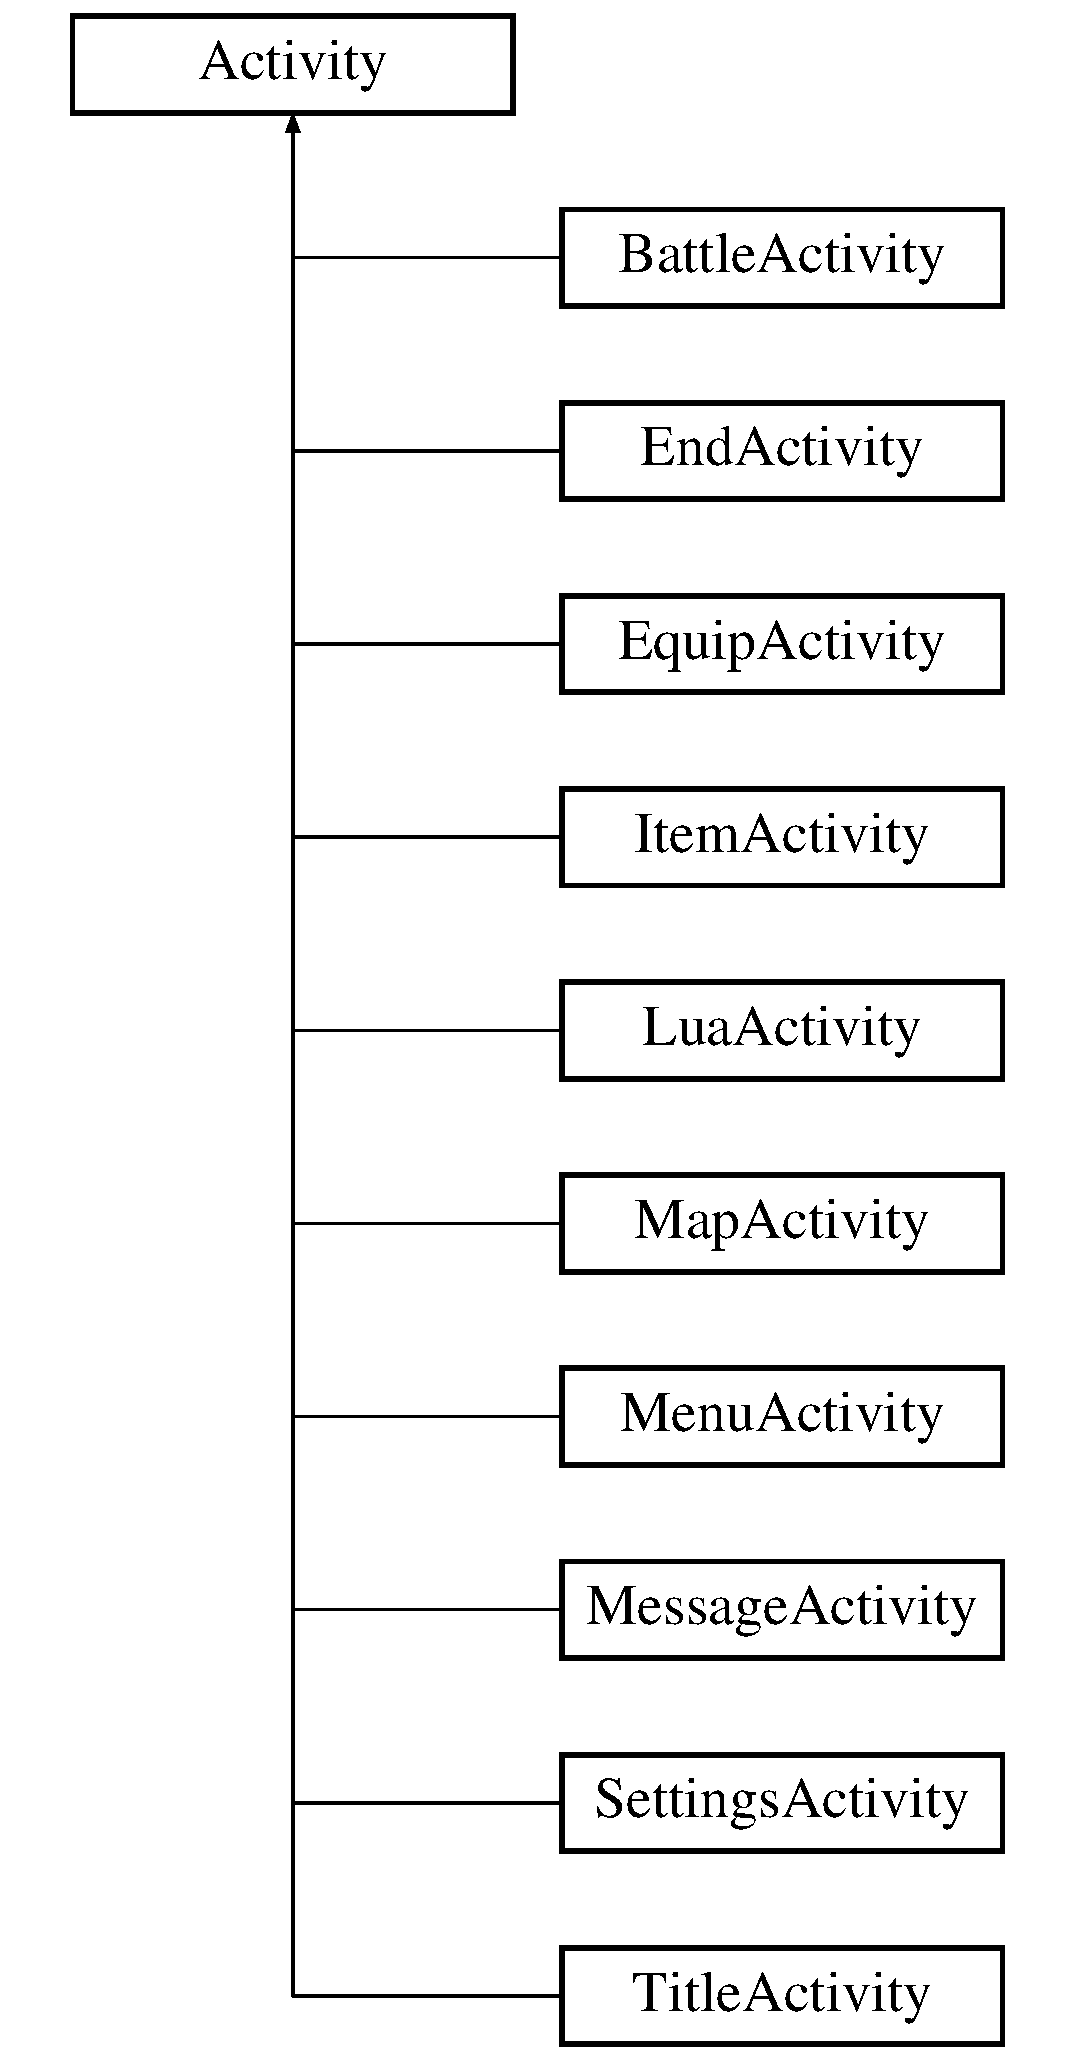
\includegraphics[height=11.000000cm]{classActivity}
\end{center}
\end{figure}
\subsection*{Public Types}
\begin{DoxyCompactItemize}
\item 
enum {\bfseries Type} \{ \\*
{\bfseries None}, 
{\bfseries Map}, 
{\bfseries Message}, 
{\bfseries Menu}, 
\\*
{\bfseries Lua}, 
{\bfseries Title\-Screen}, 
{\bfseries Game\-End}, 
{\bfseries Items}, 
\\*
{\bfseries Equip}, 
{\bfseries Battle\-Act}
 \}
\end{DoxyCompactItemize}
\subsection*{Public Member Functions}
\begin{DoxyCompactItemize}
\item 
\hypertarget{classActivity_aa5ac7df38f7513ef37986a6252ac0a76}{{\bfseries Activity} (\hyperlink{classActivity}{Activity} $\ast$parent=N\-U\-L\-L)}\label{classActivity_aa5ac7df38f7513ef37986a6252ac0a76}

\item 
\hypertarget{classActivity_aac7476522336d91c0bf5cd4f547d5af7}{virtual void {\bfseries update} ()=0}\label{classActivity_aac7476522336d91c0bf5cd4f547d5af7}

\item 
\hypertarget{classActivity_a8f67a0273dba93784a56822de5aea3c4}{virtual void {\bfseries render} ()=0}\label{classActivity_a8f67a0273dba93784a56822de5aea3c4}

\item 
\hypertarget{classActivity_ab53334424e9f945a3fbcf4570626f847}{void {\bfseries poll\-Events} ()}\label{classActivity_ab53334424e9f945a3fbcf4570626f847}

\item 
\hypertarget{classActivity_a41158dea1149bf543e56a7690101369a}{void {\bfseries render\-Background} ()}\label{classActivity_a41158dea1149bf543e56a7690101369a}

\item 
\hypertarget{classActivity_a018ba1c18ef53dc9c090dae4f2b061af}{void {\bfseries screenshot} (\hyperlink{classActivity}{Activity} $\ast$activity)}\label{classActivity_a018ba1c18ef53dc9c090dae4f2b061af}

\item 
\hypertarget{classActivity_ab2157a3189dc2f765121e2578c6b2c16}{Type {\bfseries type} () const }\label{classActivity_ab2157a3189dc2f765121e2578c6b2c16}

\item 
\hypertarget{classActivity_a60e8fc6db09e906e9dc352c2de0bcccb}{\hyperlink{classActivity}{Activity} $\ast$ {\bfseries parent} () const }\label{classActivity_a60e8fc6db09e906e9dc352c2de0bcccb}

\end{DoxyCompactItemize}
\subsection*{Protected Attributes}
\begin{DoxyCompactItemize}
\item 
\hypertarget{classActivity_a97a995e281ea0edca895d8d0a2e38402}{Type {\bfseries m\-\_\-type}}\label{classActivity_a97a995e281ea0edca895d8d0a2e38402}

\item 
\hypertarget{classActivity_a1296633231a9db265ee50c38ff775eaf}{\hyperlink{classActivity}{Activity} $\ast$ {\bfseries m\-\_\-parent}}\label{classActivity_a1296633231a9db265ee50c38ff775eaf}

\item 
\hypertarget{classActivity_a0583a6d6a451ff54d95a2c058eca992f}{S\-D\-L\-\_\-\-Texture $\ast$ {\bfseries m\-\_\-background}}\label{classActivity_a0583a6d6a451ff54d95a2c058eca992f}

\end{DoxyCompactItemize}


The documentation for this class was generated from the following files\-:\begin{DoxyCompactItemize}
\item 
/home/quentin/\-Projects/\-Asylia/include/activities/Activity.\-hpp\item 
/home/quentin/\-Projects/\-Asylia/source/activities/Activity.\-cpp\end{DoxyCompactItemize}

\hypertarget{classActivityManager}{\section{Activity\-Manager Class Reference}
\label{classActivityManager}\index{Activity\-Manager@{Activity\-Manager}}
}
\subsection*{Static Public Member Functions}
\begin{DoxyCompactItemize}
\item 
\hypertarget{classActivityManager_a59f65b6fc5772088b35d9d4d062db793}{static void {\bfseries init} ()}\label{classActivityManager_a59f65b6fc5772088b35d9d4d062db793}

\item 
\hypertarget{classActivityManager_ab7470be868beeb92ffba805bd53441fb}{static void {\bfseries free} ()}\label{classActivityManager_ab7470be868beeb92ffba805bd53441fb}

\item 
\hypertarget{classActivityManager_af4e91287c2f04b5c3fc8619c108998b8}{static \hyperlink{classActivity}{Activity} $\ast$ {\bfseries top} ()}\label{classActivityManager_af4e91287c2f04b5c3fc8619c108998b8}

\item 
\hypertarget{classActivityManager_a7bb249958444325228d66431c1d03978}{static void {\bfseries pop} ()}\label{classActivityManager_a7bb249958444325228d66431c1d03978}

\item 
\hypertarget{classActivityManager_aeb64df781f0e5322abf768ec60e6f0fc}{static void {\bfseries push} (\hyperlink{classActivity}{Activity} $\ast$activity)}\label{classActivityManager_aeb64df781f0e5322abf768ec60e6f0fc}

\item 
\hypertarget{classActivityManager_ab0d3a3ee6d0164a4b474c6ee2094fa7f}{static int {\bfseries size} ()}\label{classActivityManager_ab0d3a3ee6d0164a4b474c6ee2094fa7f}

\item 
\hypertarget{classActivityManager_a514ebca0ffbfdae234fa887fadf91d02}{static \hyperlink{classMessageActivity}{Message\-Activity} $\ast$ {\bfseries draw\-Message} (std\-::string message)}\label{classActivityManager_a514ebca0ffbfdae234fa887fadf91d02}

\item 
\hypertarget{classActivityManager_a855105c4230af046eab6e6e8bcf08ba5}{static \hyperlink{classBattleActivity}{Battle\-Activity} $\ast$ {\bfseries start\-Battle} (u16 id, bool allow\-Defeat)}\label{classActivityManager_a855105c4230af046eab6e6e8bcf08ba5}

\end{DoxyCompactItemize}
\subsection*{Static Public Attributes}
\begin{DoxyCompactItemize}
\item 
\hypertarget{classActivityManager_a752d2002bd19e545da154537977aa7d6}{static std\-::stack$<$ \hyperlink{classActivity}{Activity} $\ast$ $>$ {\bfseries activities}}\label{classActivityManager_a752d2002bd19e545da154537977aa7d6}

\end{DoxyCompactItemize}


The documentation for this class was generated from the following files\-:\begin{DoxyCompactItemize}
\item 
/home/quentin/\-Projects/\-Asylia/include/managers/Activity\-Manager.\-hpp\item 
/home/quentin/\-Projects/\-Asylia/source/managers/Activity\-Manager.\-cpp\end{DoxyCompactItemize}

\hypertarget{classActor}{\section{Actor Class Reference}
\label{classActor}\index{Actor@{Actor}}
}
Inheritance diagram for Actor\-:\begin{figure}[H]
\begin{center}
\leavevmode
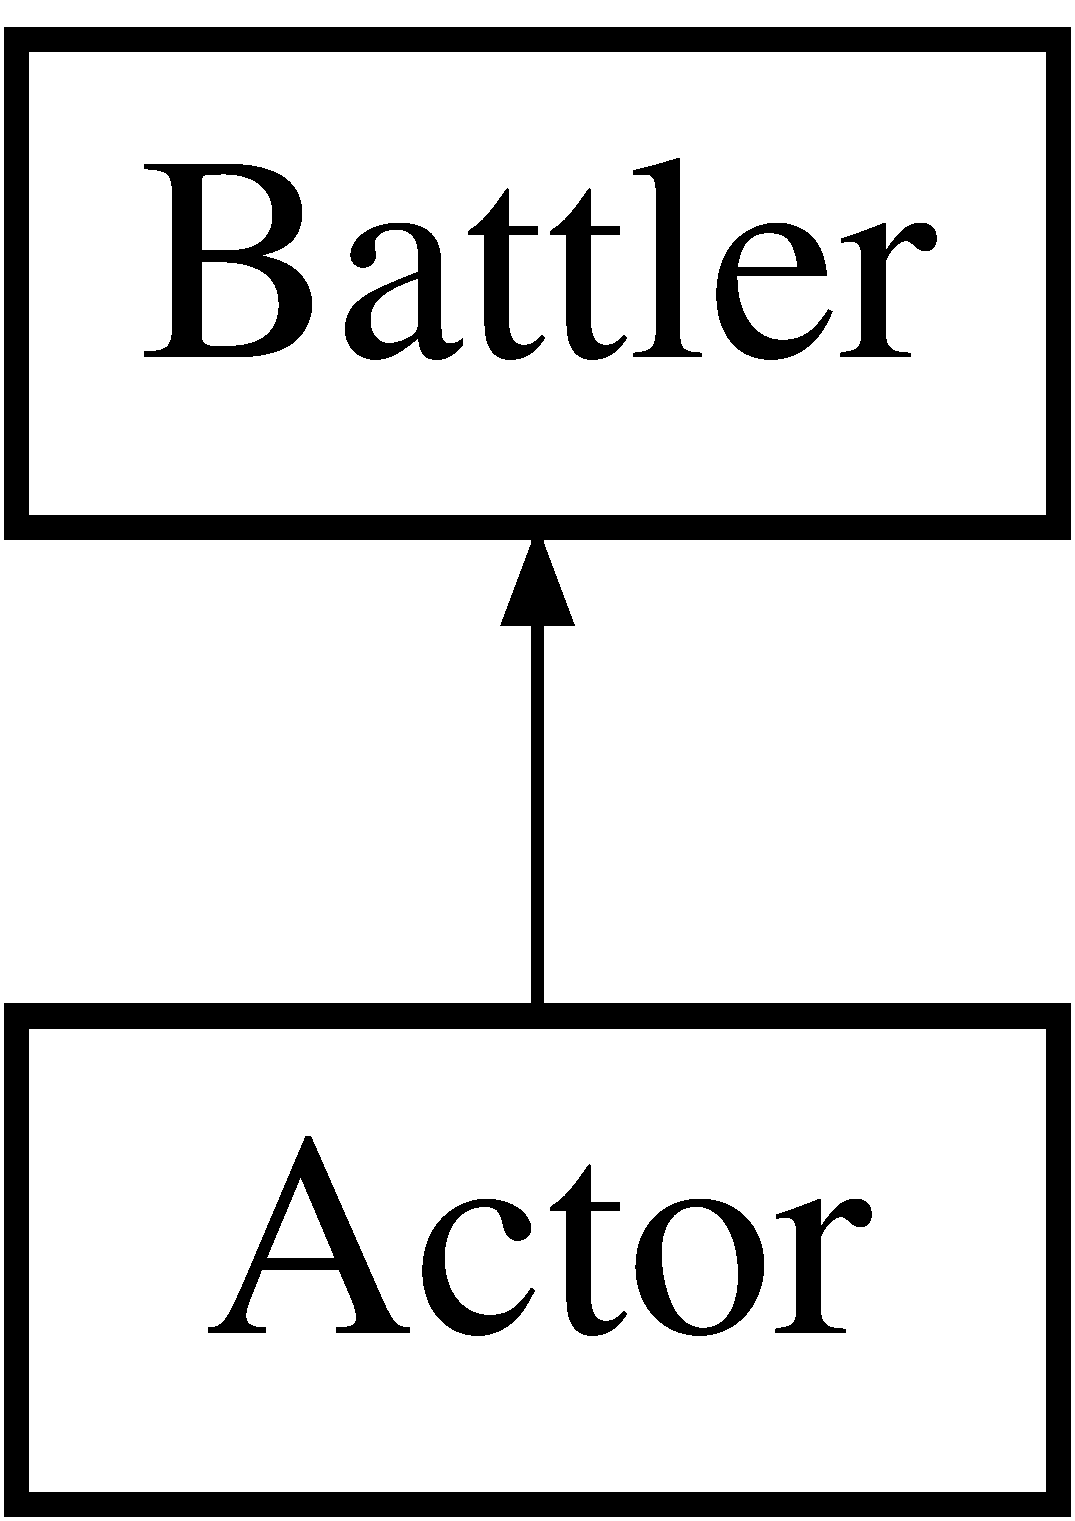
\includegraphics[height=2.000000cm]{classActor}
\end{center}
\end{figure}
\subsection*{Public Member Functions}
\begin{DoxyCompactItemize}
\item 
\hypertarget{classActor_ad798fd68e9d080201facb0e497fac994}{{\bfseries Actor} (std\-::string name, std\-::string appearance, u8 level)}\label{classActor_ad798fd68e9d080201facb0e497fac994}

\item 
\hypertarget{classActor_a284d982f35bc080b5893a1a13d54ca32}{u16 {\bfseries total\-Atk} ()}\label{classActor_a284d982f35bc080b5893a1a13d54ca32}

\item 
\hypertarget{classActor_af59a0165a200c79d463ffe25eb8e6623}{u16 {\bfseries total\-Def} ()}\label{classActor_af59a0165a200c79d463ffe25eb8e6623}

\item 
\hypertarget{classActor_a9d2f1351d7cb086cf5dc62deca40c76b}{\hyperlink{classEquipment}{Equipment} $\ast$ {\bfseries equipment} ()}\label{classActor_a9d2f1351d7cb086cf5dc62deca40c76b}

\end{DoxyCompactItemize}
\subsection*{Additional Inherited Members}


The documentation for this class was generated from the following files\-:\begin{DoxyCompactItemize}
\item 
/home/quentin/\-Projects/\-Asylia/include/entities/Actor.\-hpp\item 
/home/quentin/\-Projects/\-Asylia/source/entities/Actor.\-cpp\end{DoxyCompactItemize}

\hypertarget{classActorChoiceWindow}{\section{Actor\-Choice\-Window Class Reference}
\label{classActorChoiceWindow}\index{Actor\-Choice\-Window@{Actor\-Choice\-Window}}
}
Inheritance diagram for Actor\-Choice\-Window\-:\begin{figure}[H]
\begin{center}
\leavevmode
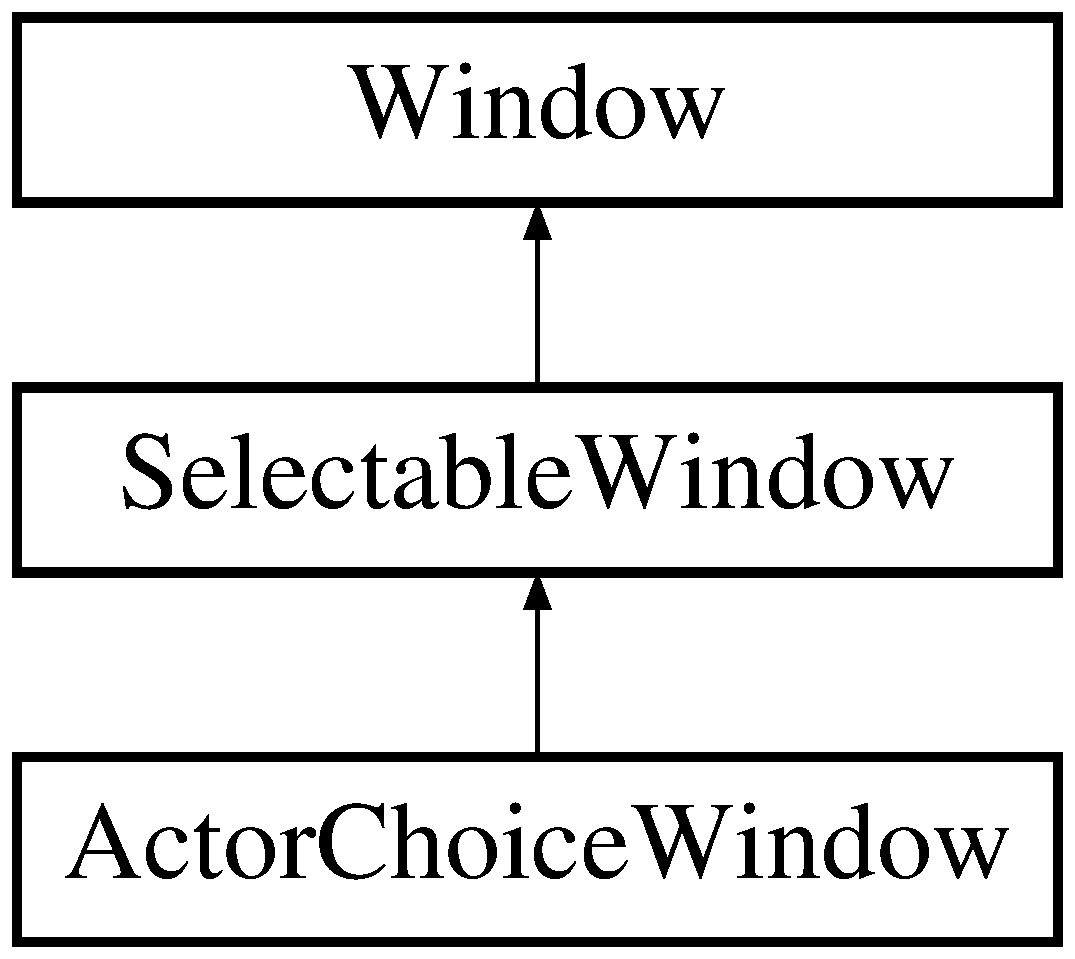
\includegraphics[height=3.000000cm]{classActorChoiceWindow}
\end{center}
\end{figure}
\subsection*{Public Member Functions}
\begin{DoxyCompactItemize}
\item 
\hypertarget{classActorChoiceWindow_a49873e3cb59f9f7970b8ed598a5a7dd9}{{\bfseries Actor\-Choice\-Window} (s16 x, s16 y, u16 width, u16 height)}\label{classActorChoiceWindow_a49873e3cb59f9f7970b8ed598a5a7dd9}

\item 
\hypertarget{classActorChoiceWindow_a2e78b977b6d1162de3b7810d91c178e3}{void {\bfseries update} ()}\label{classActorChoiceWindow_a2e78b977b6d1162de3b7810d91c178e3}

\item 
\hypertarget{classActorChoiceWindow_af4a4e8b9c02fbd986de9117c633d1f81}{void {\bfseries draw\-Actor} (u16 pos)}\label{classActorChoiceWindow_af4a4e8b9c02fbd986de9117c633d1f81}

\item 
\hypertarget{classActorChoiceWindow_a4517b46c73ba16ab8ed00ca57a71b11e}{void {\bfseries draw} ()}\label{classActorChoiceWindow_a4517b46c73ba16ab8ed00ca57a71b11e}

\end{DoxyCompactItemize}
\subsection*{Additional Inherited Members}


The documentation for this class was generated from the following files\-:\begin{DoxyCompactItemize}
\item 
/home/quentin/\-Projects/\-Asylia/include/windows/Actor\-Choice\-Window.\-hpp\item 
/home/quentin/\-Projects/\-Asylia/source/windows/Actor\-Choice\-Window.\-cpp\end{DoxyCompactItemize}

\hypertarget{classActorStatsWindow}{\section{Actor\-Stats\-Window Class Reference}
\label{classActorStatsWindow}\index{Actor\-Stats\-Window@{Actor\-Stats\-Window}}
}
Inheritance diagram for Actor\-Stats\-Window\-:\begin{figure}[H]
\begin{center}
\leavevmode
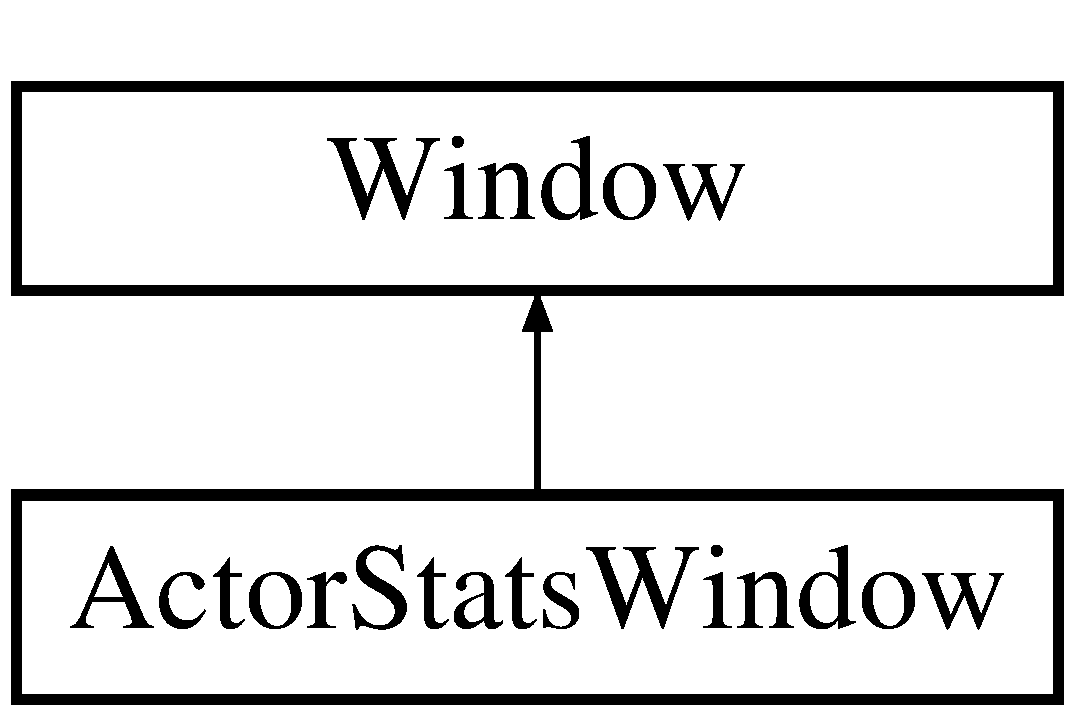
\includegraphics[height=2.000000cm]{classActorStatsWindow}
\end{center}
\end{figure}
\subsection*{Public Member Functions}
\begin{DoxyCompactItemize}
\item 
\hypertarget{classActorStatsWindow_a6d3183b98676321266e9dcf521539da8}{void {\bfseries draw\-Actors} (std\-::vector$<$ std\-::pair$<$ u8, \hyperlink{classActor}{Actor} $\ast$ $>$$>$ actors)}\label{classActorStatsWindow_a6d3183b98676321266e9dcf521539da8}

\item 
\hypertarget{classActorStatsWindow_a23bbdc3900d258e383dbc587ee54c9b3}{void {\bfseries draw\-Actor} (\hyperlink{classActor}{Actor} $\ast$actor, u8 pos)}\label{classActorStatsWindow_a23bbdc3900d258e383dbc587ee54c9b3}

\item 
\hypertarget{classActorStatsWindow_a3d4107851aca473952c649174debe167}{void {\bfseries draw\-Enemies} (std\-::vector$<$ std\-::pair$<$ u8, \hyperlink{classEnemy}{Enemy} $\ast$ $>$$>$ enemies)}\label{classActorStatsWindow_a3d4107851aca473952c649174debe167}

\item 
\hypertarget{classActorStatsWindow_aa1b7fbbc383eacf191fe3dbca2407f3d}{void {\bfseries draw\-Enemy} (\hyperlink{classEnemy}{Enemy} $\ast$enemy, u8 pos, u8 max)}\label{classActorStatsWindow_aa1b7fbbc383eacf191fe3dbca2407f3d}

\end{DoxyCompactItemize}
\subsection*{Additional Inherited Members}


The documentation for this class was generated from the following files\-:\begin{DoxyCompactItemize}
\item 
/home/quentin/\-Projects/\-Asylia/include/windows/Actor\-Stats\-Window.\-hpp\item 
/home/quentin/\-Projects/\-Asylia/source/windows/Actor\-Stats\-Window.\-cpp\end{DoxyCompactItemize}

\hypertarget{classAnimation}{\section{Animation Class Reference}
\label{classAnimation}\index{Animation@{Animation}}
}
Inheritance diagram for Animation\-:\begin{figure}[H]
\begin{center}
\leavevmode
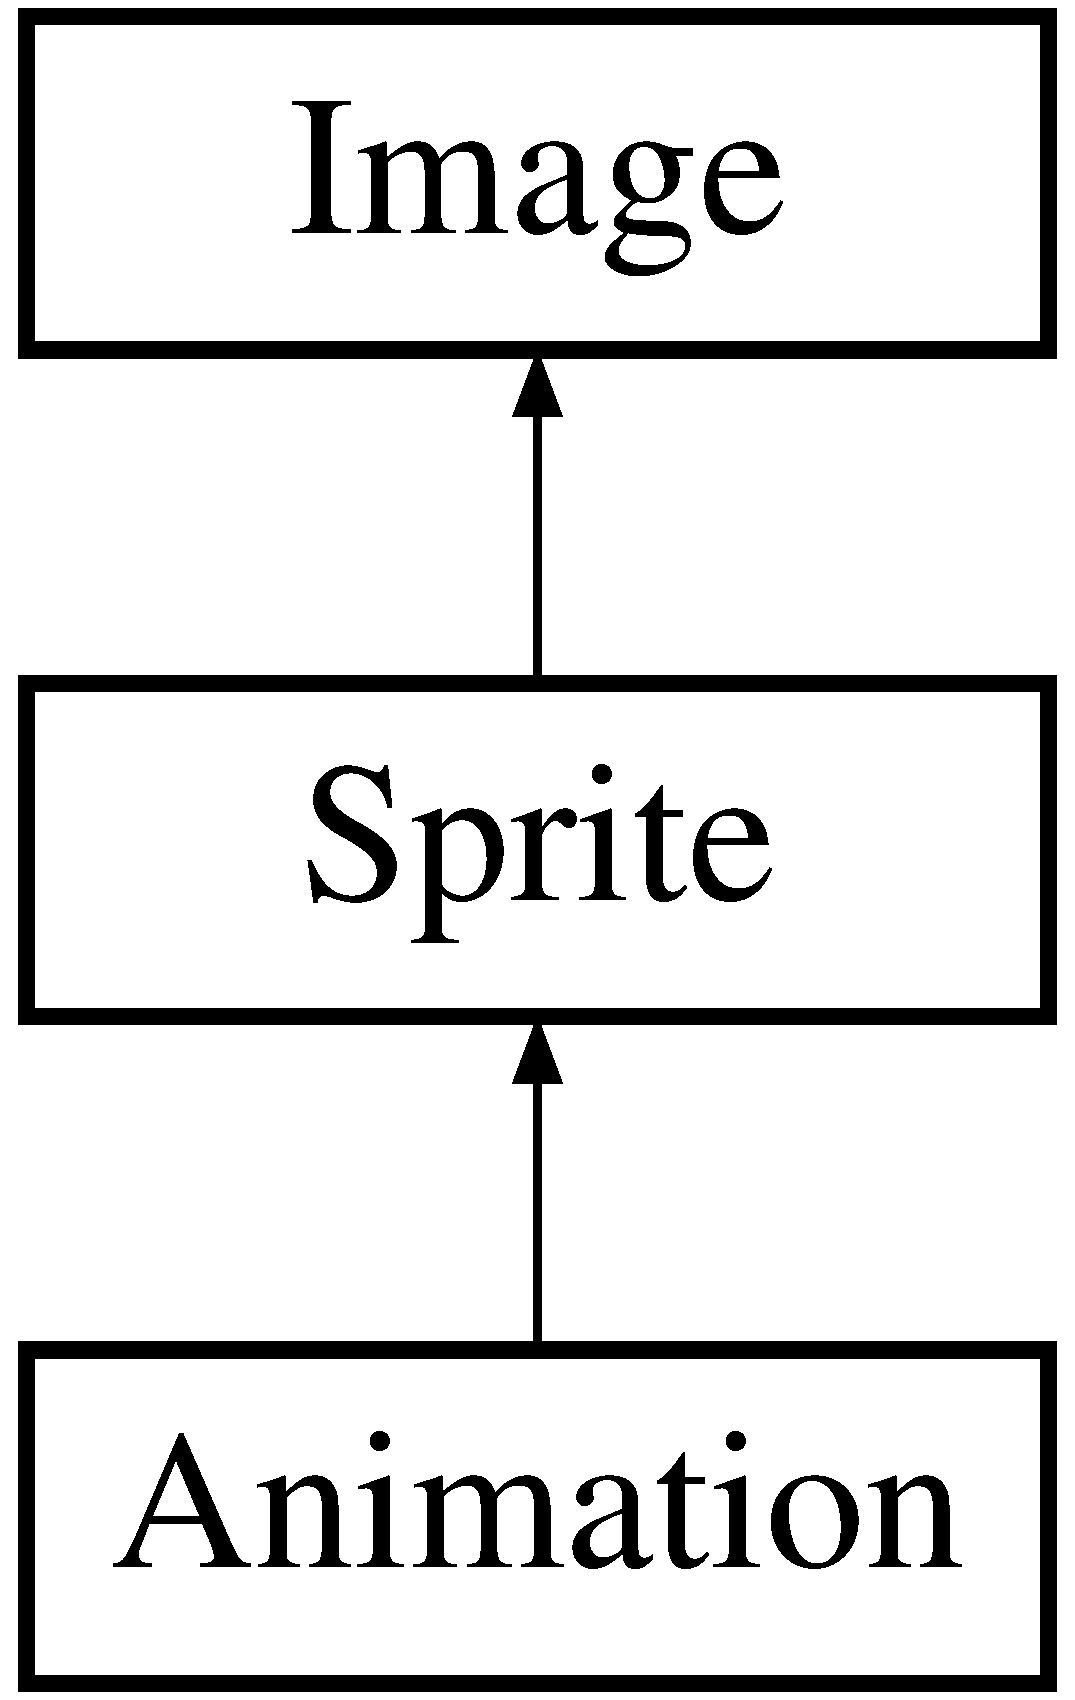
\includegraphics[height=3.000000cm]{classAnimation}
\end{center}
\end{figure}
\subsection*{Public Member Functions}
\begin{DoxyCompactItemize}
\item 
\hypertarget{classAnimation_a0dd517adfab513455eadab94fad105bb}{{\bfseries Animation} (const char $\ast$filename, std\-::string name, u16 delay, std\-::vector$<$ u16 $>$ frames, u16 frame\-Width=192, u16 frame\-Height=192)}\label{classAnimation_a0dd517adfab513455eadab94fad105bb}

\item 
\hypertarget{classAnimation_a5dd394af4c0a5ee6ae84ff80ae15d3af}{void {\bfseries play} (\hyperlink{classBattler}{Battler} $\ast$target)}\label{classAnimation_a5dd394af4c0a5ee6ae84ff80ae15d3af}

\item 
\hypertarget{classAnimation_aa04c1b77a06e3e161063fb5c48a76042}{std\-::string {\bfseries name} () const }\label{classAnimation_aa04c1b77a06e3e161063fb5c48a76042}

\end{DoxyCompactItemize}
\subsection*{Additional Inherited Members}


The documentation for this class was generated from the following files\-:\begin{DoxyCompactItemize}
\item 
/home/quentin/\-Projects/\-Asylia/include/display/Animation.\-hpp\item 
/home/quentin/\-Projects/\-Asylia/source/display/Animation.\-cpp\end{DoxyCompactItemize}

\hypertarget{classArmor}{\section{Armor Class Reference}
\label{classArmor}\index{Armor@{Armor}}
}
Inheritance diagram for Armor\-:\begin{figure}[H]
\begin{center}
\leavevmode
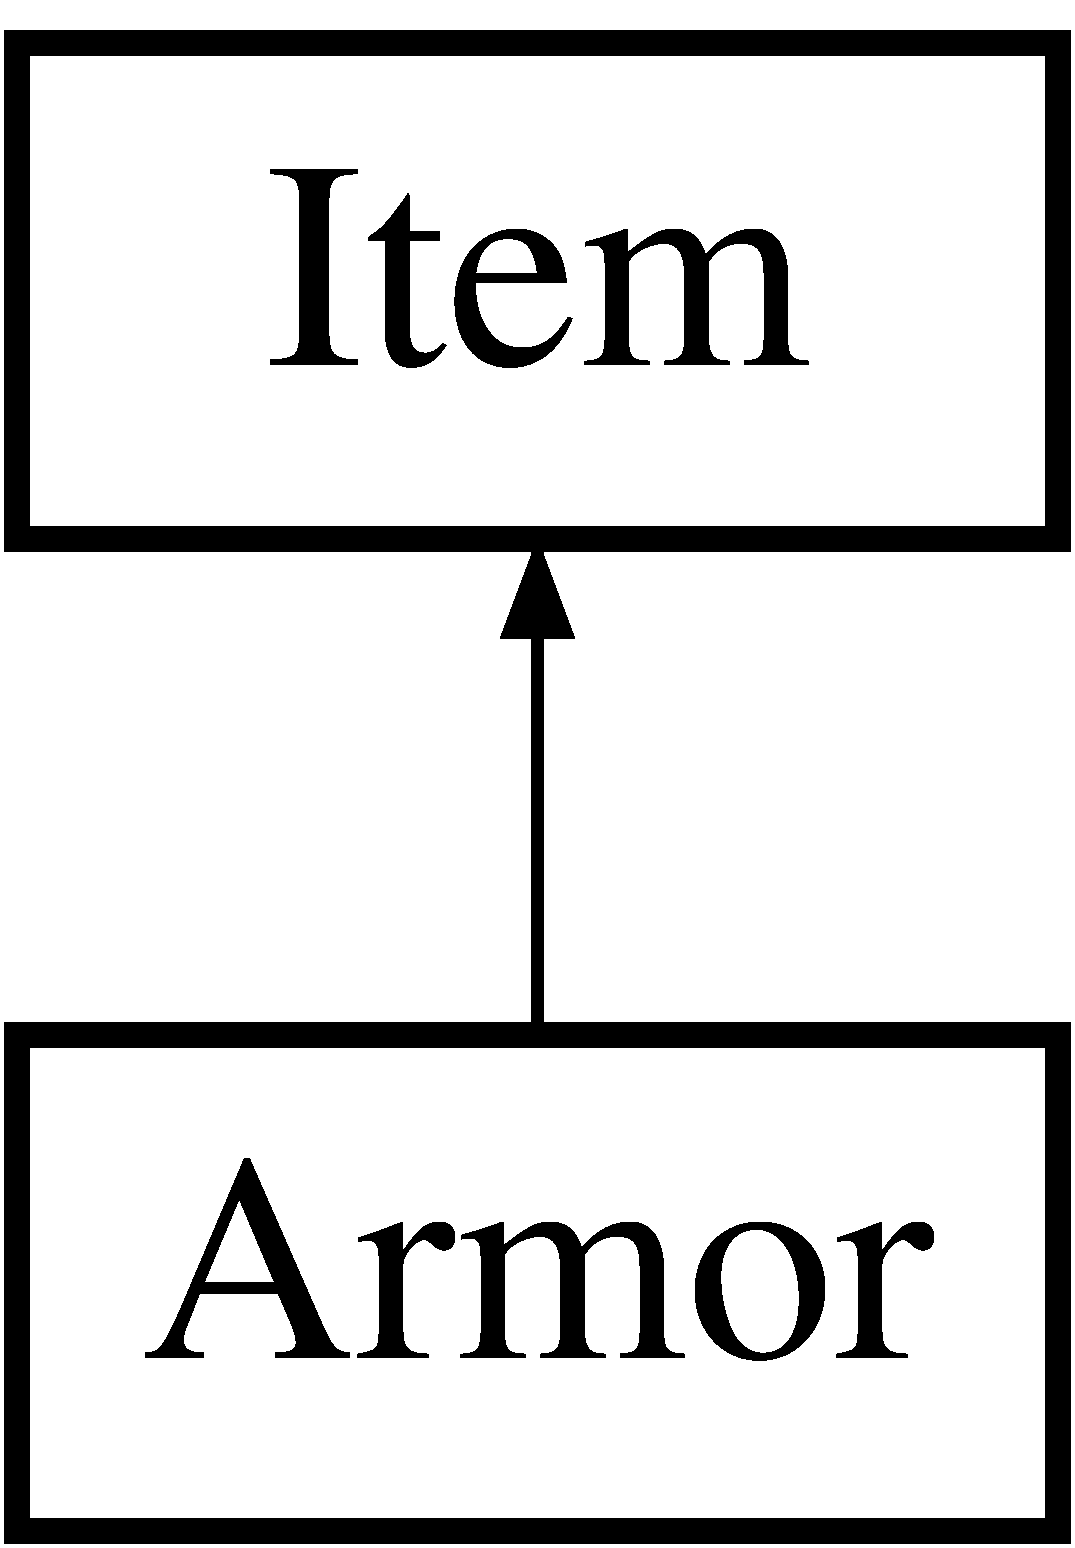
\includegraphics[height=2.000000cm]{classArmor}
\end{center}
\end{figure}
\subsection*{Public Member Functions}
\begin{DoxyCompactItemize}
\item 
\hypertarget{classArmor_a8c42e1c1a19f27b5728bf36f8c509d5a}{{\bfseries Armor} (std\-::string name, std\-::string description, std\-::string thumbnail, u8 slot, u16 def)}\label{classArmor_a8c42e1c1a19f27b5728bf36f8c509d5a}

\item 
\hypertarget{classArmor_a7e46068e1b88c09db3dedcbe1bf9a07d}{u8 {\bfseries slot} () const }\label{classArmor_a7e46068e1b88c09db3dedcbe1bf9a07d}

\item 
\hypertarget{classArmor_a2eff0e2ed2de67be709af24e0f609a49}{u16 {\bfseries def} () const }\label{classArmor_a2eff0e2ed2de67be709af24e0f609a49}

\end{DoxyCompactItemize}
\subsection*{Additional Inherited Members}


The documentation for this class was generated from the following files\-:\begin{DoxyCompactItemize}
\item 
/home/quentin/\-Projects/\-Asylia/include/objects/Armor.\-hpp\item 
/home/quentin/\-Projects/\-Asylia/source/objects/Armor.\-cpp\end{DoxyCompactItemize}

\hypertarget{classBattle}{\section{Battle Class Reference}
\label{classBattle}\index{Battle@{Battle}}
}
\subsection*{Public Member Functions}
\begin{DoxyCompactItemize}
\item 
\hypertarget{classBattle_a81daf6510851cfa958fe31eed732df8d}{{\bfseries Battle} (const \hyperlink{classBattle}{Battle} \&battle)}\label{classBattle_a81daf6510851cfa958fe31eed732df8d}

\item 
\hypertarget{classBattle_a04a4559e884edb5e10d78f4fc002a214}{void {\bfseries add\-Actor} (\hyperlink{classActor}{Actor} $\ast$actor)}\label{classBattle_a04a4559e884edb5e10d78f4fc002a214}

\item 
\hypertarget{classBattle_adb81ba8d0686cf26f7f8e367b9f62501}{void {\bfseries add\-Troop} (\hyperlink{classTroop}{Troop} $\ast$troop)}\label{classBattle_adb81ba8d0686cf26f7f8e367b9f62501}

\item 
\hypertarget{classBattle_a8475a0892e63c2c5882e64a33f92e2ad}{void {\bfseries add\-Enemy} (\hyperlink{classEnemy}{Enemy} $\ast$enemy, s16 x, s16 y)}\label{classBattle_a8475a0892e63c2c5882e64a33f92e2ad}

\item 
\hypertarget{classBattle_a8d3bbc992eb15e85a3b7de2b4cc34cf7}{void {\bfseries draw\-Arrow} (\hyperlink{classBattler}{Battler} $\ast$battler)}\label{classBattle_a8d3bbc992eb15e85a3b7de2b4cc34cf7}

\item 
\hypertarget{classBattle_ac1a5e1a8c51f1de78f371c764f5b4f47}{void {\bfseries enemy\-Turn} ()}\label{classBattle_ac1a5e1a8c51f1de78f371c764f5b4f47}

\item 
\hypertarget{classBattle_a9630440de6cf1087bc8e3fa3f723996c}{void {\bfseries push\-Action} (\hyperlink{classBattler}{Battler} $\ast$actor, \hyperlink{classBattler}{Battler} $\ast$receiver, \hyperlink{classItem}{Item} $\ast$item)}\label{classBattle_a9630440de6cf1087bc8e3fa3f723996c}

\item 
\hypertarget{classBattle_a24d3d1baf830e9bece9618176b426dd2}{void {\bfseries process\-Action} ()}\label{classBattle_a24d3d1baf830e9bece9618176b426dd2}

\item 
\hypertarget{classBattle_a5ee8750acd3f8f3b1cf0c4423cb67eb5}{void {\bfseries update\-Action} ()}\label{classBattle_a5ee8750acd3f8f3b1cf0c4423cb67eb5}

\item 
\hypertarget{classBattle_a0ed5e501d9a58266cd17b6d611a494fb}{bool {\bfseries draw\-Action} ()}\label{classBattle_a0ed5e501d9a58266cd17b6d611a494fb}

\item 
\hypertarget{classBattle_a3e0bd6a620253948e430ec53b4f04672}{void {\bfseries pop\-Action} ()}\label{classBattle_a3e0bd6a620253948e430ec53b4f04672}

\item 
\hypertarget{classBattle_ad35eb3ff6846f7965abf6fe0b3db2f96}{bool {\bfseries action\-Stack\-Empty} ()}\label{classBattle_ad35eb3ff6846f7965abf6fe0b3db2f96}

\item 
\hypertarget{classBattle_a186a9ef5c51b9dbc2acc88e1ad032e02}{void {\bfseries check\-Dead} ()}\label{classBattle_a186a9ef5c51b9dbc2acc88e1ad032e02}

\item 
\hypertarget{classBattle_a45aa1b27b7a4151ed7101ac9a1e347d5}{void {\bfseries sort\-Battle\-Actions} ()}\label{classBattle_a45aa1b27b7a4151ed7101ac9a1e347d5}

\item 
\hypertarget{classBattle_a95cc7e1f4228d2adba39aa1664651c1f}{\hyperlink{classActor}{Actor} $\ast$ {\bfseries get\-Actor} (u8 id)}\label{classBattle_a95cc7e1f4228d2adba39aa1664651c1f}

\item 
\hypertarget{classBattle_ac7e10fe83e378adf7c3cdcfd2ea43287}{\hyperlink{classEnemy}{Enemy} $\ast$ {\bfseries get\-Enemy} (u8 id)}\label{classBattle_ac7e10fe83e378adf7c3cdcfd2ea43287}

\item 
\hypertarget{classBattle_afb01e330972bc83131fb5906d69bc706}{u8 {\bfseries get\-Actor\-Pos} (u8 id)}\label{classBattle_afb01e330972bc83131fb5906d69bc706}

\item 
\hypertarget{classBattle_a5ff82f19a80e8f97eff3beda6e18b9e7}{u8 {\bfseries get\-Enemy\-Pos} (u8 id)}\label{classBattle_a5ff82f19a80e8f97eff3beda6e18b9e7}

\item 
\hypertarget{classBattle_ae20d56d9d9a4c552e0c889c1734a8340}{std\-::pair$<$ u8, \hyperlink{classActor}{Actor} $\ast$ $>$ {\bfseries get\-Next\-Actor\-Pair} (s8 v, s8 current)}\label{classBattle_ae20d56d9d9a4c552e0c889c1734a8340}

\item 
\hypertarget{classBattle_afc4572d8a6760d86347d798f98f29835}{std\-::pair$<$ u8, \hyperlink{classEnemy}{Enemy} $\ast$ $>$ {\bfseries get\-Next\-Enemy\-Pair} (s8 v, s8 current)}\label{classBattle_afc4572d8a6760d86347d798f98f29835}

\item 
\hypertarget{classBattle_acd364ba3f1f746928d7fba884d3a786a}{std\-::vector$<$ std\-::pair$<$ u8, \\*
\hyperlink{classActor}{Actor} $\ast$ $>$ $>$ {\bfseries actors} ()}\label{classBattle_acd364ba3f1f746928d7fba884d3a786a}

\item 
\hypertarget{classBattle_a8c7186d9e2b051c3e35aa4af6335bd98}{std\-::vector$<$ std\-::pair$<$ u8, \\*
\hyperlink{classEnemy}{Enemy} $\ast$ $>$ $>$ {\bfseries enemies} ()}\label{classBattle_a8c7186d9e2b051c3e35aa4af6335bd98}

\item 
\hypertarget{classBattle_ae1b334af1ccf83fb7cba4b00de66962b}{void {\bfseries set\-Battleback} (\hyperlink{classImage}{Image} $\ast$battleback)}\label{classBattle_ae1b334af1ccf83fb7cba4b00de66962b}

\item 
\hypertarget{classBattle_a6e4983c56bd308a7b220fd65a27df3c3}{void {\bfseries render\-Battleback} ()}\label{classBattle_a6e4983c56bd308a7b220fd65a27df3c3}

\item 
\hypertarget{classBattle_a2d70234e3d13c2eb389afde028f93dc8}{u16 {\bfseries exp} () const }\label{classBattle_a2d70234e3d13c2eb389afde028f93dc8}

\item 
\hypertarget{classBattle_adb2b58224ab058e7335a244d5938c192}{u16 {\bfseries gold} () const }\label{classBattle_adb2b58224ab058e7335a244d5938c192}

\end{DoxyCompactItemize}


The documentation for this class was generated from the following files\-:\begin{DoxyCompactItemize}
\item 
/home/quentin/\-Projects/\-Asylia/include/objects/Battle.\-hpp\item 
/home/quentin/\-Projects/\-Asylia/source/objects/Battle.\-cpp\end{DoxyCompactItemize}

\hypertarget{classBattleAction}{\section{Battle\-Action Class Reference}
\label{classBattleAction}\index{Battle\-Action@{Battle\-Action}}
}
\subsection*{Public Member Functions}
\begin{DoxyCompactItemize}
\item 
\hypertarget{classBattleAction_a9b6b05f746e2d9f04b5498f36df9488a}{{\bfseries Battle\-Action} (\hyperlink{classBattler}{Battler} $\ast$actor, \hyperlink{classBattler}{Battler} $\ast$receiver, \hyperlink{classItem}{Item} $\ast$item)}\label{classBattleAction_a9b6b05f746e2d9f04b5498f36df9488a}

\item 
\hypertarget{classBattleAction_ab56443cf3e4d5562ee46efcb65e470d5}{void {\bfseries process} ()}\label{classBattleAction_ab56443cf3e4d5562ee46efcb65e470d5}

\item 
\hypertarget{classBattleAction_ae465e2ef0dd218368d5e006bda4ee978}{void {\bfseries update\-Damages} ()}\label{classBattleAction_ae465e2ef0dd218368d5e006bda4ee978}

\item 
\hypertarget{classBattleAction_af684977431c24f66fe878fc7d068d5cd}{bool {\bfseries draw\-Damages} ()}\label{classBattleAction_af684977431c24f66fe878fc7d068d5cd}

\item 
\hypertarget{classBattleAction_a8c7336976d1554616fe1bf6d649abae4}{\hyperlink{classBattler}{Battler} $\ast$ {\bfseries actor} () const }\label{classBattleAction_a8c7336976d1554616fe1bf6d649abae4}

\item 
\hypertarget{classBattleAction_aac14c90c15d4c88d2cbd5bb201b22ad8}{\hyperlink{classBattler}{Battler} $\ast$ {\bfseries receiver} () const }\label{classBattleAction_aac14c90c15d4c88d2cbd5bb201b22ad8}

\item 
\hypertarget{classBattleAction_a5030a7484d3a6d00376d9ade6e2835f5}{bool {\bfseries animation\-At\-End} () const }\label{classBattleAction_a5030a7484d3a6d00376d9ade6e2835f5}

\item 
\hypertarget{classBattleAction_aa4ad0fe6855848076449398200b188f0}{void {\bfseries set\-Receiver} (\hyperlink{classBattler}{Battler} $\ast$receiver)}\label{classBattleAction_aa4ad0fe6855848076449398200b188f0}

\end{DoxyCompactItemize}


The documentation for this class was generated from the following files\-:\begin{DoxyCompactItemize}
\item 
/home/quentin/\-Projects/\-Asylia/include/objects/Battle\-Action.\-hpp\item 
/home/quentin/\-Projects/\-Asylia/source/objects/Battle\-Action.\-cpp\end{DoxyCompactItemize}

\hypertarget{classBattleActionWindow}{\section{Battle\-Action\-Window Class Reference}
\label{classBattleActionWindow}\index{Battle\-Action\-Window@{Battle\-Action\-Window}}
}
Inheritance diagram for Battle\-Action\-Window\-:\begin{figure}[H]
\begin{center}
\leavevmode
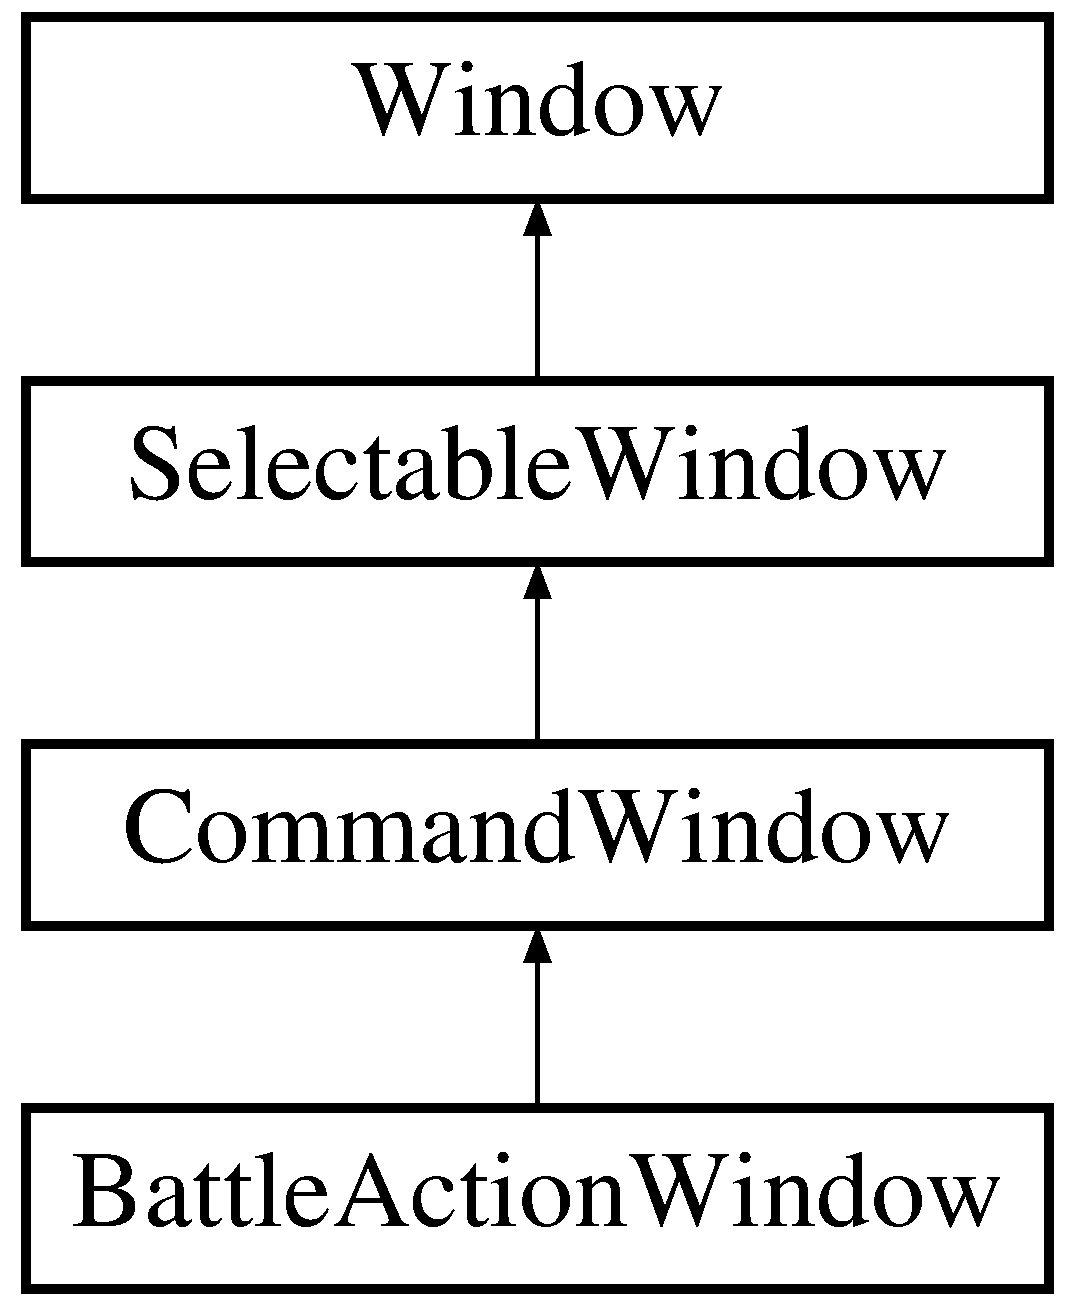
\includegraphics[height=4.000000cm]{classBattleActionWindow}
\end{center}
\end{figure}
\subsection*{Public Member Functions}
\begin{DoxyCompactItemize}
\item 
\hypertarget{classBattleActionWindow_a69934cbf60e25e06ae36690c9fd7babd}{void {\bfseries draw} (u8 pos)}\label{classBattleActionWindow_a69934cbf60e25e06ae36690c9fd7babd}

\end{DoxyCompactItemize}
\subsection*{Additional Inherited Members}


The documentation for this class was generated from the following files\-:\begin{DoxyCompactItemize}
\item 
/home/quentin/\-Projects/\-Asylia/include/windows/Battle\-Action\-Window.\-hpp\item 
/home/quentin/\-Projects/\-Asylia/source/windows/Battle\-Action\-Window.\-cpp\end{DoxyCompactItemize}

\hypertarget{classBattleActivity}{\section{Battle\-Activity Class Reference}
\label{classBattleActivity}\index{Battle\-Activity@{Battle\-Activity}}
}
Inheritance diagram for Battle\-Activity\-:\begin{figure}[H]
\begin{center}
\leavevmode
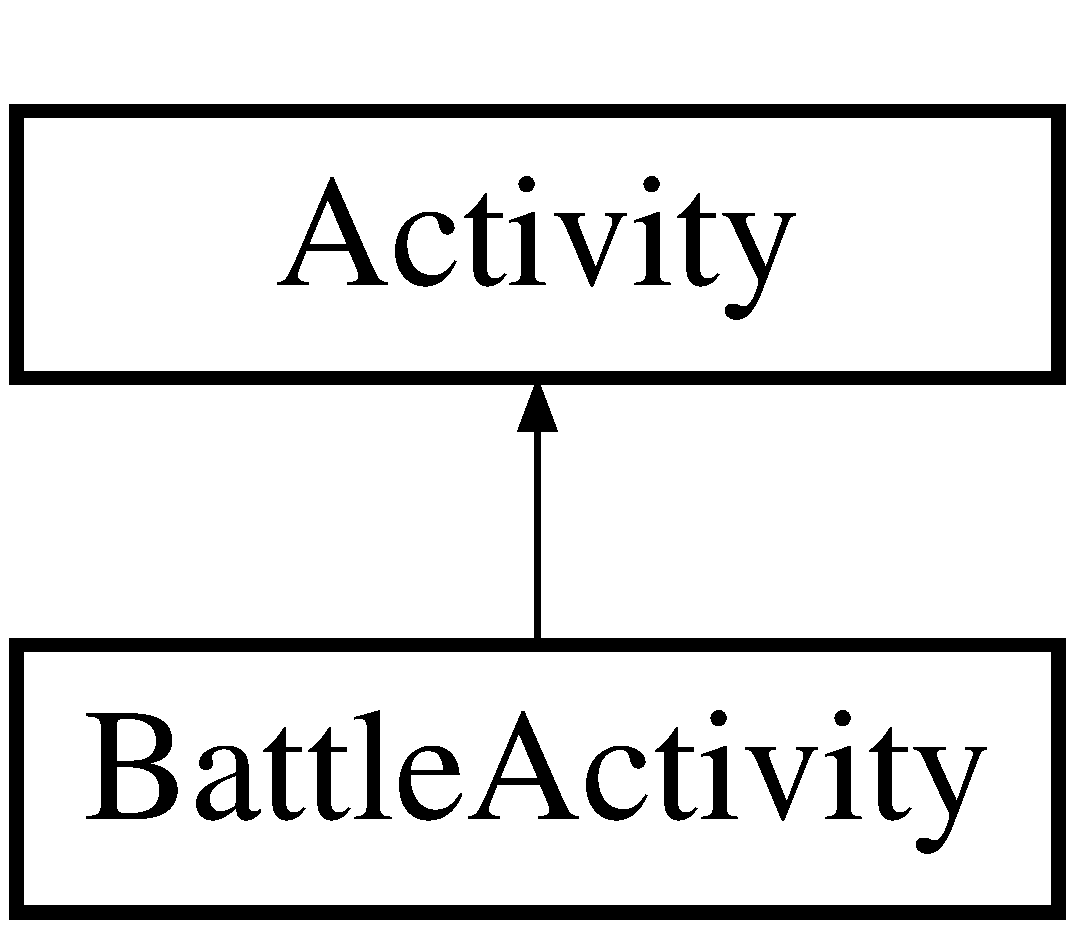
\includegraphics[height=2.000000cm]{classBattleActivity}
\end{center}
\end{figure}
\subsection*{Public Types}
\begin{DoxyCompactItemize}
\item 
enum {\bfseries Mode} \{ \\*
{\bfseries Choice}, 
{\bfseries Action}, 
{\bfseries Item\-Win}, 
{\bfseries Choose\-Actor\-Target}, 
\\*
{\bfseries Choose\-Enemy\-Target}, 
{\bfseries Enemy\-Turn}, 
{\bfseries Process\-Actions}, 
{\bfseries Game\-Over}, 
\\*
{\bfseries Victory}
 \}
\end{DoxyCompactItemize}
\subsection*{Public Member Functions}
\begin{DoxyCompactItemize}
\item 
\hypertarget{classBattleActivity_ab129ed3685823d9c789fc48e0a097b81}{{\bfseries Battle\-Activity} (\hyperlink{classTroop}{Troop} $\ast$troop, bool allow\-Defeat=false)}\label{classBattleActivity_ab129ed3685823d9c789fc48e0a097b81}

\item 
\hypertarget{classBattleActivity_ac04947ecdf5d2fe6da8f0a11c9525379}{void {\bfseries update} ()}\label{classBattleActivity_ac04947ecdf5d2fe6da8f0a11c9525379}

\item 
\hypertarget{classBattleActivity_a64ba166b7d79710c164415454340de8b}{void {\bfseries render} ()}\label{classBattleActivity_a64ba166b7d79710c164415454340de8b}

\item 
\hypertarget{classBattleActivity_adea57ed9fb355bd94b9ec12bc2c3052e}{\hyperlink{classBattle}{Battle} $\ast$ {\bfseries battle} ()}\label{classBattleActivity_adea57ed9fb355bd94b9ec12bc2c3052e}

\item 
\hypertarget{classBattleActivity_a2e82b37fc76a4e7801e0e1b2f28623bb}{s8 {\bfseries current\-Pos} () const }\label{classBattleActivity_a2e82b37fc76a4e7801e0e1b2f28623bb}

\item 
\hypertarget{classBattleActivity_a451a88d0fdb3d4e293e79613bd9cb82e}{u8 {\bfseries mode} () const }\label{classBattleActivity_a451a88d0fdb3d4e293e79613bd9cb82e}

\end{DoxyCompactItemize}
\subsection*{Additional Inherited Members}


The documentation for this class was generated from the following files\-:\begin{DoxyCompactItemize}
\item 
/home/quentin/\-Projects/\-Asylia/include/activities/Battle\-Activity.\-hpp\item 
/home/quentin/\-Projects/\-Asylia/source/activities/Battle\-Activity.\-cpp\end{DoxyCompactItemize}

\hypertarget{classBattleChoiceWindow}{\section{Battle\-Choice\-Window Class Reference}
\label{classBattleChoiceWindow}\index{Battle\-Choice\-Window@{Battle\-Choice\-Window}}
}
Inheritance diagram for Battle\-Choice\-Window\-:\begin{figure}[H]
\begin{center}
\leavevmode
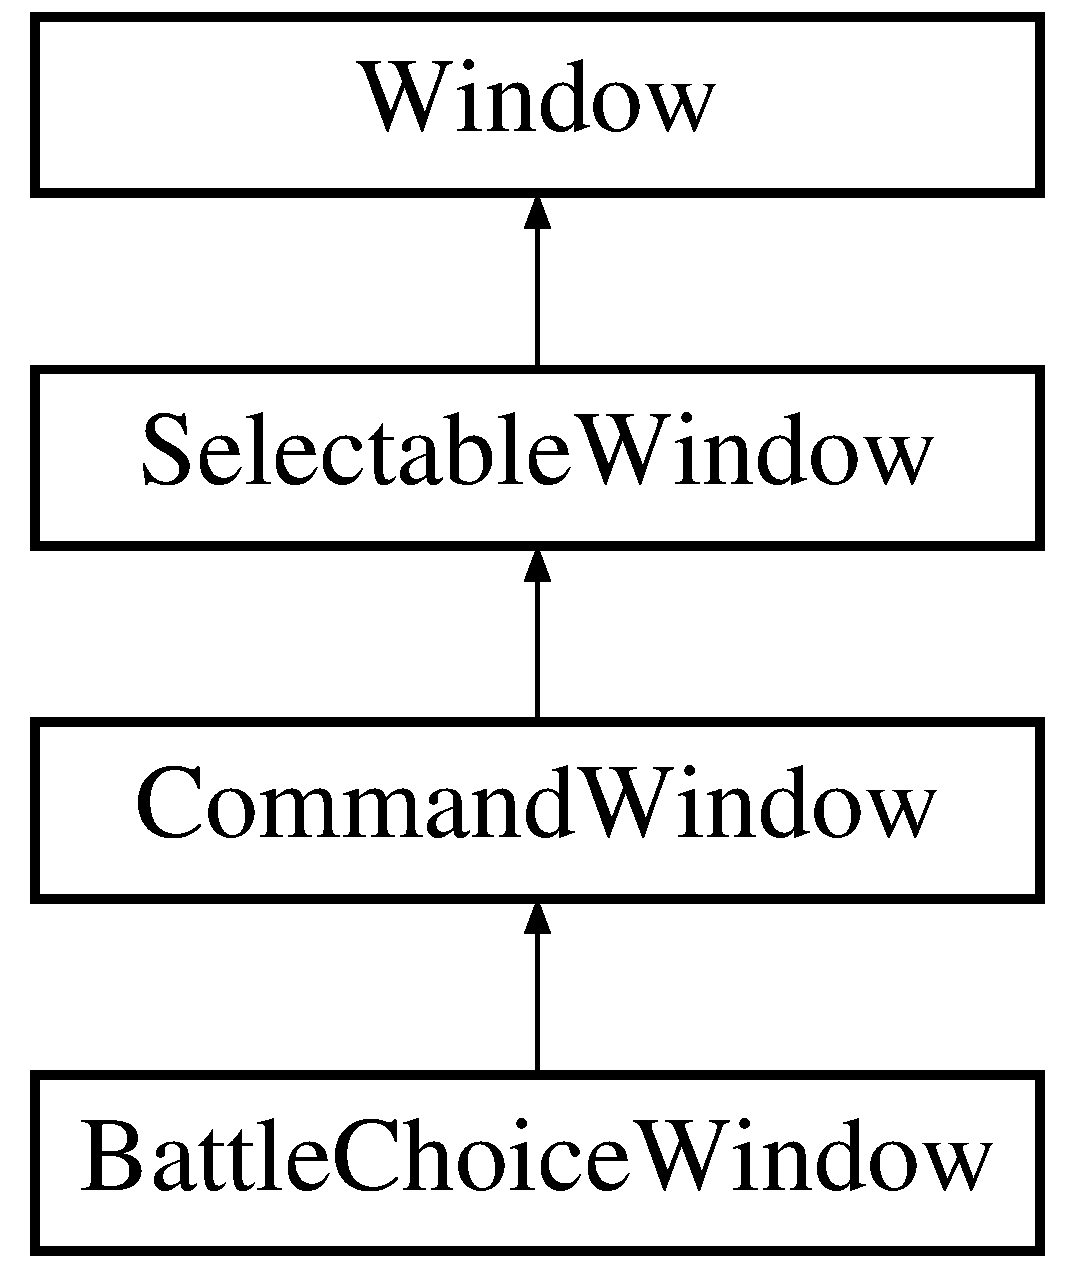
\includegraphics[height=4.000000cm]{classBattleChoiceWindow}
\end{center}
\end{figure}
\subsection*{Additional Inherited Members}


The documentation for this class was generated from the following files\-:\begin{DoxyCompactItemize}
\item 
/home/quentin/\-Projects/\-Asylia/include/windows/Battle\-Choice\-Window.\-hpp\item 
/home/quentin/\-Projects/\-Asylia/source/windows/Battle\-Choice\-Window.\-cpp\end{DoxyCompactItemize}

\hypertarget{classBattler}{\section{Battler Class Reference}
\label{classBattler}\index{Battler@{Battler}}
}
Inheritance diagram for Battler\-:\begin{figure}[H]
\begin{center}
\leavevmode
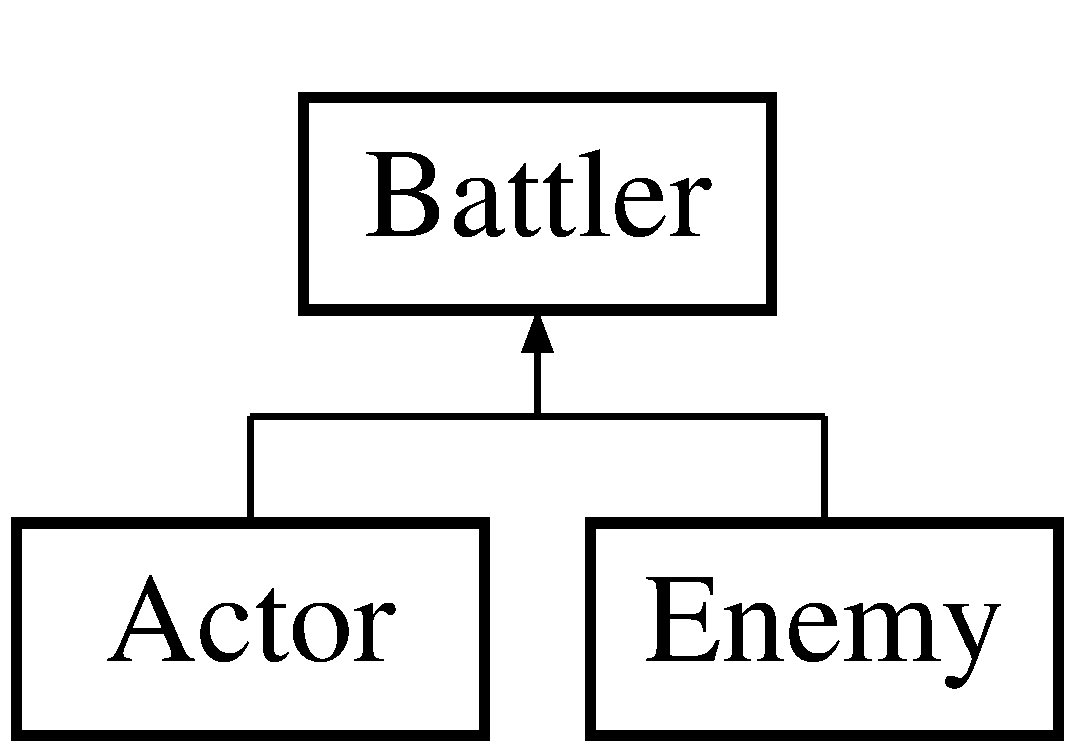
\includegraphics[height=2.000000cm]{classBattler}
\end{center}
\end{figure}
\subsection*{Public Types}
\begin{DoxyCompactItemize}
\item 
enum {\bfseries State} \{ {\bfseries Normal}
 \}
\item 
enum {\bfseries Type} \{ {\bfseries Type\-None}, 
{\bfseries Type\-Actor}, 
{\bfseries Type\-Enemy}
 \}
\end{DoxyCompactItemize}
\subsection*{Public Member Functions}
\begin{DoxyCompactItemize}
\item 
\hypertarget{classBattler_a2dd61dc2fb380da5ce4eb94beae870a4}{{\bfseries Battler} (const \hyperlink{classBattler}{Battler} \&battler)}\label{classBattler_a2dd61dc2fb380da5ce4eb94beae870a4}

\item 
\hypertarget{classBattler_abc682178f335bb6e93a50ae2c0cc14d3}{{\bfseries Battler} (std\-::string name, std\-::string appearance, u8 level)}\label{classBattler_abc682178f335bb6e93a50ae2c0cc14d3}

\item 
\hypertarget{classBattler_aa2135603d74f503b7ea0ba813a3e5751}{void {\bfseries calculate\-All\-Stats} (u16 agi, u16 vit, u16 dex, u16 str, u16 wis, u16 intell)}\label{classBattler_aa2135603d74f503b7ea0ba813a3e5751}

\item 
\hypertarget{classBattler_a1111cc648c06d73b2f51e9f2d036eabc}{void {\bfseries blink} ()}\label{classBattler_a1111cc648c06d73b2f51e9f2d036eabc}

\item 
\hypertarget{classBattler_a13256d68a87e588be4b10438645cffb8}{void {\bfseries kill} ()}\label{classBattler_a13256d68a87e588be4b10438645cffb8}

\item 
\hypertarget{classBattler_a65d0ef219ba0738c750088e7318ad4f8}{std\-::string {\bfseries name} () const }\label{classBattler_a65d0ef219ba0738c750088e7318ad4f8}

\item 
\hypertarget{classBattler_a8c78ffa9f03434f6381fd14bee851c21}{\hyperlink{classImage}{Image} $\ast$ {\bfseries image} () const }\label{classBattler_a8c78ffa9f03434f6381fd14bee851c21}

\item 
\hypertarget{classBattler_a306b9d4a2a15ed27d49266fef3e50e72}{\hyperlink{classSprite}{Sprite} $\ast$ {\bfseries sprite} () const }\label{classBattler_a306b9d4a2a15ed27d49266fef3e50e72}

\item 
\hypertarget{classBattler_aec1f9dc85e5016dffd2e22e277fd4cf4}{u8 {\bfseries level} () const }\label{classBattler_aec1f9dc85e5016dffd2e22e277fd4cf4}

\item 
\hypertarget{classBattler_a8310830b745b7534614582dba4e51e1d}{s16 {\bfseries hp} () const }\label{classBattler_a8310830b745b7534614582dba4e51e1d}

\item 
\hypertarget{classBattler_ab0095f4e3c40c476959e80d7296c0610}{s16 {\bfseries sp} () const }\label{classBattler_ab0095f4e3c40c476959e80d7296c0610}

\item 
\hypertarget{classBattler_a7189a66a907ed930c782425c050eb4d8}{u16 {\bfseries basehp} () const }\label{classBattler_a7189a66a907ed930c782425c050eb4d8}

\item 
\hypertarget{classBattler_aa774f9fbb40dbacdf6b7445931b43767}{u16 {\bfseries basesp} () const }\label{classBattler_aa774f9fbb40dbacdf6b7445931b43767}

\item 
\hypertarget{classBattler_a9784ebe1b564daf8e02d9d68925cb334}{u16 {\bfseries atk} () const }\label{classBattler_a9784ebe1b564daf8e02d9d68925cb334}

\item 
\hypertarget{classBattler_a9dacf59ca3915ecb26049ba227048312}{u16 {\bfseries def} () const }\label{classBattler_a9dacf59ca3915ecb26049ba227048312}

\item 
\hypertarget{classBattler_af6da1484c6da37083b199af9d9aa0b3e}{u16 {\bfseries total\-Atk} () const }\label{classBattler_af6da1484c6da37083b199af9d9aa0b3e}

\item 
\hypertarget{classBattler_aaf91e61dce901c64e7032c6779f5c2ea}{u16 {\bfseries total\-Def} () const }\label{classBattler_aaf91e61dce901c64e7032c6779f5c2ea}

\item 
\hypertarget{classBattler_a656c1b396ab1f97f9ecee83380d5cf21}{u8 {\bfseries state} () const }\label{classBattler_a656c1b396ab1f97f9ecee83380d5cf21}

\item 
\hypertarget{classBattler_a8f3e0edf768a4b22e6e1b63eac4dd594}{u16 {\bfseries exp} () const }\label{classBattler_a8f3e0edf768a4b22e6e1b63eac4dd594}

\item 
\hypertarget{classBattler_af63f631d0f14af0acfa23f5b1a17a375}{void {\bfseries set\-Position} (s16 x, s16 y)}\label{classBattler_af63f631d0f14af0acfa23f5b1a17a375}

\item 
\hypertarget{classBattler_ac6c38c2b25cd94cb6347a1c01f43611c}{void {\bfseries hurt} (u16 damages)}\label{classBattler_ac6c38c2b25cd94cb6347a1c01f43611c}

\item 
\hypertarget{classBattler_ab7a13261d2d559cbbaa0f11d9be80204}{void {\bfseries heal} (u16 p=100)}\label{classBattler_ab7a13261d2d559cbbaa0f11d9be80204}

\item 
\hypertarget{classBattler_a1d6085f40737ed797872a94e338f3601}{std\-::string {\bfseries get\-State\-String} ()}\label{classBattler_a1d6085f40737ed797872a94e338f3601}

\item 
\hypertarget{classBattler_af9922877cc1167a5b79b5245e75adbe7}{void {\bfseries attack} (\hyperlink{classBattler}{Battler} $\ast$battler, \hyperlink{classSkill}{Skill} $\ast$skill)}\label{classBattler_af9922877cc1167a5b79b5245e75adbe7}

\item 
\hypertarget{classBattler_ad653d2ff376d5941db6bc75ba805f5bc}{u8 {\bfseries type} () const }\label{classBattler_ad653d2ff376d5941db6bc75ba805f5bc}

\item 
\hypertarget{classBattler_a3a94f8d955ff7ce42048dc5c12f21905}{u16 {\bfseries grow\-Agi} (u16 agi, u16 level)}\label{classBattler_a3a94f8d955ff7ce42048dc5c12f21905}

\item 
\hypertarget{classBattler_a3aa5681e1b435c136d63854fdeaf256f}{u16 {\bfseries grow\-Vit} (u16 vit, u16 level)}\label{classBattler_a3aa5681e1b435c136d63854fdeaf256f}

\item 
\hypertarget{classBattler_a16c21cc699caa7344c181782a162a97e}{u16 {\bfseries grow\-Dex} (u16 dex, u16 level)}\label{classBattler_a16c21cc699caa7344c181782a162a97e}

\item 
\hypertarget{classBattler_a432a84b99564806a048d704d33751f3a}{u16 {\bfseries grow\-Str} (u16 str, u16 level)}\label{classBattler_a432a84b99564806a048d704d33751f3a}

\item 
\hypertarget{classBattler_a7743cd218d202b911026a7a628793fda}{u16 {\bfseries grow\-Wis} (u16 wis, u16 level)}\label{classBattler_a7743cd218d202b911026a7a628793fda}

\item 
\hypertarget{classBattler_a434a9dbfa8b81860c02aefd180aac7d6}{u16 {\bfseries grow\-Int} (u16 intell, u16 level)}\label{classBattler_a434a9dbfa8b81860c02aefd180aac7d6}

\item 
\hypertarget{classBattler_a6a5bf3e19bbe259eef47d3bb41609f08}{u16 {\bfseries speed} ()}\label{classBattler_a6a5bf3e19bbe259eef47d3bb41609f08}

\item 
\hypertarget{classBattler_ae8624147f877e3b5dd4bf38592699575}{u16 {\bfseries exp\-Given\-If\-Killed} ()}\label{classBattler_ae8624147f877e3b5dd4bf38592699575}

\item 
\hypertarget{classBattler_a2e0be0794cfba7bbc8739e73620dcf0b}{u16 {\bfseries gold\-Given\-If\-Killed} ()}\label{classBattler_a2e0be0794cfba7bbc8739e73620dcf0b}

\item 
\hypertarget{classBattler_a507e4e0eda846d71abee423d22d73520}{s16 {\bfseries exp\-Remaining\-To\-Level\-Up} ()}\label{classBattler_a507e4e0eda846d71abee423d22d73520}

\item 
\hypertarget{classBattler_a38eca67413197a1bdd8c1b405ca64d6f}{void {\bfseries level\-Up} ()}\label{classBattler_a38eca67413197a1bdd8c1b405ca64d6f}

\item 
\hypertarget{classBattler_afef93ce46c3d5ddf15dfeb88777387b3}{void {\bfseries check\-Level\-Up} ()}\label{classBattler_afef93ce46c3d5ddf15dfeb88777387b3}

\item 
\hypertarget{classBattler_a47da85ea8981b9056f7b803642b20485}{void {\bfseries gain\-Exp} (u16 value)}\label{classBattler_a47da85ea8981b9056f7b803642b20485}

\end{DoxyCompactItemize}
\subsection*{Protected Attributes}
\begin{DoxyCompactItemize}
\item 
\hypertarget{classBattler_a9d7fe96eca5e2180869483099bdd0094}{std\-::string {\bfseries m\-\_\-name}}\label{classBattler_a9d7fe96eca5e2180869483099bdd0094}

\item 
\hypertarget{classBattler_adbd67edafe168642e82a6a1fefa31c28}{\hyperlink{classImage}{Image} $\ast$ {\bfseries m\-\_\-image}}\label{classBattler_adbd67edafe168642e82a6a1fefa31c28}

\item 
\hypertarget{classBattler_abbfda09f9cef0aa37c498f0b7b8a7831}{\hyperlink{classSprite}{Sprite} $\ast$ {\bfseries m\-\_\-sprite}}\label{classBattler_abbfda09f9cef0aa37c498f0b7b8a7831}

\item 
\hypertarget{classBattler_a22bd77fbf98347dbefd7f49f2549b433}{u8 {\bfseries m\-\_\-level}}\label{classBattler_a22bd77fbf98347dbefd7f49f2549b433}

\item 
\hypertarget{classBattler_ac47b2c5a307c70e6708c7108e1f5b606}{u16 {\bfseries m\-\_\-exp}}\label{classBattler_ac47b2c5a307c70e6708c7108e1f5b606}

\item 
\hypertarget{classBattler_ad551db1917992557b238d8182300f2c0}{s16 {\bfseries m\-\_\-hp}}\label{classBattler_ad551db1917992557b238d8182300f2c0}

\item 
\hypertarget{classBattler_ad60f5de9a730d1cc111dba424a155da6}{s16 {\bfseries m\-\_\-sp}}\label{classBattler_ad60f5de9a730d1cc111dba424a155da6}

\item 
\hypertarget{classBattler_a6bed70c0ffe816267743ecc46c894684}{u16 {\bfseries m\-\_\-basehp}}\label{classBattler_a6bed70c0ffe816267743ecc46c894684}

\item 
\hypertarget{classBattler_a3d01739b74ce1237c4310f989dd9812c}{u16 {\bfseries m\-\_\-basesp}}\label{classBattler_a3d01739b74ce1237c4310f989dd9812c}

\item 
\hypertarget{classBattler_a93dd6534341a0f702ccca5502587c3ca}{u16 {\bfseries m\-\_\-atk}}\label{classBattler_a93dd6534341a0f702ccca5502587c3ca}

\item 
\hypertarget{classBattler_abc188979318689c7eda491375f2794cc}{u16 {\bfseries m\-\_\-def}}\label{classBattler_abc188979318689c7eda491375f2794cc}

\item 
\hypertarget{classBattler_a7be2a1c0ef98771cd867083b1d2b38f6}{u16 {\bfseries m\-\_\-agi}}\label{classBattler_a7be2a1c0ef98771cd867083b1d2b38f6}

\item 
\hypertarget{classBattler_aad63a605b7757b55d0c5b836dc8c4a0d}{u16 {\bfseries m\-\_\-vit}}\label{classBattler_aad63a605b7757b55d0c5b836dc8c4a0d}

\item 
\hypertarget{classBattler_a5f716afa3bcaba49408f0dc293e02257}{u16 {\bfseries m\-\_\-dex}}\label{classBattler_a5f716afa3bcaba49408f0dc293e02257}

\item 
\hypertarget{classBattler_a5c09ba534c9b9e133b59bc2ed7dc49bc}{u16 {\bfseries m\-\_\-str}}\label{classBattler_a5c09ba534c9b9e133b59bc2ed7dc49bc}

\item 
\hypertarget{classBattler_ac87d6f940aeadb8e373294bb29bbdceb}{u16 {\bfseries m\-\_\-wis}}\label{classBattler_ac87d6f940aeadb8e373294bb29bbdceb}

\item 
\hypertarget{classBattler_a4dca2ab4b28b02af7a1be72fb87d1289}{u16 {\bfseries m\-\_\-int}}\label{classBattler_a4dca2ab4b28b02af7a1be72fb87d1289}

\item 
\hypertarget{classBattler_ae14917ddafc1941695aff2da0a3a6c6f}{u8 {\bfseries m\-\_\-state}}\label{classBattler_ae14917ddafc1941695aff2da0a3a6c6f}

\item 
\hypertarget{classBattler_ac667548d7002c7967b03215be69bb46d}{u8 {\bfseries m\-\_\-type}}\label{classBattler_ac667548d7002c7967b03215be69bb46d}

\end{DoxyCompactItemize}


The documentation for this class was generated from the following files\-:\begin{DoxyCompactItemize}
\item 
/home/quentin/\-Projects/\-Asylia/include/entities/Battler.\-hpp\item 
/home/quentin/\-Projects/\-Asylia/source/entities/Battler.\-cpp\end{DoxyCompactItemize}

\hypertarget{classBoolParameter}{\section{Bool\-Parameter Class Reference}
\label{classBoolParameter}\index{Bool\-Parameter@{Bool\-Parameter}}
}
Inheritance diagram for Bool\-Parameter\-:\begin{figure}[H]
\begin{center}
\leavevmode
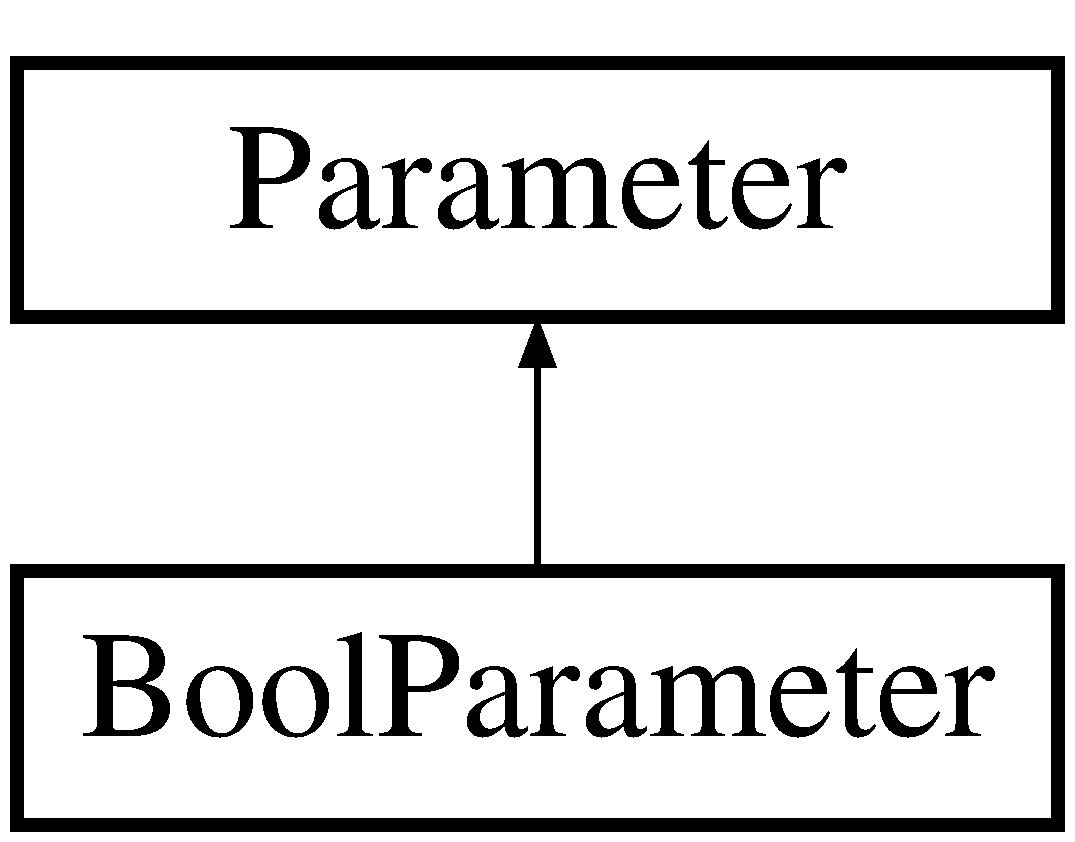
\includegraphics[height=2.000000cm]{classBoolParameter}
\end{center}
\end{figure}
\subsection*{Public Member Functions}
\begin{DoxyCompactItemize}
\item 
\hypertarget{classBoolParameter_afbb5ac0ee11213b125682be7a7bde828}{{\bfseries Bool\-Parameter} (bool value)}\label{classBoolParameter_afbb5ac0ee11213b125682be7a7bde828}

\item 
\hypertarget{classBoolParameter_a361e2d9604deb15e620643803106dabb}{void $\ast$ {\bfseries value} ()}\label{classBoolParameter_a361e2d9604deb15e620643803106dabb}

\end{DoxyCompactItemize}
\subsection*{Additional Inherited Members}


The documentation for this class was generated from the following files\-:\begin{DoxyCompactItemize}
\item 
/home/quentin/\-Projects/\-Asylia/include/core/Parameter.\-hpp\item 
/home/quentin/\-Projects/\-Asylia/source/core/Parameter.\-cpp\end{DoxyCompactItemize}

\hypertarget{classCharacter}{\section{Character Class Reference}
\label{classCharacter}\index{Character@{Character}}
}
Inheritance diagram for Character\-:\begin{figure}[H]
\begin{center}
\leavevmode
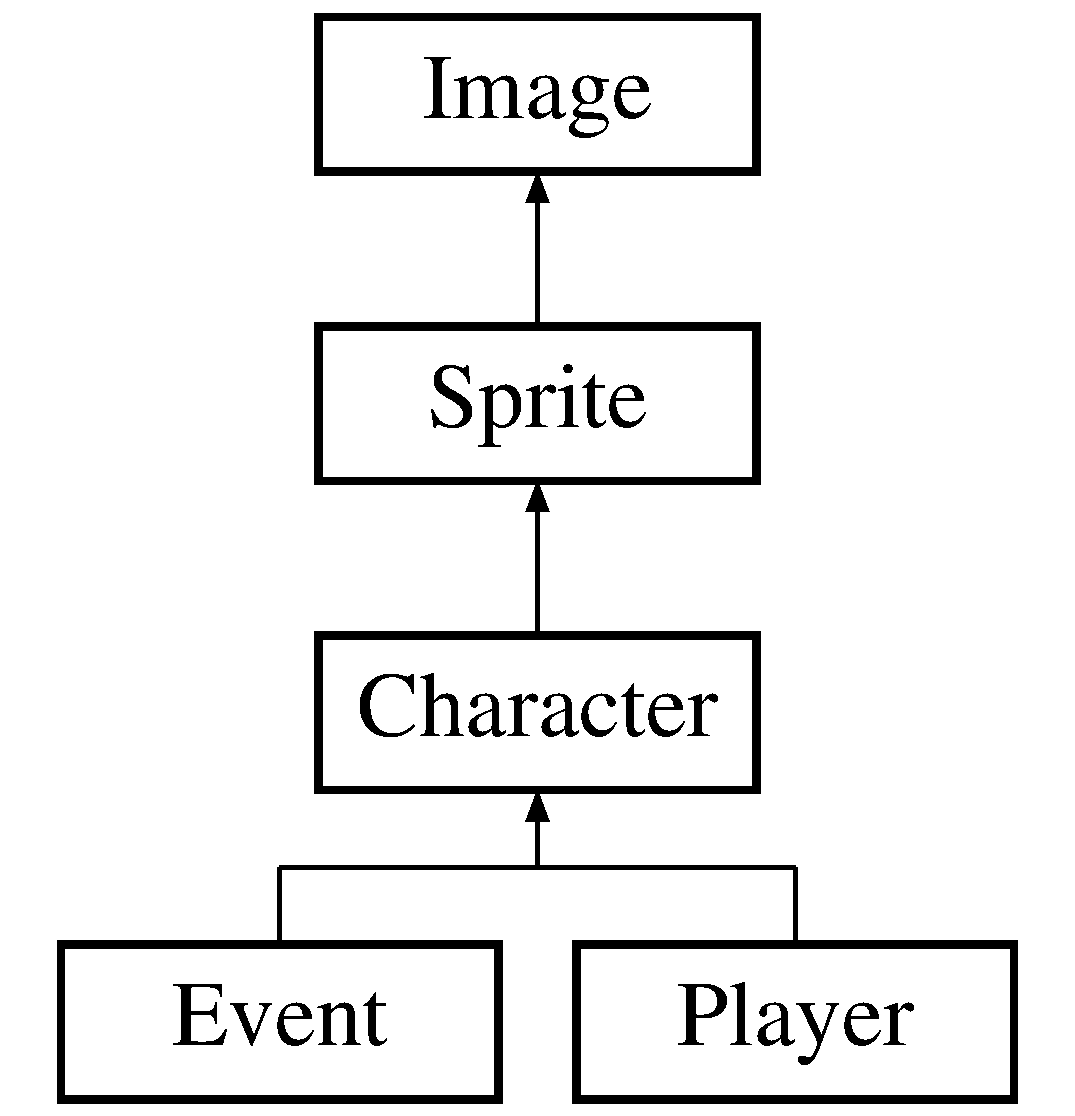
\includegraphics[height=4.000000cm]{classCharacter}
\end{center}
\end{figure}
\subsection*{Public Types}
\begin{DoxyCompactItemize}
\item 
enum {\bfseries Direction} \{ {\bfseries Down}, 
{\bfseries Right}, 
{\bfseries Left}, 
{\bfseries Up}
 \}
\item 
enum {\bfseries Type} \{ {\bfseries None}, 
{\bfseries Player}, 
{\bfseries Type\-N\-P\-C}, 
{\bfseries Type\-Event}
 \}
\end{DoxyCompactItemize}
\subsection*{Public Member Functions}
\begin{DoxyCompactItemize}
\item 
\hypertarget{classCharacter_a2f9e7d0c3b1145a9a921c447f9a3bab7}{{\bfseries Character} (const char $\ast$filename, s16 x, s16 y, u8 direction, u16 frame\-Width=32, u16 frame\-Height=48)}\label{classCharacter_a2f9e7d0c3b1145a9a921c447f9a3bab7}

\item 
\hypertarget{classCharacter_a639f0dfe68079c01cb702073a6451659}{void {\bfseries move} ()}\label{classCharacter_a639f0dfe68079c01cb702073a6451659}

\item 
\hypertarget{classCharacter_aa2026e8ecdbb479eb7bf978575a3a745}{void {\bfseries render} ()}\label{classCharacter_aa2026e8ecdbb479eb7bf978575a3a745}

\item 
\hypertarget{classCharacter_a0f8b3a43420b0fda18d7898bdfca4c2a}{void {\bfseries test\-Collisions} ()}\label{classCharacter_a0f8b3a43420b0fda18d7898bdfca4c2a}

\item 
\hypertarget{classCharacter_a03a3141917ed01abbc72f4c057593bca}{void {\bfseries map\-Collisions} ()}\label{classCharacter_a03a3141917ed01abbc72f4c057593bca}

\item 
\hypertarget{classCharacter_a5462e0c77d02977422aae246ff083005}{void {\bfseries in\-Collision\-With} (\hyperlink{classCharacter}{Character} $\ast$c)}\label{classCharacter_a5462e0c77d02977422aae246ff083005}

\item 
\hypertarget{classCharacter_aed7792d0d0863523c95bd2a888cc8eac}{bool {\bfseries can\-Initiate\-Conversation\-With} (\hyperlink{classCharacter}{Character} $\ast$c)}\label{classCharacter_aed7792d0d0863523c95bd2a888cc8eac}

\item 
\hypertarget{classCharacter_ab8e600ac0238b28f40e67e897fb68ca8}{void {\bfseries event\-Collisions} ()}\label{classCharacter_ab8e600ac0238b28f40e67e897fb68ca8}

\item 
\hypertarget{classCharacter_ab9575098086840989f4bf4565e14513f}{void {\bfseries stop} ()}\label{classCharacter_ab9575098086840989f4bf4565e14513f}

\item 
\hypertarget{classCharacter_ae1e72736b8e8c3f802957e1acfa7ad34}{void {\bfseries collision\-Action} (\hyperlink{classCharacter}{Character} $\ast$c)}\label{classCharacter_ae1e72736b8e8c3f802957e1acfa7ad34}

\item 
\hypertarget{classCharacter_ad967ce11157d1835be0e19873648feeb}{void {\bfseries do\-Movement} (s8 vx, s8 vy)}\label{classCharacter_ad967ce11157d1835be0e19873648feeb}

\item 
\hypertarget{classCharacter_a5e63747ea61305391cd0ada0898e485c}{void {\bfseries move\-Up} ()}\label{classCharacter_a5e63747ea61305391cd0ada0898e485c}

\item 
\hypertarget{classCharacter_afa7763e81bca6a0b9b0c044f39c429f0}{void {\bfseries move\-Down} ()}\label{classCharacter_afa7763e81bca6a0b9b0c044f39c429f0}

\item 
\hypertarget{classCharacter_a88dfc867ab226d3f115b891fc3b34d67}{void {\bfseries move\-Left} ()}\label{classCharacter_a88dfc867ab226d3f115b891fc3b34d67}

\item 
\hypertarget{classCharacter_a0a8bf66e3d70c196a0fa8ce183f4aeb4}{void {\bfseries move\-Right} ()}\label{classCharacter_a0a8bf66e3d70c196a0fa8ce183f4aeb4}

\item 
\hypertarget{classCharacter_a5c474be3ae9a12b416cde56131d6e442}{void {\bfseries change\-Map} (u16 area, u16 map\-X, u16 map\-Y, u16 x, u16 y, u8 direction)}\label{classCharacter_a5c474be3ae9a12b416cde56131d6e442}

\item 
\hypertarget{classCharacter_aaf4ad54e5a10bcbae24c64664e873477}{void {\bfseries gain\-Gold} (u16 value)}\label{classCharacter_aaf4ad54e5a10bcbae24c64664e873477}

\item 
\hypertarget{classCharacter_af7d367c2d38c0c9ee6f821350e7afd4c}{void {\bfseries lose\-Gold} (u16 value)}\label{classCharacter_af7d367c2d38c0c9ee6f821350e7afd4c}

\item 
\hypertarget{classCharacter_a5dbb3462c702f6a9868dece29d45577e}{s16 {\bfseries x} () const }\label{classCharacter_a5dbb3462c702f6a9868dece29d45577e}

\item 
\hypertarget{classCharacter_a08197f0e29e3f9205bb2d222892ace20}{s16 {\bfseries y} () const }\label{classCharacter_a08197f0e29e3f9205bb2d222892ace20}

\item 
\hypertarget{classCharacter_a4565df36ba45828e9a1e8e31ac3688c2}{u8 {\bfseries get\-Direction} () const }\label{classCharacter_a4565df36ba45828e9a1e8e31ac3688c2}

\item 
\hypertarget{classCharacter_a4754500de3c6d9715d7ff736bf1b5554}{void {\bfseries set\-Direction} (u8 direction)}\label{classCharacter_a4754500de3c6d9715d7ff736bf1b5554}

\item 
\hypertarget{classCharacter_a09cb3c5ec8456bb5be06da17672250ce}{void {\bfseries face} (\hyperlink{classCharacter}{Character} $\ast$c)}\label{classCharacter_a09cb3c5ec8456bb5be06da17672250ce}

\item 
\hypertarget{classCharacter_a6000ddb027701dc7d330320bca9c6d42}{bool {\bfseries in\-Front\-Of} (\hyperlink{classCharacter}{Character} $\ast$c)}\label{classCharacter_a6000ddb027701dc7d330320bca9c6d42}

\item 
\hypertarget{classCharacter_a742d70b1552770cac834a713082f5ca4}{void {\bfseries set\-Hitbox} (s16 x, s16 y, u16 width, u16 height)}\label{classCharacter_a742d70b1552770cac834a713082f5ca4}

\item 
\hypertarget{classCharacter_a199cb50dc9add8f5253389db2b8d2f80}{void {\bfseries set\-Position} (s16 x, s16 y)}\label{classCharacter_a199cb50dc9add8f5253389db2b8d2f80}

\item 
\hypertarget{classCharacter_a4fd78979a75d2be44e8d6537789a127f}{\hyperlink{classInventory}{Inventory} $\ast$ {\bfseries inventory} ()}\label{classCharacter_a4fd78979a75d2be44e8d6537789a127f}

\end{DoxyCompactItemize}
\subsection*{Protected Attributes}
\begin{DoxyCompactItemize}
\item 
\hypertarget{classCharacter_a6aaa1409045cb7ce01b572045d082a6a}{Type {\bfseries m\-\_\-type}}\label{classCharacter_a6aaa1409045cb7ce01b572045d082a6a}

\item 
\hypertarget{classCharacter_a94bab35d6f9228f3cd616ddebe2ca569}{u16 {\bfseries m\-\_\-gold}}\label{classCharacter_a94bab35d6f9228f3cd616ddebe2ca569}

\item 
\hypertarget{classCharacter_a12510f0745da930f9565ab0a734708e5}{s16 {\bfseries m\-\_\-x}}\label{classCharacter_a12510f0745da930f9565ab0a734708e5}

\item 
\hypertarget{classCharacter_a1a5f95568f3302a33d581efa4273df04}{s16 {\bfseries m\-\_\-y}}\label{classCharacter_a1a5f95568f3302a33d581efa4273df04}

\item 
\hypertarget{classCharacter_a0e2c0871027ec614f2a7d4e283e9328f}{u8 {\bfseries m\-\_\-direction}}\label{classCharacter_a0e2c0871027ec614f2a7d4e283e9328f}

\item 
\hypertarget{classCharacter_a43300a0a04dbc6dce4d97cd3d4967c51}{s8 {\bfseries m\-\_\-vx}}\label{classCharacter_a43300a0a04dbc6dce4d97cd3d4967c51}

\item 
\hypertarget{classCharacter_a61aa395b3bdfa499f1b32e7ab07b03ef}{s8 {\bfseries m\-\_\-vy}}\label{classCharacter_a61aa395b3bdfa499f1b32e7ab07b03ef}

\item 
\hypertarget{classCharacter_afd4b17ed386481e343d5cc819621e211}{u8 {\bfseries m\-\_\-vx\-Count}}\label{classCharacter_afd4b17ed386481e343d5cc819621e211}

\item 
\hypertarget{classCharacter_aa3dab763ecc28e54e8ffcfd1b67197dc}{u8 {\bfseries m\-\_\-vy\-Count}}\label{classCharacter_aa3dab763ecc28e54e8ffcfd1b67197dc}

\item 
\hypertarget{classCharacter_aab07806fe827950f1b7a20be09b57ab9}{bool {\bfseries m\-\_\-moving}}\label{classCharacter_aab07806fe827950f1b7a20be09b57ab9}

\item 
\hypertarget{classCharacter_ae6caee7127b57536e0e362f8a23eac28}{u8 {\bfseries m\-\_\-speed}}\label{classCharacter_ae6caee7127b57536e0e362f8a23eac28}

\item 
\hypertarget{classCharacter_adf5dd33b7cdbe035eb9d77df092cee2a}{\hyperlink{classTimer}{Timer} {\bfseries m\-\_\-movement\-Timer}}\label{classCharacter_adf5dd33b7cdbe035eb9d77df092cee2a}

\item 
\hypertarget{classCharacter_a285b29a73d9b053012834cb9203bf91d}{u16 {\bfseries m\-\_\-movement\-Delay}}\label{classCharacter_a285b29a73d9b053012834cb9203bf91d}

\item 
\hypertarget{classCharacter_a12dc3a908e7545bdd57b6a0be1026023}{u16 {\bfseries m\-\_\-movement\-I\-D}}\label{classCharacter_a12dc3a908e7545bdd57b6a0be1026023}

\item 
\hypertarget{classCharacter_a62f7fd4c06706d4a7784f0ccc2052fc3}{s16 {\bfseries m\-\_\-hitbox\-X}}\label{classCharacter_a62f7fd4c06706d4a7784f0ccc2052fc3}

\item 
\hypertarget{classCharacter_afe8b09372a17189d666f0b0ea95418da}{s16 {\bfseries m\-\_\-hitbox\-Y}}\label{classCharacter_afe8b09372a17189d666f0b0ea95418da}

\item 
\hypertarget{classCharacter_a65fcf1f2f6c9974fad46d8305d7a9b24}{u16 {\bfseries m\-\_\-hitbox\-W}}\label{classCharacter_a65fcf1f2f6c9974fad46d8305d7a9b24}

\item 
\hypertarget{classCharacter_a69d34ecd6f766d7bcdc109d23bd8fce5}{u16 {\bfseries m\-\_\-hitbox\-H}}\label{classCharacter_a69d34ecd6f766d7bcdc109d23bd8fce5}

\item 
\hypertarget{classCharacter_a7d6dabf9d5e52ae91ede388cfdbc6c4a}{\hyperlink{classCharacter}{Character} $\ast$ {\bfseries m\-\_\-in\-Front\-Of}}\label{classCharacter_a7d6dabf9d5e52ae91ede388cfdbc6c4a}

\item 
\hypertarget{classCharacter_aa923ad7ba7070a25d9722af12188ac7d}{bool {\bfseries m\-\_\-solid}}\label{classCharacter_aa923ad7ba7070a25d9722af12188ac7d}

\item 
\hypertarget{classCharacter_a7eed332ed6050decc2853332df574f4a}{\hyperlink{classInventory}{Inventory} $\ast$ {\bfseries m\-\_\-inventory}}\label{classCharacter_a7eed332ed6050decc2853332df574f4a}

\end{DoxyCompactItemize}


The documentation for this class was generated from the following files\-:\begin{DoxyCompactItemize}
\item 
/home/quentin/\-Projects/\-Asylia/include/entities/Character.\-hpp\item 
/home/quentin/\-Projects/\-Asylia/source/entities/Character.\-cpp\end{DoxyCompactItemize}

\hypertarget{classCharacterManager}{\section{Character\-Manager Class Reference}
\label{classCharacterManager}\index{Character\-Manager@{Character\-Manager}}
}
\subsection*{Static Public Member Functions}
\begin{DoxyCompactItemize}
\item 
\hypertarget{classCharacterManager_a6df9544850a7358a73893eebb40bcffe}{static void {\bfseries init} ()}\label{classCharacterManager_a6df9544850a7358a73893eebb40bcffe}

\item 
\hypertarget{classCharacterManager_ace9949f5f95c9dd0e1a5214f6521a792}{static void {\bfseries free} ()}\label{classCharacterManager_ace9949f5f95c9dd0e1a5214f6521a792}

\item 
\hypertarget{classCharacterManager_a46ce5a4d305031a6c8192ac76394295d}{static void {\bfseries load\-Actors\-Team} ()}\label{classCharacterManager_a46ce5a4d305031a6c8192ac76394295d}

\item 
\hypertarget{classCharacterManager_ad6520b939f17da0de509f8959f98f5f6}{static \hyperlink{classPlayer}{Player} $\ast$ {\bfseries get\-Player} ()}\label{classCharacterManager_ad6520b939f17da0de509f8959f98f5f6}

\end{DoxyCompactItemize}
\subsection*{Static Public Attributes}
\begin{DoxyCompactItemize}
\item 
\hypertarget{classCharacterManager_a92ee7a14dd1ad68b1ffbb5d5b5a627f4}{static \hyperlink{classPlayer}{Player} $\ast$ {\bfseries player} = N\-U\-L\-L}\label{classCharacterManager_a92ee7a14dd1ad68b1ffbb5d5b5a627f4}

\end{DoxyCompactItemize}


The documentation for this class was generated from the following files\-:\begin{DoxyCompactItemize}
\item 
/home/quentin/\-Projects/\-Asylia/include/managers/Character\-Manager.\-hpp\item 
/home/quentin/\-Projects/\-Asylia/source/managers/Character\-Manager.\-cpp\end{DoxyCompactItemize}

\hypertarget{classColor}{\section{Color Class Reference}
\label{classColor}\index{Color@{Color}}
}
\subsection*{Public Member Functions}
\begin{DoxyCompactItemize}
\item 
\hypertarget{classColor_ab6d156688c10e510faa604328d446d67}{{\bfseries Color} (u8 \-\_\-r, u8 \-\_\-g, u8 \-\_\-b, u8 \-\_\-a=255)}\label{classColor_ab6d156688c10e510faa604328d446d67}

\item 
\hypertarget{classColor_a1f89f11d1ed7502e40e1db6611989d2d}{void {\bfseries invert} ()}\label{classColor_a1f89f11d1ed7502e40e1db6611989d2d}

\item 
\hypertarget{classColor_adf897804ed538f1ca0c447f96418cb1c}{\hyperlink{classColor}{Color} {\bfseries operator+} (\hyperlink{classColor}{Color} c)}\label{classColor_adf897804ed538f1ca0c447f96418cb1c}

\end{DoxyCompactItemize}
\subsection*{Public Attributes}
\begin{DoxyCompactItemize}
\item 
\hypertarget{classColor_a72993753060f630faaefc6be380c8254}{u8 {\bfseries r}}\label{classColor_a72993753060f630faaefc6be380c8254}

\item 
\hypertarget{classColor_a832d316e0aacf932d9248e088138ea3b}{u8 {\bfseries g}}\label{classColor_a832d316e0aacf932d9248e088138ea3b}

\item 
\hypertarget{classColor_a51d269461e67faa12c48c3f51bae541a}{u8 {\bfseries b}}\label{classColor_a51d269461e67faa12c48c3f51bae541a}

\item 
\hypertarget{classColor_a3fd865542a4607d9c65a251d60776a89}{u8 {\bfseries a}}\label{classColor_a3fd865542a4607d9c65a251d60776a89}

\end{DoxyCompactItemize}
\subsection*{Static Public Attributes}
\begin{DoxyCompactItemize}
\item 
\hypertarget{classColor_a7257e1adfe8a4a26b1029d5523700410}{static \hyperlink{classColor}{Color} {\bfseries white}}\label{classColor_a7257e1adfe8a4a26b1029d5523700410}

\item 
\hypertarget{classColor_a47086e1bb4d747932c264d53ab570417}{static \hyperlink{classColor}{Color} {\bfseries black}}\label{classColor_a47086e1bb4d747932c264d53ab570417}

\item 
\hypertarget{classColor_a2fbd1aa76c688685adf2b29efffbc8a1}{static \hyperlink{classColor}{Color} {\bfseries system}}\label{classColor_a2fbd1aa76c688685adf2b29efffbc8a1}

\item 
\hypertarget{classColor_a8a69ed9ef0af1289ba995c6c8a0ba027}{static \hyperlink{classColor}{Color} {\bfseries disabled}}\label{classColor_a8a69ed9ef0af1289ba995c6c8a0ba027}

\item 
\hypertarget{classColor_abe661abffec399c494c4d3ff4ae26f83}{static \hyperlink{classColor}{Color} {\bfseries red}}\label{classColor_abe661abffec399c494c4d3ff4ae26f83}

\item 
\hypertarget{classColor_a90dd40fe4beeda39a505c6be65346261}{static \hyperlink{classColor}{Color} {\bfseries green}}\label{classColor_a90dd40fe4beeda39a505c6be65346261}

\end{DoxyCompactItemize}


The documentation for this class was generated from the following files\-:\begin{DoxyCompactItemize}
\item 
/home/quentin/\-Projects/\-Asylia/include/core/Color.\-hpp\item 
/home/quentin/\-Projects/\-Asylia/source/core/Color.\-cpp\end{DoxyCompactItemize}

\hypertarget{classCommandWindow}{\section{Command\-Window Class Reference}
\label{classCommandWindow}\index{Command\-Window@{Command\-Window}}
}
Inheritance diagram for Command\-Window\-:\begin{figure}[H]
\begin{center}
\leavevmode
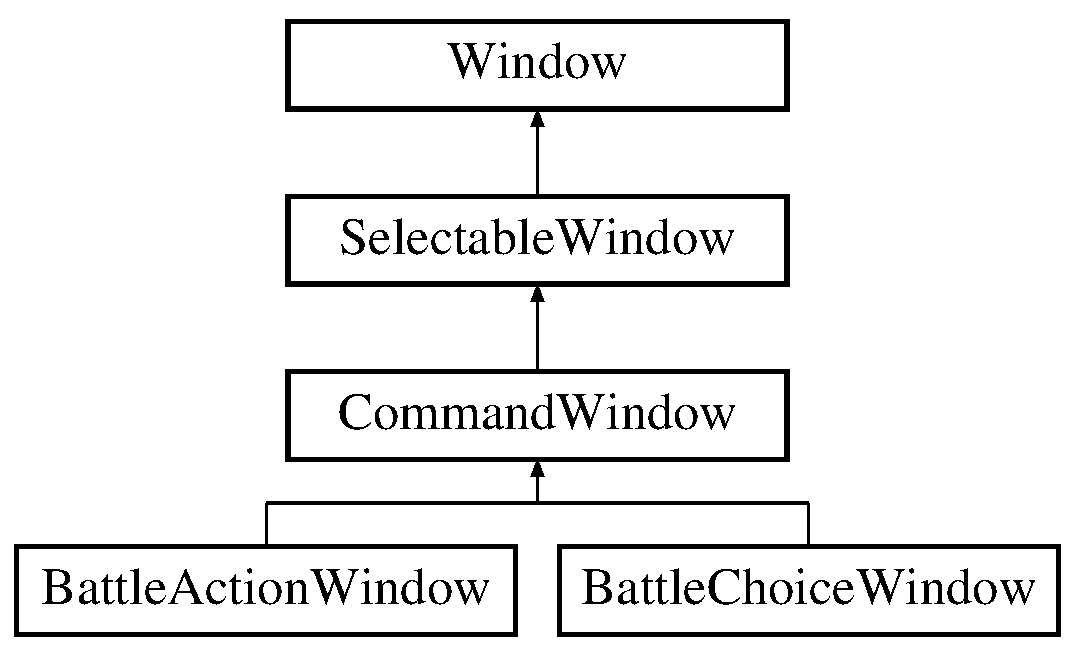
\includegraphics[height=4.000000cm]{classCommandWindow}
\end{center}
\end{figure}
\subsection*{Public Member Functions}
\begin{DoxyCompactItemize}
\item 
\hypertarget{classCommandWindow_a16ce84ea24577933cc9c2b5742858a8e}{{\bfseries Command\-Window} (s16 x, s16 y, u16 width, bool horizontal=false, bool centered=false)}\label{classCommandWindow_a16ce84ea24577933cc9c2b5742858a8e}

\item 
\hypertarget{classCommandWindow_a8dfa172ce7ba6d5b087538956acb6729}{{\bfseries Command\-Window} (u16 width)}\label{classCommandWindow_a8dfa172ce7ba6d5b087538956acb6729}

\item 
\hypertarget{classCommandWindow_a52c2d65f5ac6b625d2818cc04fd3c069}{void {\bfseries clear} ()}\label{classCommandWindow_a52c2d65f5ac6b625d2818cc04fd3c069}

\item 
\hypertarget{classCommandWindow_a25a8dd8239bb0f813b640ae9ade3df42}{void {\bfseries add\-Command} (std\-::string cmd, bool disabled=false)}\label{classCommandWindow_a25a8dd8239bb0f813b640ae9ade3df42}

\item 
\hypertarget{classCommandWindow_ac7010cc621b00bd8e6958f20e8b417a3}{void {\bfseries draw\-Item} (u8 pos)}\label{classCommandWindow_ac7010cc621b00bd8e6958f20e8b417a3}

\item 
\hypertarget{classCommandWindow_a08db648e18e771df8d3e0b1624605b31}{void {\bfseries draw\-Horizontal\-Centered\-Item} (u8 pos)}\label{classCommandWindow_a08db648e18e771df8d3e0b1624605b31}

\item 
\hypertarget{classCommandWindow_a8f7a85f2c08f749325b5989946971c27}{void {\bfseries draw} (bool cursor=true)}\label{classCommandWindow_a8f7a85f2c08f749325b5989946971c27}

\item 
\hypertarget{classCommandWindow_a280a15d609cf66878cc2d729517878e2}{bool {\bfseries disabled} (u8 pos)}\label{classCommandWindow_a280a15d609cf66878cc2d729517878e2}

\item 
\hypertarget{classCommandWindow_af2caf25e22f0113b49103a6a9001eb2d}{std\-::vector$<$ std\-::pair\\*
$<$ std\-::string, bool $>$ $>$ {\bfseries commands} ()}\label{classCommandWindow_af2caf25e22f0113b49103a6a9001eb2d}

\end{DoxyCompactItemize}
\subsection*{Additional Inherited Members}


The documentation for this class was generated from the following files\-:\begin{DoxyCompactItemize}
\item 
/home/quentin/\-Projects/\-Asylia/include/windows/Command\-Window.\-hpp\item 
/home/quentin/\-Projects/\-Asylia/source/windows/Command\-Window.\-cpp\end{DoxyCompactItemize}

\hypertarget{classEndActivity}{\section{End\-Activity Class Reference}
\label{classEndActivity}\index{End\-Activity@{End\-Activity}}
}
Inheritance diagram for End\-Activity\-:\begin{figure}[H]
\begin{center}
\leavevmode
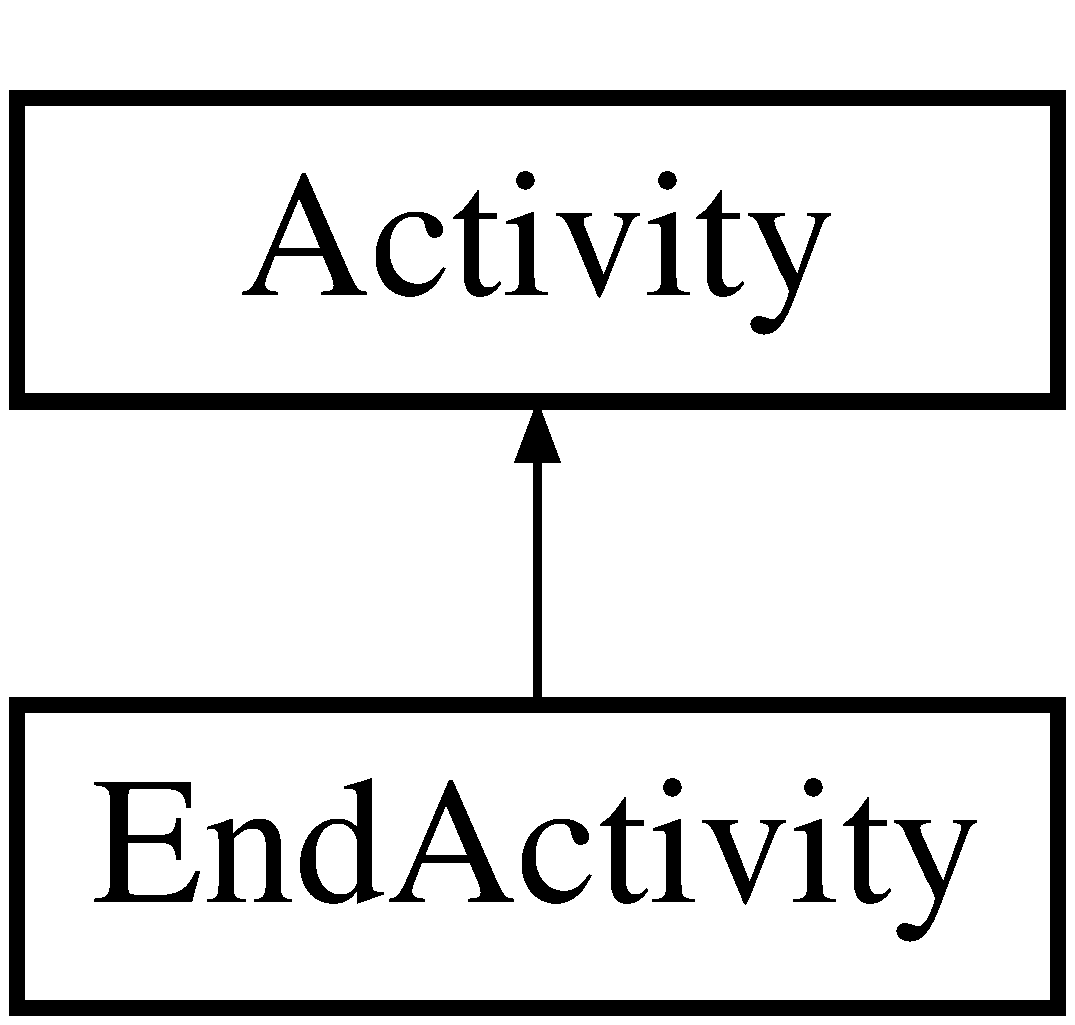
\includegraphics[height=2.000000cm]{classEndActivity}
\end{center}
\end{figure}
\subsection*{Public Member Functions}
\begin{DoxyCompactItemize}
\item 
\hypertarget{classEndActivity_af4e28a8395506f74bbc9f70ac2a987e8}{{\bfseries End\-Activity} (bool disable\-Cancel=false)}\label{classEndActivity_af4e28a8395506f74bbc9f70ac2a987e8}

\item 
\hypertarget{classEndActivity_aa292dbfa6eee70169b4d7df4301990e7}{void {\bfseries update} ()}\label{classEndActivity_aa292dbfa6eee70169b4d7df4301990e7}

\item 
\hypertarget{classEndActivity_a1cf70ac527eb427d60623e8a75307e52}{void {\bfseries render} ()}\label{classEndActivity_a1cf70ac527eb427d60623e8a75307e52}

\end{DoxyCompactItemize}
\subsection*{Additional Inherited Members}


The documentation for this class was generated from the following files\-:\begin{DoxyCompactItemize}
\item 
/home/quentin/\-Projects/\-Asylia/include/activities/End\-Activity.\-hpp\item 
/home/quentin/\-Projects/\-Asylia/source/activities/End\-Activity.\-cpp\end{DoxyCompactItemize}

\hypertarget{classEnemy}{\section{Enemy Class Reference}
\label{classEnemy}\index{Enemy@{Enemy}}
}
Inheritance diagram for Enemy\-:\begin{figure}[H]
\begin{center}
\leavevmode
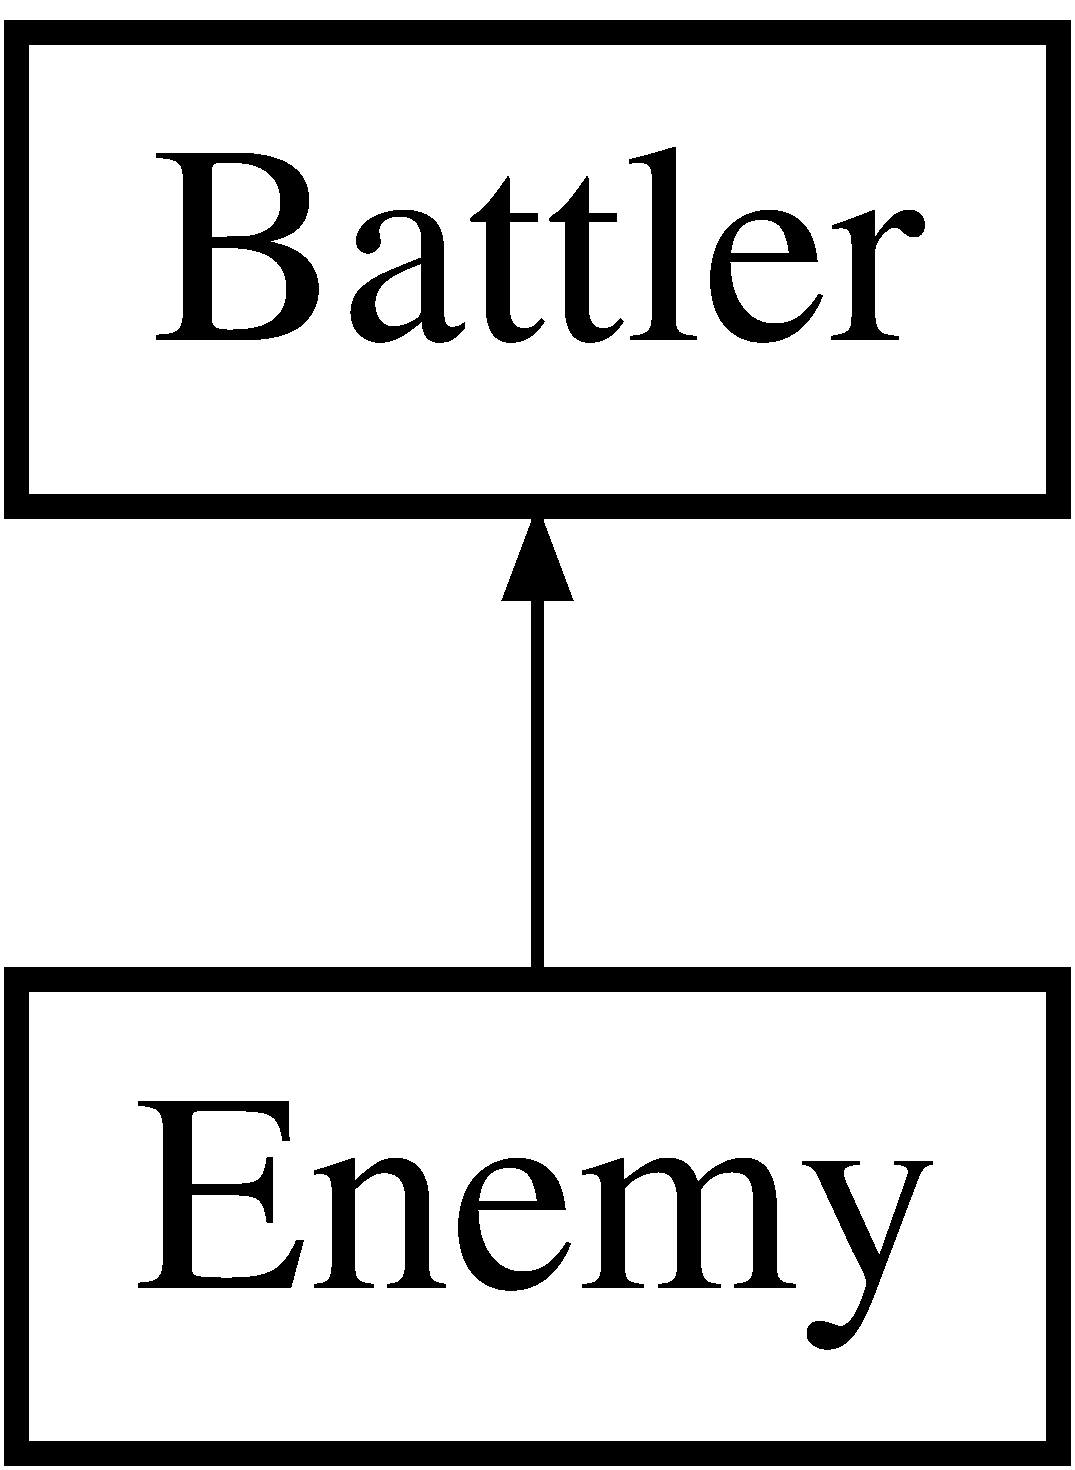
\includegraphics[height=2.000000cm]{classEnemy}
\end{center}
\end{figure}
\subsection*{Public Member Functions}
\begin{DoxyCompactItemize}
\item 
\hypertarget{classEnemy_abf3e5de61b887b9e47968a80e62d1d5d}{{\bfseries Enemy} (std\-::string name, std\-::string appearance, u8 level)}\label{classEnemy_abf3e5de61b887b9e47968a80e62d1d5d}

\item 
\hypertarget{classEnemy_a2043cec6e9e6df1cf75ab2317259bd2a}{std\-::string {\bfseries name} () const }\label{classEnemy_a2043cec6e9e6df1cf75ab2317259bd2a}

\item 
\hypertarget{classEnemy_a79fae600a3aa99ed9b108e0b79d062d5}{\hyperlink{classInventory}{Inventory} $\ast$ {\bfseries loot} ()}\label{classEnemy_a79fae600a3aa99ed9b108e0b79d062d5}

\end{DoxyCompactItemize}
\subsection*{Additional Inherited Members}


The documentation for this class was generated from the following files\-:\begin{DoxyCompactItemize}
\item 
/home/quentin/\-Projects/\-Asylia/include/entities/Enemy.\-hpp\item 
/home/quentin/\-Projects/\-Asylia/source/entities/Enemy.\-cpp\end{DoxyCompactItemize}

\hypertarget{classEquipActivity}{\section{Equip\-Activity Class Reference}
\label{classEquipActivity}\index{Equip\-Activity@{Equip\-Activity}}
}
Inheritance diagram for Equip\-Activity\-:\begin{figure}[H]
\begin{center}
\leavevmode
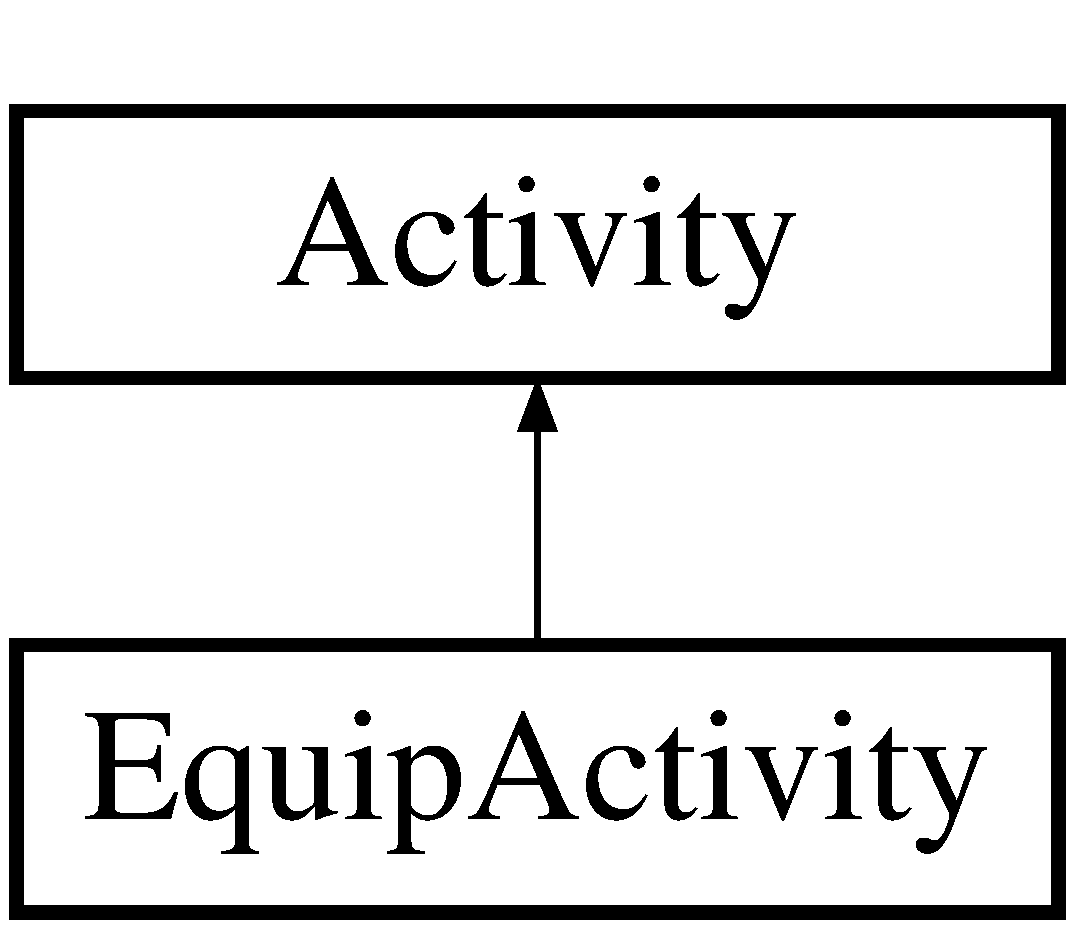
\includegraphics[height=2.000000cm]{classEquipActivity}
\end{center}
\end{figure}
\subsection*{Public Member Functions}
\begin{DoxyCompactItemize}
\item 
\hypertarget{classEquipActivity_a737d1eed35be03426cea3041156513d7}{{\bfseries Equip\-Activity} (u8 actor\-Pos, \hyperlink{classActivity}{Activity} $\ast$parent=N\-U\-L\-L)}\label{classEquipActivity_a737d1eed35be03426cea3041156513d7}

\item 
\hypertarget{classEquipActivity_a436fdca122c478bae6bc576671300302}{void {\bfseries update} ()}\label{classEquipActivity_a436fdca122c478bae6bc576671300302}

\item 
\hypertarget{classEquipActivity_aaac0d2082b216194c7195ad49007dee3}{void {\bfseries render} ()}\label{classEquipActivity_aaac0d2082b216194c7195ad49007dee3}

\item 
\hypertarget{classEquipActivity_a18415dcf81da2c535ed905162c0b7cc2}{bool {\bfseries item\-Mode} () const }\label{classEquipActivity_a18415dcf81da2c535ed905162c0b7cc2}

\item 
\hypertarget{classEquipActivity_a7018ec9ad5ad1bb225e1728029a44b30}{u16 {\bfseries choicewin\-Pos} ()}\label{classEquipActivity_a7018ec9ad5ad1bb225e1728029a44b30}

\end{DoxyCompactItemize}
\subsection*{Additional Inherited Members}


The documentation for this class was generated from the following files\-:\begin{DoxyCompactItemize}
\item 
/home/quentin/\-Projects/\-Asylia/include/activities/Equip\-Activity.\-hpp\item 
/home/quentin/\-Projects/\-Asylia/source/activities/Equip\-Activity.\-cpp\end{DoxyCompactItemize}

\hypertarget{classEquipChoiceWindow}{\section{Equip\-Choice\-Window Class Reference}
\label{classEquipChoiceWindow}\index{Equip\-Choice\-Window@{Equip\-Choice\-Window}}
}
Inheritance diagram for Equip\-Choice\-Window\-:\begin{figure}[H]
\begin{center}
\leavevmode
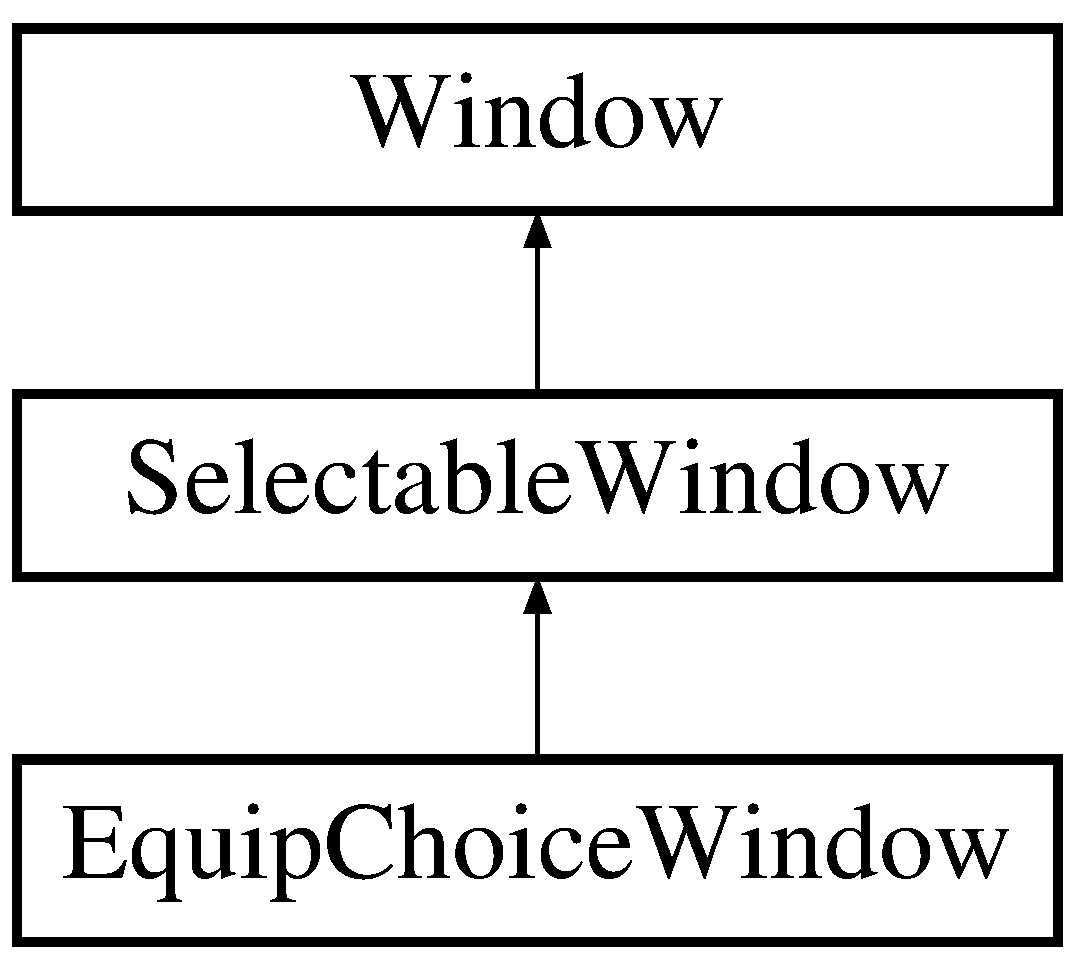
\includegraphics[height=3.000000cm]{classEquipChoiceWindow}
\end{center}
\end{figure}
\subsection*{Public Member Functions}
\begin{DoxyCompactItemize}
\item 
\hypertarget{classEquipChoiceWindow_a2799e91bd5b0ba538e083e60a0294b7e}{{\bfseries Equip\-Choice\-Window} (\hyperlink{classEquipment}{Equipment} $\ast$equipment)}\label{classEquipChoiceWindow_a2799e91bd5b0ba538e083e60a0294b7e}

\item 
\hypertarget{classEquipChoiceWindow_ac57b362baee4ceae21a3e01e1410aeca}{void {\bfseries draw} (bool draw\-Cursor=true)}\label{classEquipChoiceWindow_ac57b362baee4ceae21a3e01e1410aeca}

\end{DoxyCompactItemize}
\subsection*{Additional Inherited Members}


The documentation for this class was generated from the following files\-:\begin{DoxyCompactItemize}
\item 
/home/quentin/\-Projects/\-Asylia/include/windows/Equip\-Choice\-Window.\-hpp\item 
/home/quentin/\-Projects/\-Asylia/source/windows/Equip\-Choice\-Window.\-cpp\end{DoxyCompactItemize}

\hypertarget{classEquipment}{\section{Equipment Class Reference}
\label{classEquipment}\index{Equipment@{Equipment}}
}
\subsection*{Public Member Functions}
\begin{DoxyCompactItemize}
\item 
\hypertarget{classEquipment_a4c9b31ef451a31c0187d61affb7bd594}{void {\bfseries equip\-Weapon} (\hyperlink{classWeapon}{Weapon} $\ast$weapon)}\label{classEquipment_a4c9b31ef451a31c0187d61affb7bd594}

\item 
\hypertarget{classEquipment_a8da617d60d167111c6bfdb386942036e}{void {\bfseries equip\-Armor} (\hyperlink{classArmor}{Armor} $\ast$armor)}\label{classEquipment_a8da617d60d167111c6bfdb386942036e}

\item 
\hypertarget{classEquipment_a71a3feb2a72a0ebbdb96f7f0dda06248}{void {\bfseries unequip\-Weapon} ()}\label{classEquipment_a71a3feb2a72a0ebbdb96f7f0dda06248}

\item 
\hypertarget{classEquipment_aa3f86339d0fbfb19ab9e473a0d1288e1}{void {\bfseries unequip\-Armor} (u8 slot)}\label{classEquipment_aa3f86339d0fbfb19ab9e473a0d1288e1}

\item 
\hypertarget{classEquipment_ab40f07e983d9178710b0f018e3869bf4}{\hyperlink{classWeapon}{Weapon} $\ast$ {\bfseries weapon} () const }\label{classEquipment_ab40f07e983d9178710b0f018e3869bf4}

\item 
\hypertarget{classEquipment_a2950918369da9d2458dc817839da4691}{\hyperlink{classArmor}{Armor} $\ast$ {\bfseries armor} (u8 slot) const }\label{classEquipment_a2950918369da9d2458dc817839da4691}

\item 
\hypertarget{classEquipment_a793475bb4f5eee151711e24f4ec06a5a}{std\-::list$<$ \hyperlink{classArmor}{Armor} $\ast$ $>$ {\bfseries armors} () const }\label{classEquipment_a793475bb4f5eee151711e24f4ec06a5a}

\end{DoxyCompactItemize}


The documentation for this class was generated from the following files\-:\begin{DoxyCompactItemize}
\item 
/home/quentin/\-Projects/\-Asylia/include/objects/Equipment.\-hpp\item 
/home/quentin/\-Projects/\-Asylia/source/objects/Equipment.\-cpp\end{DoxyCompactItemize}

\hypertarget{classEquipStatsWindow}{\section{Equip\-Stats\-Window Class Reference}
\label{classEquipStatsWindow}\index{Equip\-Stats\-Window@{Equip\-Stats\-Window}}
}
Inheritance diagram for Equip\-Stats\-Window\-:\begin{figure}[H]
\begin{center}
\leavevmode
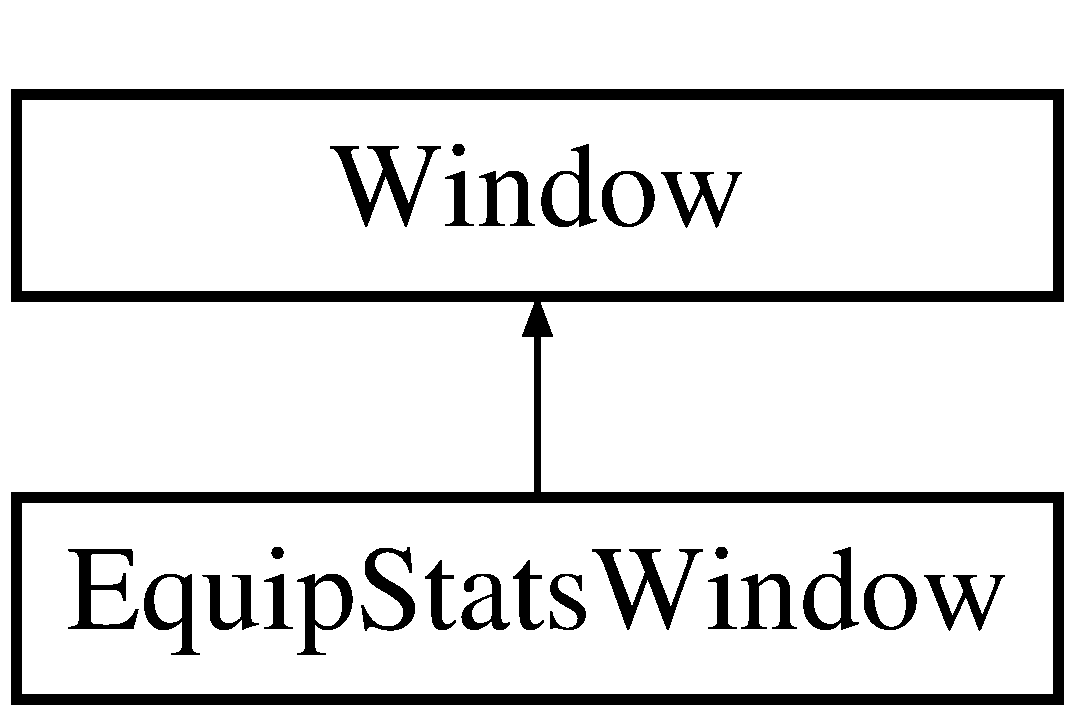
\includegraphics[height=2.000000cm]{classEquipStatsWindow}
\end{center}
\end{figure}
\subsection*{Public Member Functions}
\begin{DoxyCompactItemize}
\item 
\hypertarget{classEquipStatsWindow_a3508019a8b50760ba691cbe35d4c2677}{{\bfseries Equip\-Stats\-Window} (\hyperlink{classActor}{Actor} $\ast$actor)}\label{classEquipStatsWindow_a3508019a8b50760ba691cbe35d4c2677}

\item 
\hypertarget{classEquipStatsWindow_abda3ae8a8a60b3070d77ae7ed0a428df}{void {\bfseries draw} (\hyperlink{classItem}{Item} $\ast$current\-Item=N\-U\-L\-L)}\label{classEquipStatsWindow_abda3ae8a8a60b3070d77ae7ed0a428df}

\end{DoxyCompactItemize}
\subsection*{Additional Inherited Members}


The documentation for this class was generated from the following files\-:\begin{DoxyCompactItemize}
\item 
/home/quentin/\-Projects/\-Asylia/include/windows/Equip\-Stats\-Window.\-hpp\item 
/home/quentin/\-Projects/\-Asylia/source/windows/Equip\-Stats\-Window.\-cpp\end{DoxyCompactItemize}

\hypertarget{classEvent}{\section{Event Class Reference}
\label{classEvent}\index{Event@{Event}}
}
Inheritance diagram for Event\-:\begin{figure}[H]
\begin{center}
\leavevmode
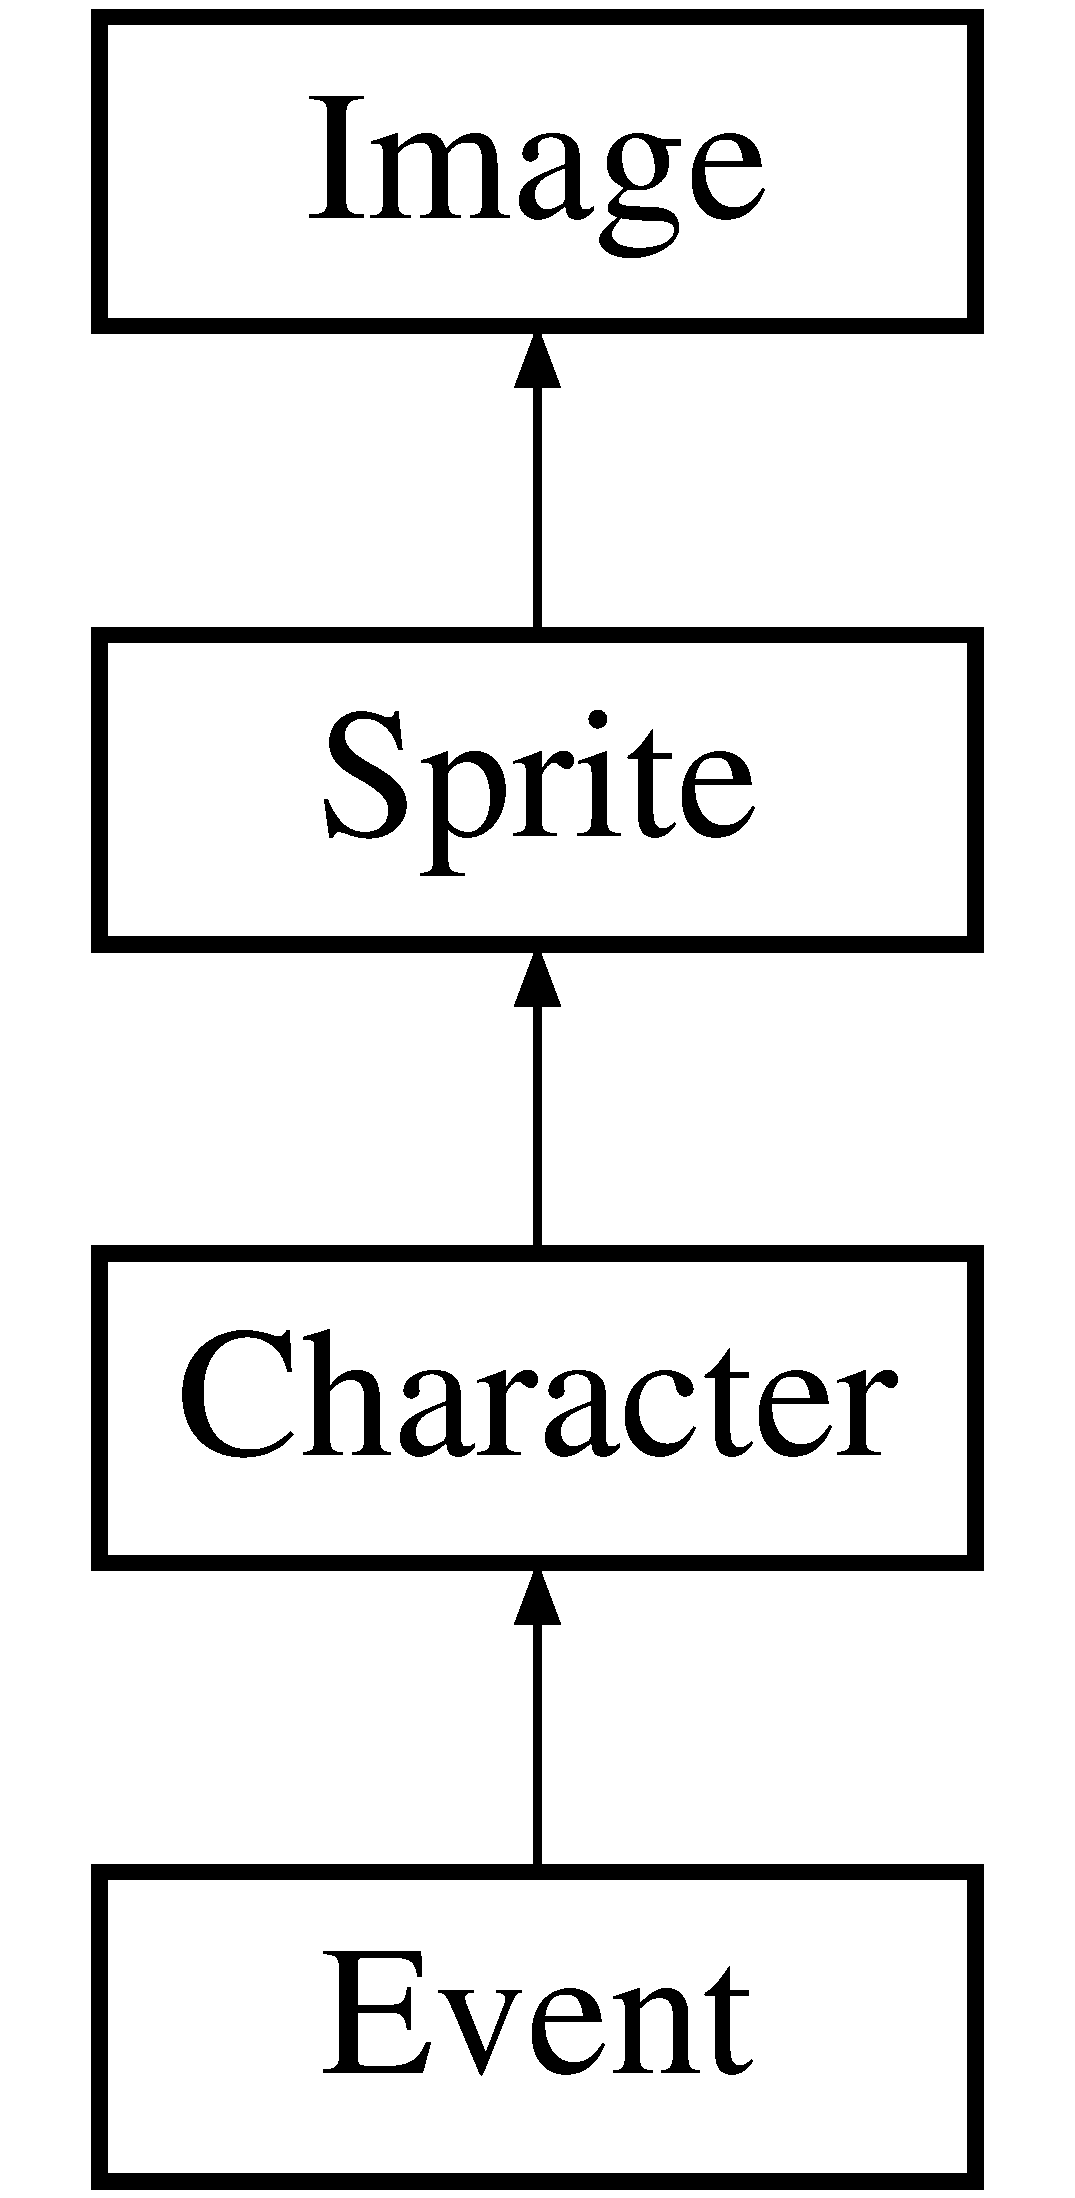
\includegraphics[height=4.000000cm]{classEvent}
\end{center}
\end{figure}
\subsection*{Public Member Functions}
\begin{DoxyCompactItemize}
\item 
\hypertarget{classEvent_af58b43ba8ac202d1ccf3b3f58f33584f}{{\bfseries Event} (std\-::string name, std\-::string appearance, u16 x, u16 y, u8 anim, bool solid=false, u16 frame\-Width=32, u16 frame\-Height=48)}\label{classEvent_af58b43ba8ac202d1ccf3b3f58f33584f}

\item 
\hypertarget{classEvent_a3390735112fadefd4e8850d329471409}{void {\bfseries init} ()}\label{classEvent_a3390735112fadefd4e8850d329471409}

\item 
\hypertarget{classEvent_a844145f6435917f3f37a20c60667441e}{void {\bfseries move} (std\-::string function)}\label{classEvent_a844145f6435917f3f37a20c60667441e}

\item 
\hypertarget{classEvent_a104089a099a45971f10fdf7eaf5654f4}{void {\bfseries update} ()}\label{classEvent_a104089a099a45971f10fdf7eaf5654f4}

\item 
\hypertarget{classEvent_a9ee6473e5e6ccbea302d3f03d1148afd}{void {\bfseries update\-Actions} ()}\label{classEvent_a9ee6473e5e6ccbea302d3f03d1148afd}

\item 
\hypertarget{classEvent_a629a990e09f5ba2b676df218fdb32bf6}{void {\bfseries render} ()}\label{classEvent_a629a990e09f5ba2b676df218fdb32bf6}

\item 
\hypertarget{classEvent_a54b3c3839330abcd2ca796af2565454c}{std\-::string {\bfseries name} () const }\label{classEvent_a54b3c3839330abcd2ca796af2565454c}

\item 
\hypertarget{classEvent_a77ff8a15cc8cdf700a7c86bc680f45aa}{void {\bfseries lock} ()}\label{classEvent_a77ff8a15cc8cdf700a7c86bc680f45aa}

\item 
\hypertarget{classEvent_a3e976db9b1916fb6c64273c4741c76c7}{void {\bfseries unlock} ()}\label{classEvent_a3e976db9b1916fb6c64273c4741c76c7}

\item 
\hypertarget{classEvent_ad8852d64fd863e05c1203a9f94c826ca}{bool {\bfseries is\-Locked} () const }\label{classEvent_ad8852d64fd863e05c1203a9f94c826ca}

\item 
\hypertarget{classEvent_a4a016df82b18e1cfd9d7ab1e0300e51a}{s16 {\bfseries current\-Action\-I\-D} () const }\label{classEvent_a4a016df82b18e1cfd9d7ab1e0300e51a}

\item 
\hypertarget{classEvent_ae428afbb7d64cadd3e3176db9b953646}{void {\bfseries current\-Action\-I\-D} (s16 action\-I\-D)}\label{classEvent_ae428afbb7d64cadd3e3176db9b953646}

\end{DoxyCompactItemize}
\subsection*{Additional Inherited Members}


The documentation for this class was generated from the following files\-:\begin{DoxyCompactItemize}
\item 
/home/quentin/\-Projects/\-Asylia/include/events/Event.\-hpp\item 
/home/quentin/\-Projects/\-Asylia/source/events/Event.\-cpp\end{DoxyCompactItemize}

\hypertarget{classEventAction}{\section{Event\-Action Class Reference}
\label{classEventAction}\index{Event\-Action@{Event\-Action}}
}
\subsection*{Public Member Functions}
\begin{DoxyCompactItemize}
\item 
\hypertarget{classEventAction_aa04ec53a586487c198a3d58000750976}{{\bfseries Event\-Action} (u16 id, u16 action\-Type, \hyperlink{classParameterList}{Parameter\-List} parameters)}\label{classEventAction_aa04ec53a586487c198a3d58000750976}

\item 
\hypertarget{classEventAction_ab70d27d5a2e57786ebe428d912c05133}{u16 {\bfseries id} () const }\label{classEventAction_ab70d27d5a2e57786ebe428d912c05133}

\item 
\hypertarget{classEventAction_a46f890b03c020ea0f9e1f7d2f8afdb7e}{u16 {\bfseries action\-Type} () const }\label{classEventAction_a46f890b03c020ea0f9e1f7d2f8afdb7e}

\item 
\hypertarget{classEventAction_a8268d59c8cb784c79365f958db770567}{\hyperlink{classParameterList}{Parameter\-List} $\ast$ {\bfseries parameters} () const }\label{classEventAction_a8268d59c8cb784c79365f958db770567}

\end{DoxyCompactItemize}


The documentation for this class was generated from the following files\-:\begin{DoxyCompactItemize}
\item 
/home/quentin/\-Projects/\-Asylia/include/events/Event\-Action.\-hpp\item 
/home/quentin/\-Projects/\-Asylia/source/events/Event\-Action.\-cpp\end{DoxyCompactItemize}

\hypertarget{classEventInterpreter}{\section{Event\-Interpreter Class Reference}
\label{classEventInterpreter}\index{Event\-Interpreter@{Event\-Interpreter}}
}
\subsection*{Static Public Member Functions}
\begin{DoxyCompactItemize}
\item 
\hypertarget{classEventInterpreter_ac8a5ac05349eed34424218519a1bbf5c}{static void {\bfseries free} ()}\label{classEventInterpreter_ac8a5ac05349eed34424218519a1bbf5c}

\item 
\hypertarget{classEventInterpreter_a18b1bc95a55713410dc7b3e622d66ff0}{static void {\bfseries add\-Action\-To\-Queue} (u16 id, std\-::string event\-Name, u16 action\-Type, \hyperlink{classParameterList}{Parameter\-List} parameters)}\label{classEventInterpreter_a18b1bc95a55713410dc7b3e622d66ff0}

\item 
\hypertarget{classEventInterpreter_a4b0ea88698556c77d05c92acb95fb54f}{static void {\bfseries update} (\hyperlink{classEvent}{Event} $\ast$e)}\label{classEventInterpreter_a4b0ea88698556c77d05c92acb95fb54f}

\item 
\hypertarget{classEventInterpreter_a413b07b5974e2cae6d153cdc9065b1a9}{static \hyperlink{classParameterList}{Parameter\-List} $\ast$ {\bfseries get\-Parameters} (\hyperlink{classEvent}{Event} $\ast$e)}\label{classEventInterpreter_a413b07b5974e2cae6d153cdc9065b1a9}

\item 
\hypertarget{classEventInterpreter_a81db0b9280b315e3d5efe62cfee6d2af}{static void {\bfseries action0} (\hyperlink{classEvent}{Event} $\ast$e)}\label{classEventInterpreter_a81db0b9280b315e3d5efe62cfee6d2af}

\item 
\hypertarget{classEventInterpreter_adced67617f3cd7521442759ff3b99b3e}{static void {\bfseries action1} (\hyperlink{classEvent}{Event} $\ast$e)}\label{classEventInterpreter_adced67617f3cd7521442759ff3b99b3e}

\item 
\hypertarget{classEventInterpreter_ae734de472b2200e34eea1042c08ec979}{static void {\bfseries action2} (\hyperlink{classEvent}{Event} $\ast$e)}\label{classEventInterpreter_ae734de472b2200e34eea1042c08ec979}

\end{DoxyCompactItemize}
\subsection*{Static Public Attributes}
\begin{DoxyCompactItemize}
\item 
\hypertarget{classEventInterpreter_a239772986bd5ee2baa7e3ca7b23d07e5}{static std\-::map$<$ std\-::string, \\*
std\-::vector$<$ \hyperlink{classEventAction}{Event\-Action} $\ast$ $>$ $>$ {\bfseries actions}}\label{classEventInterpreter_a239772986bd5ee2baa7e3ca7b23d07e5}

\end{DoxyCompactItemize}


The documentation for this class was generated from the following files\-:\begin{DoxyCompactItemize}
\item 
/home/quentin/\-Projects/\-Asylia/include/events/Event\-Interpreter.\-hpp\item 
/home/quentin/\-Projects/\-Asylia/source/events/Event\-Interpreter.\-cpp\end{DoxyCompactItemize}

\hypertarget{classEventManager}{\section{Event\-Manager Class Reference}
\label{classEventManager}\index{Event\-Manager@{Event\-Manager}}
}
\subsection*{Static Public Member Functions}
\begin{DoxyCompactItemize}
\item 
\hypertarget{classEventManager_a62454914f03a84b37f98dd224f2fc435}{static void {\bfseries init} ()}\label{classEventManager_a62454914f03a84b37f98dd224f2fc435}

\item 
\hypertarget{classEventManager_aec7d51c3cc8a14d3975815b959c36df7}{static void {\bfseries free} ()}\label{classEventManager_aec7d51c3cc8a14d3975815b959c36df7}

\item 
\hypertarget{classEventManager_a217e8e0bf1bfb7a5aebe03fa3474e4bf}{static void {\bfseries load\-Libs} ()}\label{classEventManager_a217e8e0bf1bfb7a5aebe03fa3474e4bf}

\item 
\hypertarget{classEventManager_a6def79410e129d3250f938a73dbb76a7}{static void {\bfseries init\-Events} ()}\label{classEventManager_a6def79410e129d3250f938a73dbb76a7}

\item 
\hypertarget{classEventManager_a700c02b50d7715bddc1c42ef46e17839}{static void {\bfseries load\-Character\-Event} (X\-M\-L\-Element $\ast$character\-Element)}\label{classEventManager_a700c02b50d7715bddc1c42ef46e17839}

\item 
\hypertarget{classEventManager_a07bc872ae0f9031938177b0963304fa3}{static void {\bfseries load\-Chest\-Event} (X\-M\-L\-Element $\ast$chest\-Event)}\label{classEventManager_a07bc872ae0f9031938177b0963304fa3}

\item 
\hypertarget{classEventManager_a3881415063eeb5616fad43cbaf9c3ade}{static \hyperlink{classEvent}{Event} $\ast$ {\bfseries get\-Event\-By\-Name} (std\-::string name)}\label{classEventManager_a3881415063eeb5616fad43cbaf9c3ade}

\end{DoxyCompactItemize}
\subsection*{Static Public Attributes}
\begin{DoxyCompactItemize}
\item 
\hypertarget{classEventManager_a284838a41921af7df612b8198b89f0ba}{static std\-::map$<$ std\-::string, \\*
\hyperlink{classEvent}{Event} $\ast$ $>$ {\bfseries events}}\label{classEventManager_a284838a41921af7df612b8198b89f0ba}

\end{DoxyCompactItemize}


The documentation for this class was generated from the following files\-:\begin{DoxyCompactItemize}
\item 
/home/quentin/\-Projects/\-Asylia/include/managers/Event\-Manager.\-hpp\item 
/home/quentin/\-Projects/\-Asylia/source/managers/Event\-Manager.\-cpp\end{DoxyCompactItemize}

\hypertarget{classFloatParameter}{\section{Float\-Parameter Class Reference}
\label{classFloatParameter}\index{Float\-Parameter@{Float\-Parameter}}
}
Inheritance diagram for Float\-Parameter\-:\begin{figure}[H]
\begin{center}
\leavevmode
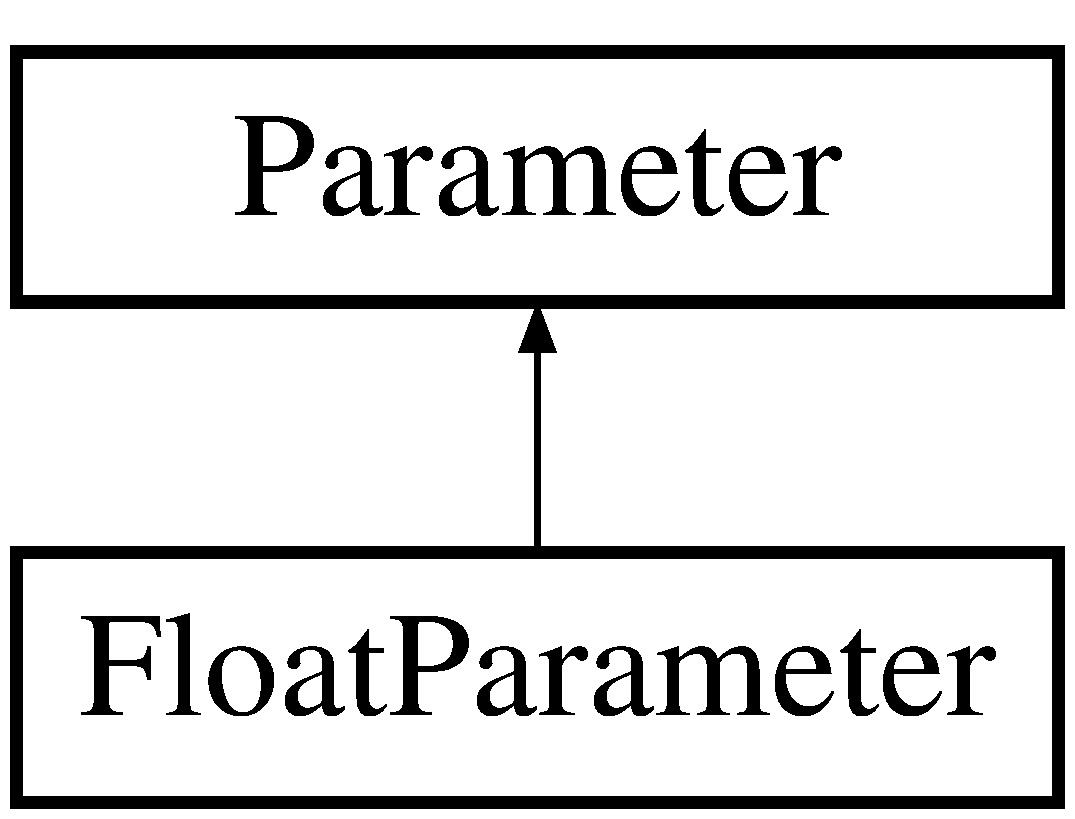
\includegraphics[height=2.000000cm]{classFloatParameter}
\end{center}
\end{figure}
\subsection*{Public Member Functions}
\begin{DoxyCompactItemize}
\item 
\hypertarget{classFloatParameter_aeadaeb2f142c3089523d6a4d8138ceb9}{{\bfseries Float\-Parameter} (float value)}\label{classFloatParameter_aeadaeb2f142c3089523d6a4d8138ceb9}

\item 
\hypertarget{classFloatParameter_a08cacafe82a4539fec410e5a8b2eeede}{void $\ast$ {\bfseries value} ()}\label{classFloatParameter_a08cacafe82a4539fec410e5a8b2eeede}

\end{DoxyCompactItemize}
\subsection*{Additional Inherited Members}


The documentation for this class was generated from the following files\-:\begin{DoxyCompactItemize}
\item 
/home/quentin/\-Projects/\-Asylia/include/core/Parameter.\-hpp\item 
/home/quentin/\-Projects/\-Asylia/source/core/Parameter.\-cpp\end{DoxyCompactItemize}

\hypertarget{classFont}{\section{Font Class Reference}
\label{classFont}\index{Font@{Font}}
}
\subsection*{Public Member Functions}
\begin{DoxyCompactItemize}
\item 
\hypertarget{classFont_af070a503adc8786a2001364db13d1530}{{\bfseries Font} (const char $\ast$filename)}\label{classFont_af070a503adc8786a2001364db13d1530}

\item 
\hypertarget{classFont_a4aaa4551e870bd2fe37e784bd0c50eb4}{void {\bfseries print} (const char $\ast$str, u16 x, u16 y, Font\-Size size, \hyperlink{classColor}{Color} color=Color\-::white)}\label{classFont_a4aaa4551e870bd2fe37e784bd0c50eb4}

\item 
\hypertarget{classFont_a77ed96a1042b358547110d767ca82c9d}{void {\bfseries print\-Scaled} (const char $\ast$str, u16 x, u16 y, u16 width, u16 height, Font\-Size size, \hyperlink{classColor}{Color} color=Color\-::white)}\label{classFont_a77ed96a1042b358547110d767ca82c9d}

\item 
\hypertarget{classFont_ac3649951a4019d1971631e93cacfa012}{void {\bfseries print\-To\-Image} (const char $\ast$str, u16 x, u16 y, \hyperlink{classImage}{Image} $\ast$image, Font\-Size size, \hyperlink{classColor}{Color} color=Color\-::white)}\label{classFont_ac3649951a4019d1971631e93cacfa012}

\item 
\hypertarget{classFont_ac2c1168412d5663f700e341cf813f51e}{void {\bfseries print\-Scaled\-To\-Image} (const char $\ast$str, u16 x, u16 y, u16 width, u16 height, \hyperlink{classImage}{Image} $\ast$image, Font\-Size size, \hyperlink{classColor}{Color} color=Color\-::white)}\label{classFont_ac2c1168412d5663f700e341cf813f51e}

\item 
\hypertarget{classFont_a71b99aa7706cbc7d4fce7cf3b3caef7b}{void {\bfseries print\-Text\-Box} (const char $\ast$str, u16 x, u16 y, u16 width, u16 height, Font\-Size size, \hyperlink{classColor}{Color} color=Color\-::white)}\label{classFont_a71b99aa7706cbc7d4fce7cf3b3caef7b}

\item 
\hypertarget{classFont_a3c8dcee4dd35e8e59bb0789b1ec8aee9}{void {\bfseries print\-Centered} (const char $\ast$str, u16 x, u16 y, u16 width, u16 height, Font\-Size size, \hyperlink{classColor}{Color} color=Color\-::white)}\label{classFont_a3c8dcee4dd35e8e59bb0789b1ec8aee9}

\item 
\hypertarget{classFont_a7e6e9d3b6ed94fc2d7d053a7f1d46263}{void {\bfseries print\-Damages} (u16 damages, u16 x, u16 y, \hyperlink{classColor}{Color} color)}\label{classFont_a7e6e9d3b6ed94fc2d7d053a7f1d46263}

\item 
\hypertarget{classFont_a232096091c450cbee74d35952b480861}{void {\bfseries set\-Style} (Font\-Size size, int style)}\label{classFont_a232096091c450cbee74d35952b480861}

\end{DoxyCompactItemize}


The documentation for this class was generated from the following files\-:\begin{DoxyCompactItemize}
\item 
/home/quentin/\-Projects/\-Asylia/include/display/Font.\-hpp\item 
/home/quentin/\-Projects/\-Asylia/source/display/Font.\-cpp\end{DoxyCompactItemize}

\hypertarget{classGame}{\section{Game Class Reference}
\label{classGame}\index{Game@{Game}}
}
\subsection*{Public Member Functions}
\begin{DoxyCompactItemize}
\item 
\hypertarget{classGame_ae89e277761b7dc5bc7a23fd1b4c6f17d}{void {\bfseries main\-Loop} ()}\label{classGame_ae89e277761b7dc5bc7a23fd1b4c6f17d}

\end{DoxyCompactItemize}
\subsection*{Static Public Attributes}
\begin{DoxyCompactItemize}
\item 
\hypertarget{classGame_ab707809025007494f4cdb1392b56cab9}{static bool {\bfseries quit} = false}\label{classGame_ab707809025007494f4cdb1392b56cab9}

\item 
\hypertarget{classGame_a255049de8fb46a9f00946631e3121c03}{static bool {\bfseries paused} = false}\label{classGame_a255049de8fb46a9f00946631e3121c03}

\end{DoxyCompactItemize}


The documentation for this class was generated from the following files\-:\begin{DoxyCompactItemize}
\item 
/home/quentin/\-Projects/\-Asylia/include/Game.\-hpp\item 
/home/quentin/\-Projects/\-Asylia/source/Game.\-cpp\end{DoxyCompactItemize}

\hypertarget{classGameWindow}{\section{Game\-Window Class Reference}
\label{classGameWindow}\index{Game\-Window@{Game\-Window}}
}
\subsection*{Public Member Functions}
\begin{DoxyCompactItemize}
\item 
\hypertarget{classGameWindow_aa1de835c868c8333dc286e6740b1181a}{{\bfseries Game\-Window} (const char $\ast$caption)}\label{classGameWindow_aa1de835c868c8333dc286e6740b1181a}

\item 
\hypertarget{classGameWindow_afeef7d049b4838c1c112c2be09fe1cd1}{void {\bfseries clear} ()}\label{classGameWindow_afeef7d049b4838c1c112c2be09fe1cd1}

\item 
\hypertarget{classGameWindow_a91e9584fa74547af5f20243bd4a13459}{void {\bfseries update} ()}\label{classGameWindow_a91e9584fa74547af5f20243bd4a13459}

\item 
\hypertarget{classGameWindow_adf76f1d7845fb286d03d68f6a2d3a981}{void {\bfseries set\-Renderer\-Color} (\hyperlink{classColor}{Color} color)}\label{classGameWindow_adf76f1d7845fb286d03d68f6a2d3a981}

\item 
\hypertarget{classGameWindow_aa7cdca538ac9178d7cab420bc40b031b}{void {\bfseries draw\-Rect} (s16 x, s16 y, u16 w, u16 h, \hyperlink{classColor}{Color} c)}\label{classGameWindow_aa7cdca538ac9178d7cab420bc40b031b}

\item 
\hypertarget{classGameWindow_af039273de220d646d7ef889fd91ca23e}{void {\bfseries draw\-Fill\-Rect} (s16 x, s16 y, u16 w, u16 h, \hyperlink{classColor}{Color} c)}\label{classGameWindow_af039273de220d646d7ef889fd91ca23e}

\item 
\hypertarget{classGameWindow_a11f977a749d28dcf778b8fcda71c2930}{S\-D\-L\-\_\-\-Renderer $\ast$ {\bfseries renderer} () const }\label{classGameWindow_a11f977a749d28dcf778b8fcda71c2930}

\item 
\hypertarget{classGameWindow_a40ed07c018823633cd99d06b754a8cc8}{u16 {\bfseries width} () const }\label{classGameWindow_a40ed07c018823633cd99d06b754a8cc8}

\item 
\hypertarget{classGameWindow_a63ecf0a006b298e9785d8aa8b5040cb3}{u16 {\bfseries height} () const }\label{classGameWindow_a63ecf0a006b298e9785d8aa8b5040cb3}

\end{DoxyCompactItemize}
\subsection*{Static Public Attributes}
\begin{DoxyCompactItemize}
\item 
\hypertarget{classGameWindow_a339481fc919a03992d10dd3d2b7d3965}{static \hyperlink{classGameWindow}{Game\-Window} $\ast$ {\bfseries main} = N\-U\-L\-L}\label{classGameWindow_a339481fc919a03992d10dd3d2b7d3965}

\end{DoxyCompactItemize}


The documentation for this class was generated from the following files\-:\begin{DoxyCompactItemize}
\item 
/home/quentin/\-Projects/\-Asylia/include/display/Game\-Window.\-hpp\item 
/home/quentin/\-Projects/\-Asylia/source/display/Game\-Window.\-cpp\end{DoxyCompactItemize}

\hypertarget{classImage}{\section{Image Class Reference}
\label{classImage}\index{Image@{Image}}
}
Inheritance diagram for Image\-:\begin{figure}[H]
\begin{center}
\leavevmode
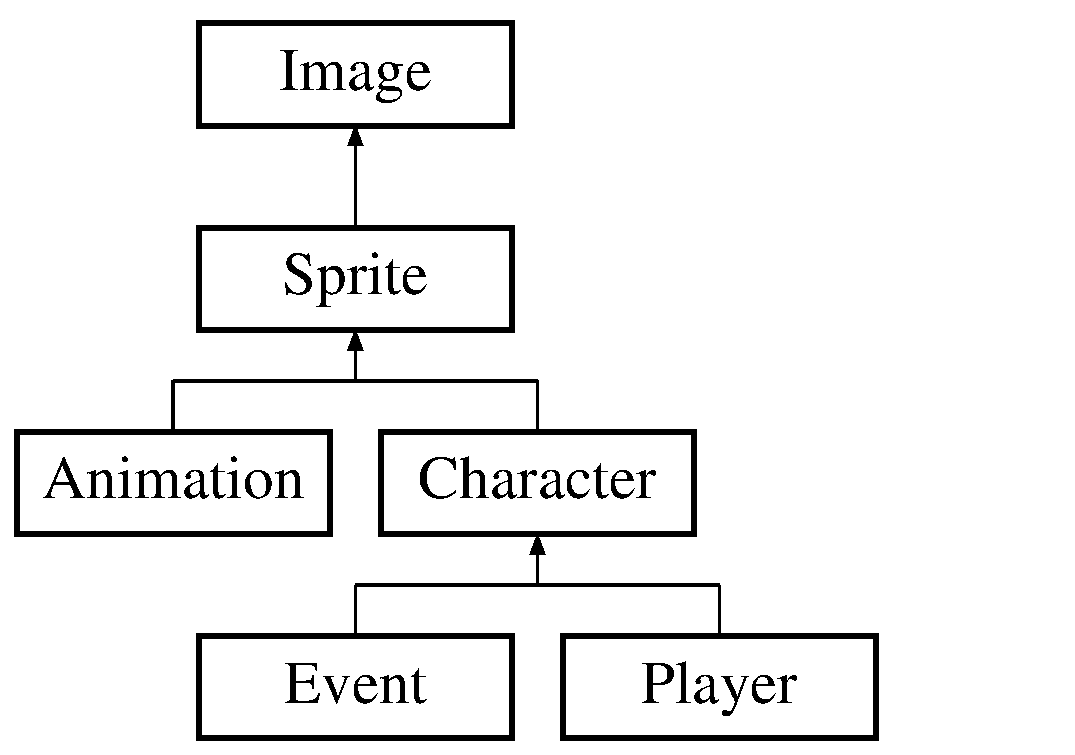
\includegraphics[height=4.000000cm]{classImage}
\end{center}
\end{figure}
\subsection*{Public Member Functions}
\begin{DoxyCompactItemize}
\item 
\hypertarget{classImage_aa44ed77d00d96d2c878b050835f828c4}{{\bfseries Image} (const \hyperlink{classImage}{Image} \&img)}\label{classImage_aa44ed77d00d96d2c878b050835f828c4}

\item 
\hypertarget{classImage_a9700f58efb58b13e23666f19c67d3839}{{\bfseries Image} (const char $\ast$filename)}\label{classImage_a9700f58efb58b13e23666f19c67d3839}

\item 
\hypertarget{classImage_af7e0eee4779e4621a9f6e296800c7d52}{{\bfseries Image} (S\-D\-L\-\_\-\-Surface $\ast$surface)}\label{classImage_af7e0eee4779e4621a9f6e296800c7d52}

\item 
\hypertarget{classImage_a0ca4eb012dd12fdb94ad4dbbe963aae4}{void {\bfseries reload} (const char $\ast$filename)}\label{classImage_a0ca4eb012dd12fdb94ad4dbbe963aae4}

\item 
\hypertarget{classImage_afd1a0b923fbe8db507ed72cf163ddd05}{void {\bfseries reload} (S\-D\-L\-\_\-\-Surface $\ast$surface)}\label{classImage_afd1a0b923fbe8db507ed72cf163ddd05}

\item 
\hypertarget{classImage_a1db998ce4cfeaf7d8ec355b9afe9e823}{void {\bfseries render\-Copy} ()}\label{classImage_a1db998ce4cfeaf7d8ec355b9afe9e823}

\item 
\hypertarget{classImage_afbc635e6974fdf797902f77c5b62848d}{void {\bfseries render} (s16 x=-\/1, s16 y=-\/1, u16 w=0, u16 h=0, s16 clip\-X=-\/1, s16 clip\-Y=-\/1, s16 clip\-W=-\/1, s16 clip\-H=-\/1)}\label{classImage_afbc635e6974fdf797902f77c5b62848d}

\item 
\hypertarget{classImage_a61a65d01ff669ad0cb1221efbcfc679d}{void {\bfseries set\-Pos\-Rect} (s16 x, s16 y, u16 w, u16 h)}\label{classImage_a61a65d01ff669ad0cb1221efbcfc679d}

\item 
\hypertarget{classImage_ad262841ddd13f890ab67032982176bde}{void {\bfseries set\-Clip\-Rect} (s16 x, s16 y, u16 w, u16 h)}\label{classImage_ad262841ddd13f890ab67032982176bde}

\item 
\hypertarget{classImage_a079d3aa6ab7e3160ff1e72c04f3869bb}{void {\bfseries set\-Alpha\-Mod} (u8 alpha)}\label{classImage_a079d3aa6ab7e3160ff1e72c04f3869bb}

\item 
\hypertarget{classImage_a223770f86797fc59b73aa410d0fd6792}{void {\bfseries set\-Color\-Mod} (\hyperlink{classColor}{Color} color)}\label{classImage_a223770f86797fc59b73aa410d0fd6792}

\item 
\hypertarget{classImage_a8e17b43a144137a95c91312173bed741}{std\-::string {\bfseries filename} () const }\label{classImage_a8e17b43a144137a95c91312173bed741}

\item 
\hypertarget{classImage_a6648eeeb998e4d7d4ec963fd9edb2f9a}{u16 {\bfseries width} () const }\label{classImage_a6648eeeb998e4d7d4ec963fd9edb2f9a}

\item 
\hypertarget{classImage_a960cd8de10ae193469eb1becdceb5171}{u16 {\bfseries height} () const }\label{classImage_a960cd8de10ae193469eb1becdceb5171}

\item 
\hypertarget{classImage_a1ccdc88144d49ce5f43ab9a729cae840}{S\-D\-L\-\_\-\-Texture $\ast$ {\bfseries texture} () const }\label{classImage_a1ccdc88144d49ce5f43ab9a729cae840}

\item 
\hypertarget{classImage_a20219efbd6666969756f082ae69f0624}{S\-D\-L\-\_\-\-Rect {\bfseries pos\-Rect} () const }\label{classImage_a20219efbd6666969756f082ae69f0624}

\item 
\hypertarget{classImage_a69de39113107cd56df4a9a937812f433}{bool {\bfseries hidden} () const }\label{classImage_a69de39113107cd56df4a9a937812f433}

\item 
\hypertarget{classImage_a1e62d96f9f2ab2ba5b89c149158025a7}{void {\bfseries hidden} (bool hidden)}\label{classImage_a1e62d96f9f2ab2ba5b89c149158025a7}

\end{DoxyCompactItemize}
\subsection*{Protected Attributes}
\begin{DoxyCompactItemize}
\item 
\hypertarget{classImage_a6dab1b1a50e0abb9db87e3bf7648c430}{std\-::string {\bfseries m\-\_\-filename}}\label{classImage_a6dab1b1a50e0abb9db87e3bf7648c430}

\item 
\hypertarget{classImage_a05be451b89de4970202c7d28f4cd70bb}{u16 {\bfseries m\-\_\-width}}\label{classImage_a05be451b89de4970202c7d28f4cd70bb}

\item 
\hypertarget{classImage_a300eba133fabf9da652e86e7334826d7}{u16 {\bfseries m\-\_\-height}}\label{classImage_a300eba133fabf9da652e86e7334826d7}

\item 
\hypertarget{classImage_a8c659004c835e42f04f6225ab8cb2af7}{S\-D\-L\-\_\-\-Texture $\ast$ {\bfseries m\-\_\-texture}}\label{classImage_a8c659004c835e42f04f6225ab8cb2af7}

\item 
\hypertarget{classImage_a9061dde7d7984463c193ae38f7e1fb3e}{S\-D\-L\-\_\-\-Rect {\bfseries m\-\_\-clip\-Rect}}\label{classImage_a9061dde7d7984463c193ae38f7e1fb3e}

\item 
\hypertarget{classImage_a970cc39a7ac6d2a608e63f080dfc7ff9}{S\-D\-L\-\_\-\-Rect {\bfseries m\-\_\-pos\-Rect}}\label{classImage_a970cc39a7ac6d2a608e63f080dfc7ff9}

\item 
\hypertarget{classImage_a1a2dc74b94194f413b18858b39ac7a50}{bool {\bfseries m\-\_\-hidden}}\label{classImage_a1a2dc74b94194f413b18858b39ac7a50}

\end{DoxyCompactItemize}


The documentation for this class was generated from the following files\-:\begin{DoxyCompactItemize}
\item 
/home/quentin/\-Projects/\-Asylia/include/display/Image.\-hpp\item 
/home/quentin/\-Projects/\-Asylia/source/display/Image.\-cpp\end{DoxyCompactItemize}

\hypertarget{classInfoWindow}{\section{Info\-Window Class Reference}
\label{classInfoWindow}\index{Info\-Window@{Info\-Window}}
}
Inheritance diagram for Info\-Window\-:\begin{figure}[H]
\begin{center}
\leavevmode
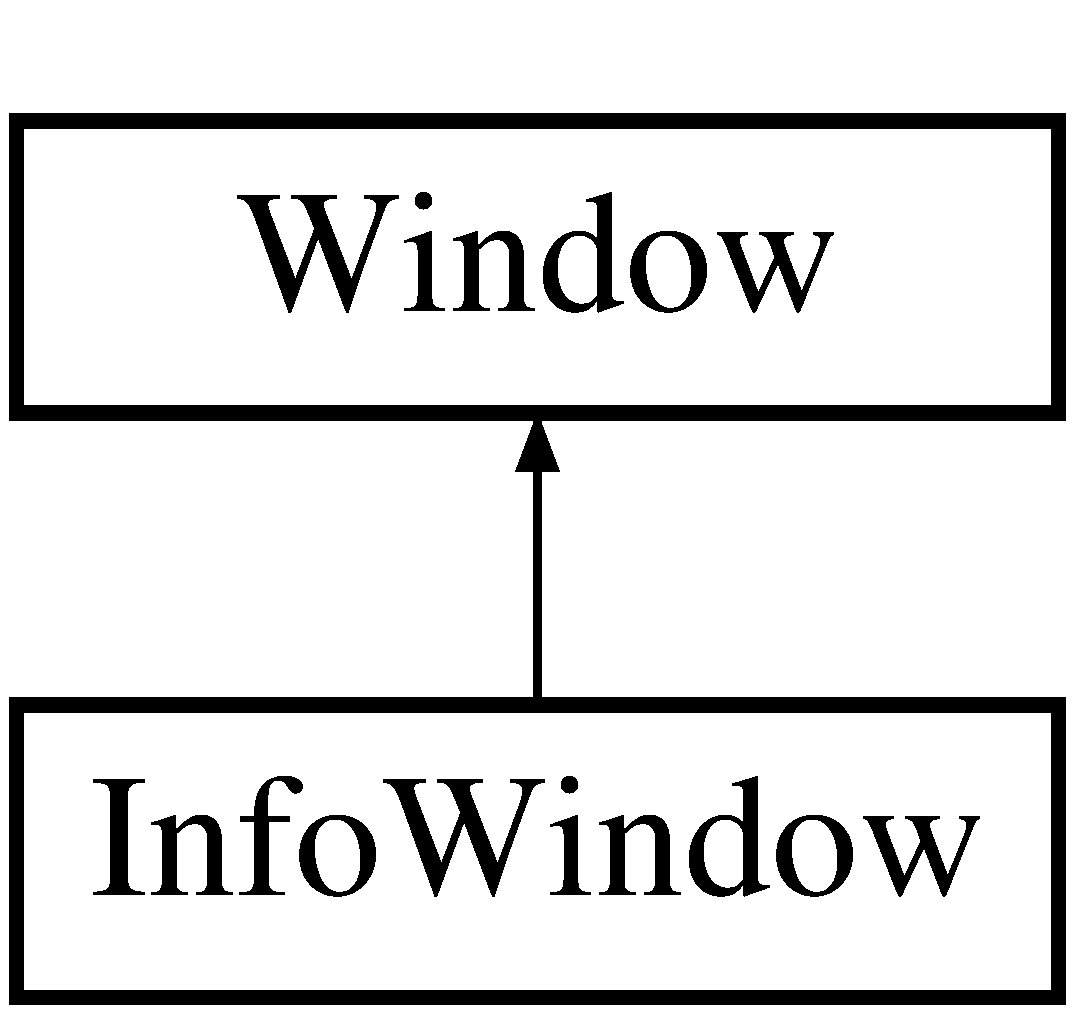
\includegraphics[height=2.000000cm]{classInfoWindow}
\end{center}
\end{figure}
\subsection*{Public Member Functions}
\begin{DoxyCompactItemize}
\item 
\hypertarget{classInfoWindow_abdb33caf040308ccbbcb0628a1745e7b}{{\bfseries Info\-Window} (s16 x, s16 y, u16 width, u16 height)}\label{classInfoWindow_abdb33caf040308ccbbcb0628a1745e7b}

\item 
\hypertarget{classInfoWindow_a198107b7576411592ba2bb9b11578d9b}{void {\bfseries draw\-Text\-Scaled} (std\-::string text)}\label{classInfoWindow_a198107b7576411592ba2bb9b11578d9b}

\item 
\hypertarget{classInfoWindow_a5893404c1f469c98d670cbaeef2a5bdb}{void {\bfseries draw\-Text\-Centered} (std\-::string text)}\label{classInfoWindow_a5893404c1f469c98d670cbaeef2a5bdb}

\end{DoxyCompactItemize}
\subsection*{Additional Inherited Members}


The documentation for this class was generated from the following files\-:\begin{DoxyCompactItemize}
\item 
/home/quentin/\-Projects/\-Asylia/include/windows/Info\-Window.\-hpp\item 
/home/quentin/\-Projects/\-Asylia/source/windows/Info\-Window.\-cpp\end{DoxyCompactItemize}

\hypertarget{classIntParameter}{\section{Int\-Parameter Class Reference}
\label{classIntParameter}\index{Int\-Parameter@{Int\-Parameter}}
}
Inheritance diagram for Int\-Parameter\-:\begin{figure}[H]
\begin{center}
\leavevmode
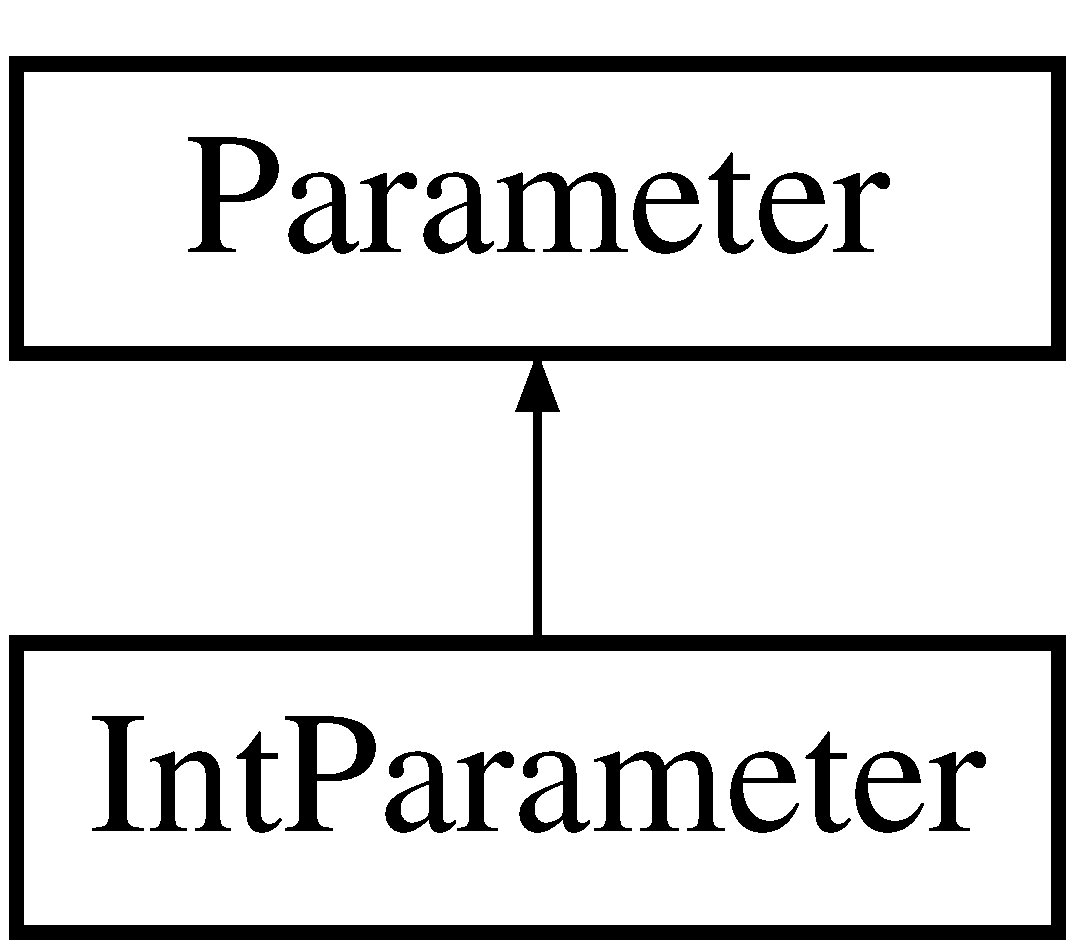
\includegraphics[height=2.000000cm]{classIntParameter}
\end{center}
\end{figure}
\subsection*{Public Member Functions}
\begin{DoxyCompactItemize}
\item 
\hypertarget{classIntParameter_aadb5832cdecc3695e0bc38ac3592c618}{{\bfseries Int\-Parameter} (int value)}\label{classIntParameter_aadb5832cdecc3695e0bc38ac3592c618}

\item 
\hypertarget{classIntParameter_a2a535cb68288e7d5de039d201b84f3e6}{void $\ast$ {\bfseries value} ()}\label{classIntParameter_a2a535cb68288e7d5de039d201b84f3e6}

\end{DoxyCompactItemize}
\subsection*{Additional Inherited Members}


The documentation for this class was generated from the following files\-:\begin{DoxyCompactItemize}
\item 
/home/quentin/\-Projects/\-Asylia/include/core/Parameter.\-hpp\item 
/home/quentin/\-Projects/\-Asylia/source/core/Parameter.\-cpp\end{DoxyCompactItemize}

\hypertarget{classInventory}{\section{Inventory Class Reference}
\label{classInventory}\index{Inventory@{Inventory}}
}
\subsection*{Public Member Functions}
\begin{DoxyCompactItemize}
\item 
\hypertarget{classInventory_a181cdda67bcd1aef95aafe2b7a8432ea}{void {\bfseries clear} ()}\label{classInventory_a181cdda67bcd1aef95aafe2b7a8432ea}

\item 
\hypertarget{classInventory_a075ddcd27c4cb68ca9e2794fc8a176c5}{void {\bfseries add\-Item} (u8 id, s16 count, double chance=1)}\label{classInventory_a075ddcd27c4cb68ca9e2794fc8a176c5}

\item 
\hypertarget{classInventory_a147cb87a117188c995a2223bd14b4bab}{void {\bfseries remove\-Item} (u8 id, s16 count)}\label{classInventory_a147cb87a117188c995a2223bd14b4bab}

\item 
\hypertarget{classInventory_a5367d26bde8ba29070eb2f1fe1430092}{void {\bfseries add\-Armor} (u8 id, s16 count, double chance=1)}\label{classInventory_a5367d26bde8ba29070eb2f1fe1430092}

\item 
\hypertarget{classInventory_aaa5a3f4238d333772d92389d3cc21c57}{void {\bfseries remove\-Armor} (u8 id, s16 count)}\label{classInventory_aaa5a3f4238d333772d92389d3cc21c57}

\item 
\hypertarget{classInventory_ae6d51b42fc94b0674408e2ac4928fde4}{void {\bfseries add\-Weapon} (u8 id, s16 count, double chance=1)}\label{classInventory_ae6d51b42fc94b0674408e2ac4928fde4}

\item 
\hypertarget{classInventory_a70d0469636cbdc17e93179895e22aa97}{void {\bfseries remove\-Weapon} (u8 id, s16 count)}\label{classInventory_a70d0469636cbdc17e93179895e22aa97}

\item 
\hypertarget{classInventory_a093d0530ae59f20c62b13aaf9c1d2e8a}{void {\bfseries add} (\hyperlink{classInventory}{Inventory} $\ast$other, bool with\-Chance=false)}\label{classInventory_a093d0530ae59f20c62b13aaf9c1d2e8a}

\item 
\hypertarget{classInventory_ae207825e3e4ac38293dc91688ad4265e}{u16 {\bfseries nb\-Items} ()}\label{classInventory_ae207825e3e4ac38293dc91688ad4265e}

\item 
\hypertarget{classInventory_a6fbfa8249d45003e19217af040acc608}{u16 {\bfseries nb\-Armors} ()}\label{classInventory_a6fbfa8249d45003e19217af040acc608}

\item 
\hypertarget{classInventory_a073582ba34490cfdd73b6deaeff747da}{u16 {\bfseries nb\-Weapons} ()}\label{classInventory_a073582ba34490cfdd73b6deaeff747da}

\item 
\hypertarget{classInventory_ac8226bbc16088294156ee22421cabb15}{\hyperlink{classItem}{Item} $\ast$ {\bfseries get\-Item} (u16 i)}\label{classInventory_ac8226bbc16088294156ee22421cabb15}

\item 
\hypertarget{classInventory_ab2a6f3ebcb77aafa85b6fba452b7d8b5}{s16 {\bfseries get\-Item\-Count} (u16 i)}\label{classInventory_ab2a6f3ebcb77aafa85b6fba452b7d8b5}

\item 
\hypertarget{classInventory_a3f996724889d568743b0073d647a5c4b}{\hyperlink{classArmor}{Armor} $\ast$ {\bfseries get\-Armor} (u16 i)}\label{classInventory_a3f996724889d568743b0073d647a5c4b}

\item 
\hypertarget{classInventory_aee1c8092f6f9f58537d7ba10d4bd1011}{s16 {\bfseries get\-Armor\-Count} (u16 i)}\label{classInventory_aee1c8092f6f9f58537d7ba10d4bd1011}

\item 
\hypertarget{classInventory_a4559a70df613aedb16f76960cdc60b8f}{\hyperlink{classWeapon}{Weapon} $\ast$ {\bfseries get\-Weapon} (u16 i)}\label{classInventory_a4559a70df613aedb16f76960cdc60b8f}

\item 
\hypertarget{classInventory_a48a6e2a4554f39604ea12fa551e13896}{s16 {\bfseries get\-Weapon\-Count} (u16 i)}\label{classInventory_a48a6e2a4554f39604ea12fa551e13896}

\item 
\hypertarget{classInventory_a080b0370556a8492881e2ca6866a4833}{void {\bfseries push\-Back\-Item} (\hyperlink{classItem}{Item} $\ast$item, s16 count, double chance=1)}\label{classInventory_a080b0370556a8492881e2ca6866a4833}

\item 
\hypertarget{classInventory_a24d0f068e7857fd840a24844442838c4}{std\-::list$<$ std\-::tuple$<$ \hyperlink{classItem}{Item} \\*
$\ast$, s16, double $>$ $>$ {\bfseries items} ()}\label{classInventory_a24d0f068e7857fd840a24844442838c4}

\item 
\hypertarget{classInventory_a74d7902db8cc816e060319b20a2a1c14}{std\-::list$<$ std\-::tuple$<$ \hyperlink{classArmor}{Armor} \\*
$\ast$, s16, double $>$ $>$ {\bfseries armors} ()}\label{classInventory_a74d7902db8cc816e060319b20a2a1c14}

\item 
\hypertarget{classInventory_a8614c96421dfc63a8a8c37237b0c1873}{std\-::list$<$ std\-::tuple$<$ \hyperlink{classWeapon}{Weapon} \\*
$\ast$, s16, double $>$ $>$ {\bfseries weapons} ()}\label{classInventory_a8614c96421dfc63a8a8c37237b0c1873}

\end{DoxyCompactItemize}


The documentation for this class was generated from the following files\-:\begin{DoxyCompactItemize}
\item 
/home/quentin/\-Projects/\-Asylia/include/objects/Inventory.\-hpp\item 
/home/quentin/\-Projects/\-Asylia/source/objects/Inventory.\-cpp\end{DoxyCompactItemize}

\hypertarget{classItem}{\section{Item Class Reference}
\label{classItem}\index{Item@{Item}}
}
Inheritance diagram for Item\-:\begin{figure}[H]
\begin{center}
\leavevmode
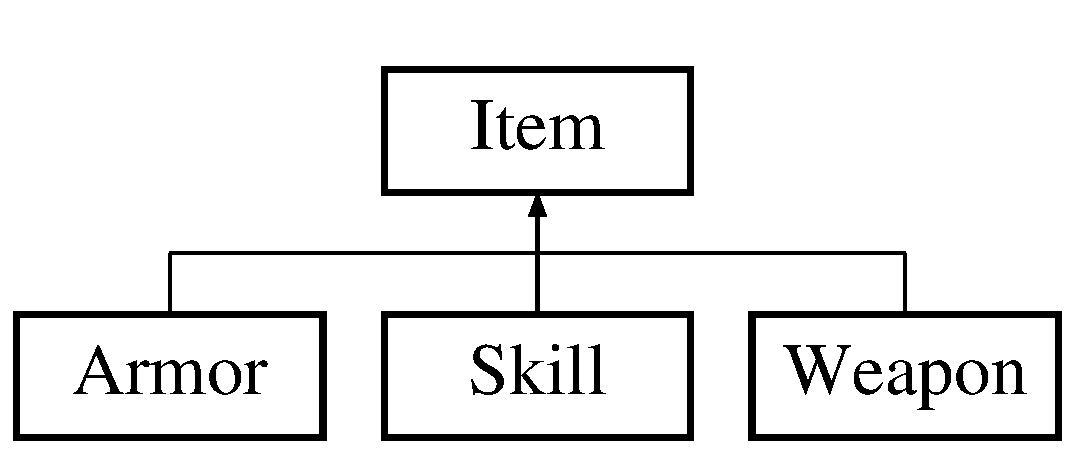
\includegraphics[height=2.000000cm]{classItem}
\end{center}
\end{figure}
\subsection*{Public Types}
\begin{DoxyCompactItemize}
\item 
enum {\bfseries Type} \{ {\bfseries Basic\-Item}, 
{\bfseries Armor}, 
{\bfseries Weapon}, 
{\bfseries Skill}
 \}
\item 
enum {\bfseries Effect} \{ {\bfseries None}, 
{\bfseries Stats\-Effect}, 
{\bfseries Map\-Effect}
 \}
\end{DoxyCompactItemize}
\subsection*{Public Member Functions}
\begin{DoxyCompactItemize}
\item 
\hypertarget{classItem_af8a1515f17080bec7940bdef6afafab5}{{\bfseries Item} (std\-::string name, std\-::string description, std\-::string thumbnail, \hyperlink{classAnimation}{Animation} $\ast$battle\-Animation=N\-U\-L\-L)}\label{classItem_af8a1515f17080bec7940bdef6afafab5}

\item 
\hypertarget{classItem_a151c5fe4902cd18e9b6c626937b4f1be}{u16 {\bfseries id} () const }\label{classItem_a151c5fe4902cd18e9b6c626937b4f1be}

\item 
\hypertarget{classItem_a62d8706352487c714000dfa42fb85153}{std\-::string {\bfseries name} () const }\label{classItem_a62d8706352487c714000dfa42fb85153}

\item 
\hypertarget{classItem_ad0a39f99a07d27ab7722594391e925a4}{std\-::string {\bfseries description} () const }\label{classItem_ad0a39f99a07d27ab7722594391e925a4}

\item 
\hypertarget{classItem_ae30448a5d46a1fb23b9bcde8d69d889e}{u8 {\bfseries level} () const }\label{classItem_ae30448a5d46a1fb23b9bcde8d69d889e}

\item 
\hypertarget{classItem_a1aa25d266f64a06c33bca2cf81c7b788}{\hyperlink{classImage}{Image} $\ast$ {\bfseries thumbnail} () const }\label{classItem_a1aa25d266f64a06c33bca2cf81c7b788}

\item 
\hypertarget{classItem_a52f2ca0ac7fe825e121a9c90143e6c42}{Type {\bfseries type} () const }\label{classItem_a52f2ca0ac7fe825e121a9c90143e6c42}

\item 
\hypertarget{classItem_a351901f73a9053ffb4c9ba8c8f63662b}{Effect {\bfseries effect} () const }\label{classItem_a351901f73a9053ffb4c9ba8c8f63662b}

\item 
\hypertarget{classItem_a245c041c1b2156a4208af87743785454}{\hyperlink{classAnimation}{Animation} $\ast$ {\bfseries battle\-Animation} () const }\label{classItem_a245c041c1b2156a4208af87743785454}

\item 
\hypertarget{classItem_a8173f9b1a560cc3225925fdcd85ea514}{bool {\bfseries equipped} () const }\label{classItem_a8173f9b1a560cc3225925fdcd85ea514}

\item 
\hypertarget{classItem_a91a18049f25e159d961a3bb1c9d89145}{void {\bfseries set\-I\-D} (u16 id)}\label{classItem_a91a18049f25e159d961a3bb1c9d89145}

\item 
\hypertarget{classItem_a0f39e33ed8168d5ebf858b18d8dc989a}{void {\bfseries set\-Effect} (int effect)}\label{classItem_a0f39e33ed8168d5ebf858b18d8dc989a}

\item 
\hypertarget{classItem_a6a09c15d95f8710bd44b1d1a87d206b4}{void {\bfseries set\-Equipped} (bool equipped)}\label{classItem_a6a09c15d95f8710bd44b1d1a87d206b4}

\end{DoxyCompactItemize}
\subsection*{Protected Attributes}
\begin{DoxyCompactItemize}
\item 
\hypertarget{classItem_a1dc38a7820d7a23a4ddcad2a105b571c}{u16 {\bfseries m\-\_\-id}}\label{classItem_a1dc38a7820d7a23a4ddcad2a105b571c}

\item 
\hypertarget{classItem_a7394c7bdb4c682713a8a68bc581b2961}{Type {\bfseries m\-\_\-type}}\label{classItem_a7394c7bdb4c682713a8a68bc581b2961}

\item 
\hypertarget{classItem_a8fb94c83f48fc704f2d03158ad7ccb35}{Effect {\bfseries m\-\_\-effect}}\label{classItem_a8fb94c83f48fc704f2d03158ad7ccb35}

\item 
\hypertarget{classItem_a9f437f59055ce14b5345ccec641d244c}{std\-::string {\bfseries m\-\_\-name}}\label{classItem_a9f437f59055ce14b5345ccec641d244c}

\item 
\hypertarget{classItem_ad86b0caabc1b99000db02358fb94ed17}{std\-::string {\bfseries m\-\_\-description}}\label{classItem_ad86b0caabc1b99000db02358fb94ed17}

\item 
\hypertarget{classItem_ae5c2d96c278ccda3144ad8e894ed9210}{u8 {\bfseries m\-\_\-level}}\label{classItem_ae5c2d96c278ccda3144ad8e894ed9210}

\item 
\hypertarget{classItem_a7104580067c6ccaf7aa2ae886399441b}{\hyperlink{classImage}{Image} $\ast$ {\bfseries m\-\_\-thumbnail}}\label{classItem_a7104580067c6ccaf7aa2ae886399441b}

\item 
\hypertarget{classItem_a928129e5738973ec62b264772448b51a}{\hyperlink{classAnimation}{Animation} $\ast$ {\bfseries m\-\_\-battle\-Animation}}\label{classItem_a928129e5738973ec62b264772448b51a}

\item 
\hypertarget{classItem_aa5b8b59bc839bdd1a9bd835b0fc4e86c}{bool {\bfseries m\-\_\-equipped}}\label{classItem_aa5b8b59bc839bdd1a9bd835b0fc4e86c}

\end{DoxyCompactItemize}


The documentation for this class was generated from the following files\-:\begin{DoxyCompactItemize}
\item 
/home/quentin/\-Projects/\-Asylia/include/objects/Item.\-hpp\item 
/home/quentin/\-Projects/\-Asylia/source/objects/Item.\-cpp\end{DoxyCompactItemize}

\hypertarget{classItemActivity}{\section{Item\-Activity Class Reference}
\label{classItemActivity}\index{Item\-Activity@{Item\-Activity}}
}
Inheritance diagram for Item\-Activity\-:\begin{figure}[H]
\begin{center}
\leavevmode
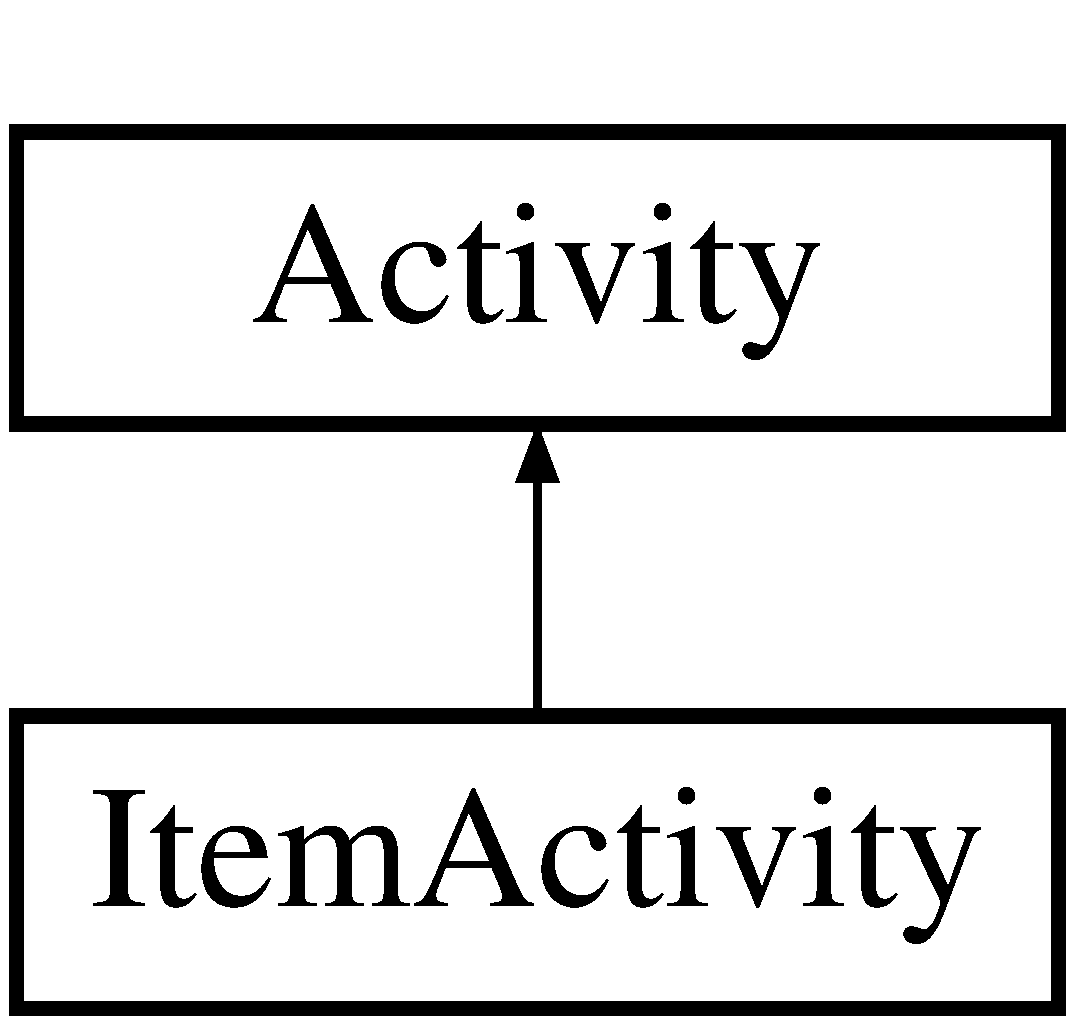
\includegraphics[height=2.000000cm]{classItemActivity}
\end{center}
\end{figure}
\subsection*{Public Member Functions}
\begin{DoxyCompactItemize}
\item 
\hypertarget{classItemActivity_ad3b0d09bac74cba07d8b7c26a58b052f}{{\bfseries Item\-Activity} (\hyperlink{classActivity}{Activity} $\ast$parent=N\-U\-L\-L)}\label{classItemActivity_ad3b0d09bac74cba07d8b7c26a58b052f}

\item 
\hypertarget{classItemActivity_a3008b715c5beb3f9074ba81f466a50d4}{void {\bfseries update} ()}\label{classItemActivity_a3008b715c5beb3f9074ba81f466a50d4}

\item 
\hypertarget{classItemActivity_ae78b5babbc77ceaf4c4a9da199431f7a}{void {\bfseries render} ()}\label{classItemActivity_ae78b5babbc77ceaf4c4a9da199431f7a}

\end{DoxyCompactItemize}
\subsection*{Additional Inherited Members}


The documentation for this class was generated from the following files\-:\begin{DoxyCompactItemize}
\item 
/home/quentin/\-Projects/\-Asylia/include/activities/Item\-Activity.\-hpp\item 
/home/quentin/\-Projects/\-Asylia/source/activities/Item\-Activity.\-cpp\end{DoxyCompactItemize}

\hypertarget{classItemManager}{\section{Item\-Manager Class Reference}
\label{classItemManager}\index{Item\-Manager@{Item\-Manager}}
}
\subsection*{Static Public Member Functions}
\begin{DoxyCompactItemize}
\item 
\hypertarget{classItemManager_a12505eac7fd10a75b1a97ffa7a94468d}{static void {\bfseries init} ()}\label{classItemManager_a12505eac7fd10a75b1a97ffa7a94468d}

\item 
\hypertarget{classItemManager_abd04dfc2ad6abaf81d370f3a93ed2c0d}{static void {\bfseries free} ()}\label{classItemManager_abd04dfc2ad6abaf81d370f3a93ed2c0d}

\item 
\hypertarget{classItemManager_a5dd0f6c4f9b3bf092a958860e1b1e263}{static void {\bfseries load\-Items} ()}\label{classItemManager_a5dd0f6c4f9b3bf092a958860e1b1e263}

\item 
\hypertarget{classItemManager_ac754573383777a828934a947c9321c4b}{static void {\bfseries load\-Armors} ()}\label{classItemManager_ac754573383777a828934a947c9321c4b}

\item 
\hypertarget{classItemManager_a72677ec67e913ce5787f93d7ed3a71e7}{static void {\bfseries load\-Weapons} ()}\label{classItemManager_a72677ec67e913ce5787f93d7ed3a71e7}

\item 
\hypertarget{classItemManager_a52242480e51b5832cbd629aa34bae4c8}{static void {\bfseries load\-Skills} ()}\label{classItemManager_a52242480e51b5832cbd629aa34bae4c8}

\item 
\hypertarget{classItemManager_a5c9224fc3657a2202a91c4e3b195afea}{static \hyperlink{classItem}{Item} $\ast$ {\bfseries get\-Item} (u16 id)}\label{classItemManager_a5c9224fc3657a2202a91c4e3b195afea}

\item 
\hypertarget{classItemManager_a075f63e61a236fe7fbb806c2c50c53e9}{static \hyperlink{classArmor}{Armor} $\ast$ {\bfseries get\-Armor} (u16 id)}\label{classItemManager_a075f63e61a236fe7fbb806c2c50c53e9}

\item 
\hypertarget{classItemManager_a3be27a37c758c0bc2fcfa662571bfabc}{static \hyperlink{classWeapon}{Weapon} $\ast$ {\bfseries get\-Weapon} (u16 id)}\label{classItemManager_a3be27a37c758c0bc2fcfa662571bfabc}

\item 
\hypertarget{classItemManager_a712fe562ca6ee14ceda5a90eb58c873f}{static \hyperlink{classSkill}{Skill} $\ast$ {\bfseries get\-Skill} (u16 id)}\label{classItemManager_a712fe562ca6ee14ceda5a90eb58c873f}

\end{DoxyCompactItemize}
\subsection*{Static Public Attributes}
\begin{DoxyCompactItemize}
\item 
\hypertarget{classItemManager_aabf6d12187715764bfb451c7e947d472}{static std\-::vector$<$ \hyperlink{classItem}{Item} $\ast$ $>$ {\bfseries items}}\label{classItemManager_aabf6d12187715764bfb451c7e947d472}

\item 
\hypertarget{classItemManager_ad00daeaa0bcfb306ef7ec2fe9fdc3850}{static std\-::vector$<$ \hyperlink{classArmor}{Armor} $\ast$ $>$ {\bfseries armors}}\label{classItemManager_ad00daeaa0bcfb306ef7ec2fe9fdc3850}

\item 
\hypertarget{classItemManager_aa62d65473c44e892eb48aca3d72e634f}{static std\-::vector$<$ \hyperlink{classWeapon}{Weapon} $\ast$ $>$ {\bfseries weapons}}\label{classItemManager_aa62d65473c44e892eb48aca3d72e634f}

\item 
\hypertarget{classItemManager_a20fceaafe023d5d6073f37afe3859cca}{static std\-::vector$<$ \hyperlink{classSkill}{Skill} $\ast$ $>$ {\bfseries skills}}\label{classItemManager_a20fceaafe023d5d6073f37afe3859cca}

\end{DoxyCompactItemize}


The documentation for this class was generated from the following files\-:\begin{DoxyCompactItemize}
\item 
/home/quentin/\-Projects/\-Asylia/include/objects/Item\-Manager.\-hpp\item 
/home/quentin/\-Projects/\-Asylia/source/managers/Item\-Manager.\-cpp\end{DoxyCompactItemize}

\hypertarget{classItemWindow}{\section{Item\-Window Class Reference}
\label{classItemWindow}\index{Item\-Window@{Item\-Window}}
}
Inheritance diagram for Item\-Window\-:\begin{figure}[H]
\begin{center}
\leavevmode
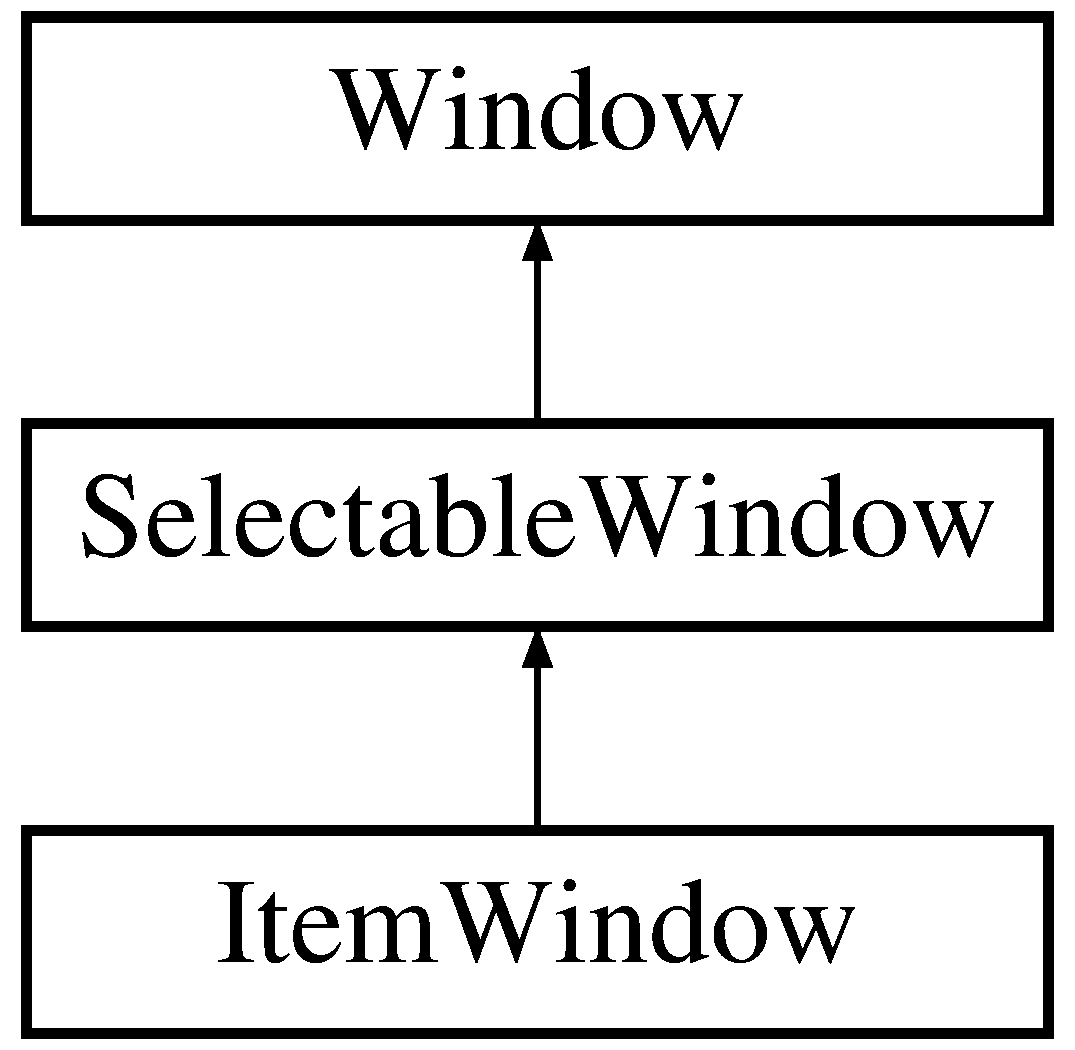
\includegraphics[height=3.000000cm]{classItemWindow}
\end{center}
\end{figure}
\subsection*{Public Member Functions}
\begin{DoxyCompactItemize}
\item 
\hypertarget{classItemWindow_a23f76769ab7374f40a1d4b45180e492c}{{\bfseries Item\-Window} (s16 x, s16 y, u16 width, u16 height, \hyperlink{classInventory}{Inventory} $\ast$inventory, s16 infowin\-X=0, s16 infowin\-Y=0)}\label{classItemWindow_a23f76769ab7374f40a1d4b45180e492c}

\item 
\hypertarget{classItemWindow_a77d161b9abee9e5afd4116fee24c0bd3}{void {\bfseries draw\-Item} (u8 pos)}\label{classItemWindow_a77d161b9abee9e5afd4116fee24c0bd3}

\item 
\hypertarget{classItemWindow_aaebbeb39fd0130eb137b11a593ea9740}{void {\bfseries draw} (bool cursor=true, bool info\-Win\-Text=true)}\label{classItemWindow_aaebbeb39fd0130eb137b11a593ea9740}

\item 
\hypertarget{classItemWindow_a5ea243b742a868a13a1c26cf0e43b523}{void {\bfseries change\-Set} (u8 equip\-I\-D, u8 equip\-Type, \hyperlink{classEquipment}{Equipment} $\ast$equipment)}\label{classItemWindow_a5ea243b742a868a13a1c26cf0e43b523}

\item 
\hypertarget{classItemWindow_a2e20d76641d8fc050c35bdceb11c1271}{bool {\bfseries has\-Items} ()}\label{classItemWindow_a2e20d76641d8fc050c35bdceb11c1271}

\item 
\hypertarget{classItemWindow_af397b141803171fc3e4cdb8fc71da1ca}{\hyperlink{classItem}{Item} $\ast$ {\bfseries current\-Item} ()}\label{classItemWindow_af397b141803171fc3e4cdb8fc71da1ca}

\end{DoxyCompactItemize}
\subsection*{Additional Inherited Members}


The documentation for this class was generated from the following files\-:\begin{DoxyCompactItemize}
\item 
/home/quentin/\-Projects/\-Asylia/include/windows/Item\-Window.\-hpp\item 
/home/quentin/\-Projects/\-Asylia/source/windows/Item\-Window.\-cpp\end{DoxyCompactItemize}

\hypertarget{classKeyboard}{\section{Keyboard Class Reference}
\label{classKeyboard}\index{Keyboard@{Keyboard}}
}
\subsection*{Static Public Member Functions}
\begin{DoxyCompactItemize}
\item 
\hypertarget{classKeyboard_ae75418ec058c9faa11da8a00600debf0}{static const u8 $\ast$ {\bfseries get\-State} ()}\label{classKeyboard_ae75418ec058c9faa11da8a00600debf0}

\item 
\hypertarget{classKeyboard_a6410f07ddc53561a82d5328d8b330aab}{static void {\bfseries update} ()}\label{classKeyboard_a6410f07ddc53561a82d5328d8b330aab}

\item 
\hypertarget{classKeyboard_a9335bbe850023636c516fd3097b80682}{static void {\bfseries force\-Update} ()}\label{classKeyboard_a9335bbe850023636c516fd3097b80682}

\item 
\hypertarget{classKeyboard_acec5b8eed39c370d54f8a37f836599eb}{static void {\bfseries reset\-Pad} (S\-D\-L\-\_\-\-Event $\ast$e, bool released=false)}\label{classKeyboard_acec5b8eed39c370d54f8a37f836599eb}

\item 
\hypertarget{classKeyboard_a28b59927237e9ca52cd30a1f6edcd543}{static void {\bfseries update\-Pad} (S\-D\-L\-\_\-\-Event $\ast$e)}\label{classKeyboard_a28b59927237e9ca52cd30a1f6edcd543}

\item 
\hypertarget{classKeyboard_a9b181f95b0743003ac6ddefa4d2ac788}{static bool {\bfseries is\-Key\-Pressed} (u32 key)}\label{classKeyboard_a9b181f95b0743003ac6ddefa4d2ac788}

\item 
\hypertarget{classKeyboard_a4be9c375121e8de66e858b2b2f01cd5f}{static bool {\bfseries is\-Key\-Pressed\-Once} (u32 key)}\label{classKeyboard_a4be9c375121e8de66e858b2b2f01cd5f}

\item 
\hypertarget{classKeyboard_a5a39520afd20c574bf3d574069005449}{static bool {\bfseries is\-Key\-Pressed\-With\-Delay} (u32 key, u16 delay)}\label{classKeyboard_a5a39520afd20c574bf3d574069005449}

\end{DoxyCompactItemize}
\subsection*{Static Public Attributes}
\begin{DoxyCompactItemize}
\item 
\hypertarget{classKeyboard_a08007721b0a4fd6e9f7cfe28c70642f7}{static const u8 $\ast$ {\bfseries state} = N\-U\-L\-L}\label{classKeyboard_a08007721b0a4fd6e9f7cfe28c70642f7}

\item 
\hypertarget{classKeyboard_a06624a2a2b9d99013c2a8628e987b616}{static u8 {\bfseries pad\-State} \mbox{[}7\mbox{]} = \{0, 0, 0, 0, 0, 0, 0\}}\label{classKeyboard_a06624a2a2b9d99013c2a8628e987b616}

\item 
\hypertarget{classKeyboard_a9bf5466f6c1ff2e61083f338adada94a}{static s32 {\bfseries pad\-Finger} \mbox{[}7\mbox{]} = \{-\/1, -\/1, -\/1, -\/1, -\/1, -\/1, -\/1\}}\label{classKeyboard_a9bf5466f6c1ff2e61083f338adada94a}

\item 
\hypertarget{classKeyboard_a737a295b7ba6d914fde38f161c86c6eb}{static u32 {\bfseries last\-Time\-Pressed} \mbox{[}7\mbox{]} = \{0, 0, 0, 0, 0, 0, 0\}}\label{classKeyboard_a737a295b7ba6d914fde38f161c86c6eb}

\item 
\hypertarget{classKeyboard_a7be1de7dabf081e6d8a6999976fcce14}{static u8 {\bfseries pressed} \mbox{[}7\mbox{]} = \{0, 0, 0, 0, 0, 0, 0\}}\label{classKeyboard_a7be1de7dabf081e6d8a6999976fcce14}

\item 
static u32 {\bfseries keys\-Code} \mbox{[}7\mbox{]}
\item 
\hypertarget{classKeyboard_aed71247c8acfe01b6ef9199fcb8fb9f7}{static const u32 {\bfseries Game\-Up} = P\-A\-D\-\_\-\-U\-P}\label{classKeyboard_aed71247c8acfe01b6ef9199fcb8fb9f7}

\item 
\hypertarget{classKeyboard_af40e4943fa960c4a09a9e835a32662c0}{static const u32 {\bfseries Game\-Down} = P\-A\-D\-\_\-\-D\-O\-W\-N}\label{classKeyboard_af40e4943fa960c4a09a9e835a32662c0}

\item 
\hypertarget{classKeyboard_a70832e4a44d3d57886fcd9f9946557d2}{static const u32 {\bfseries Game\-Left} = P\-A\-D\-\_\-\-L\-E\-F\-T}\label{classKeyboard_a70832e4a44d3d57886fcd9f9946557d2}

\item 
\hypertarget{classKeyboard_ac802f359882ec1a1cb973c0c2ea4cf33}{static const u32 {\bfseries Game\-Right} = P\-A\-D\-\_\-\-R\-I\-G\-H\-T}\label{classKeyboard_ac802f359882ec1a1cb973c0c2ea4cf33}

\item 
\hypertarget{classKeyboard_a57b7df9b59dc8f0d236bdcb31cd6218a}{static const u32 {\bfseries Game\-Attack} = P\-A\-D\-\_\-\-A}\label{classKeyboard_a57b7df9b59dc8f0d236bdcb31cd6218a}

\item 
\hypertarget{classKeyboard_a54e2a9e16cf0abc68a69fb55747faac5}{static const u32 {\bfseries Game\-Back} = P\-A\-D\-\_\-\-B}\label{classKeyboard_a54e2a9e16cf0abc68a69fb55747faac5}

\item 
\hypertarget{classKeyboard_a10b9fae028e00cc0c20aa63f420f9ebc}{static const u32 {\bfseries Game\-Menu} = P\-A\-D\-\_\-\-M\-E\-N\-U}\label{classKeyboard_a10b9fae028e00cc0c20aa63f420f9ebc}

\end{DoxyCompactItemize}


\subsection{Member Data Documentation}
\hypertarget{classKeyboard_ae7ca0673df6ed9edf8bbb15dc4a75e90}{\index{Keyboard@{Keyboard}!keys\-Code@{keys\-Code}}
\index{keys\-Code@{keys\-Code}!Keyboard@{Keyboard}}
\subsubsection[{keys\-Code}]{\setlength{\rightskip}{0pt plus 5cm}u32 Keyboard\-::keys\-Code\hspace{0.3cm}{\ttfamily [static]}}}\label{classKeyboard_ae7ca0673df6ed9edf8bbb15dc4a75e90}
{\bfseries Initial value\-:}
\begin{DoxyCode}
= \{
    SDL\_SCANCODE\_UP,
    SDL\_SCANCODE\_DOWN,
    SDL\_SCANCODE\_LEFT,
    SDL\_SCANCODE\_RIGHT,
    SDL\_SCANCODE\_RETURN,
    SDL\_SCANCODE\_BACKSPACE,
    SDL\_SCANCODE\_ESCAPE
\}
\end{DoxyCode}


The documentation for this class was generated from the following files\-:\begin{DoxyCompactItemize}
\item 
/home/quentin/\-Projects/\-Asylia/include/objects/Keyboard.\-hpp\item 
/home/quentin/\-Projects/\-Asylia/source/objects/Keyboard.\-cpp\end{DoxyCompactItemize}

\hypertarget{classLanguageManager}{\section{Language\-Manager Class Reference}
\label{classLanguageManager}\index{Language\-Manager@{Language\-Manager}}
}
\subsection*{Static Public Member Functions}
\begin{DoxyCompactItemize}
\item 
\hypertarget{classLanguageManager_a9b46dcdd3397e91c8815cc0d19bebeba}{static void {\bfseries init} (std\-::string language)}\label{classLanguageManager_a9b46dcdd3397e91c8815cc0d19bebeba}

\item 
\hypertarget{classLanguageManager_a4a493de3e8c95cc724f77963a555b736}{static std\-::string {\bfseries translate} (std\-::string str)}\label{classLanguageManager_a4a493de3e8c95cc724f77963a555b736}

\end{DoxyCompactItemize}
\subsection*{Static Public Attributes}
\begin{DoxyCompactItemize}
\item 
\hypertarget{classLanguageManager_a07b752b27c0159a60debf364b27d37b6}{static std\-::map$<$ std\-::string, \\*
std\-::string $>$ {\bfseries text}}\label{classLanguageManager_a07b752b27c0159a60debf364b27d37b6}

\item 
\hypertarget{classLanguageManager_a99afe5a28481d3cf6780dd256cf2203e}{static std\-::string {\bfseries current\-Language}}\label{classLanguageManager_a99afe5a28481d3cf6780dd256cf2203e}

\end{DoxyCompactItemize}


The documentation for this class was generated from the following files\-:\begin{DoxyCompactItemize}
\item 
/home/quentin/\-Projects/\-Asylia/include/managers/Language\-Manager.\-hpp\item 
/home/quentin/\-Projects/\-Asylia/source/managers/Language\-Manager.\-cpp\end{DoxyCompactItemize}

\hypertarget{classLuaActivity}{\section{Lua\-Activity Class Reference}
\label{classLuaActivity}\index{Lua\-Activity@{Lua\-Activity}}
}
Inheritance diagram for Lua\-Activity\-:\begin{figure}[H]
\begin{center}
\leavevmode
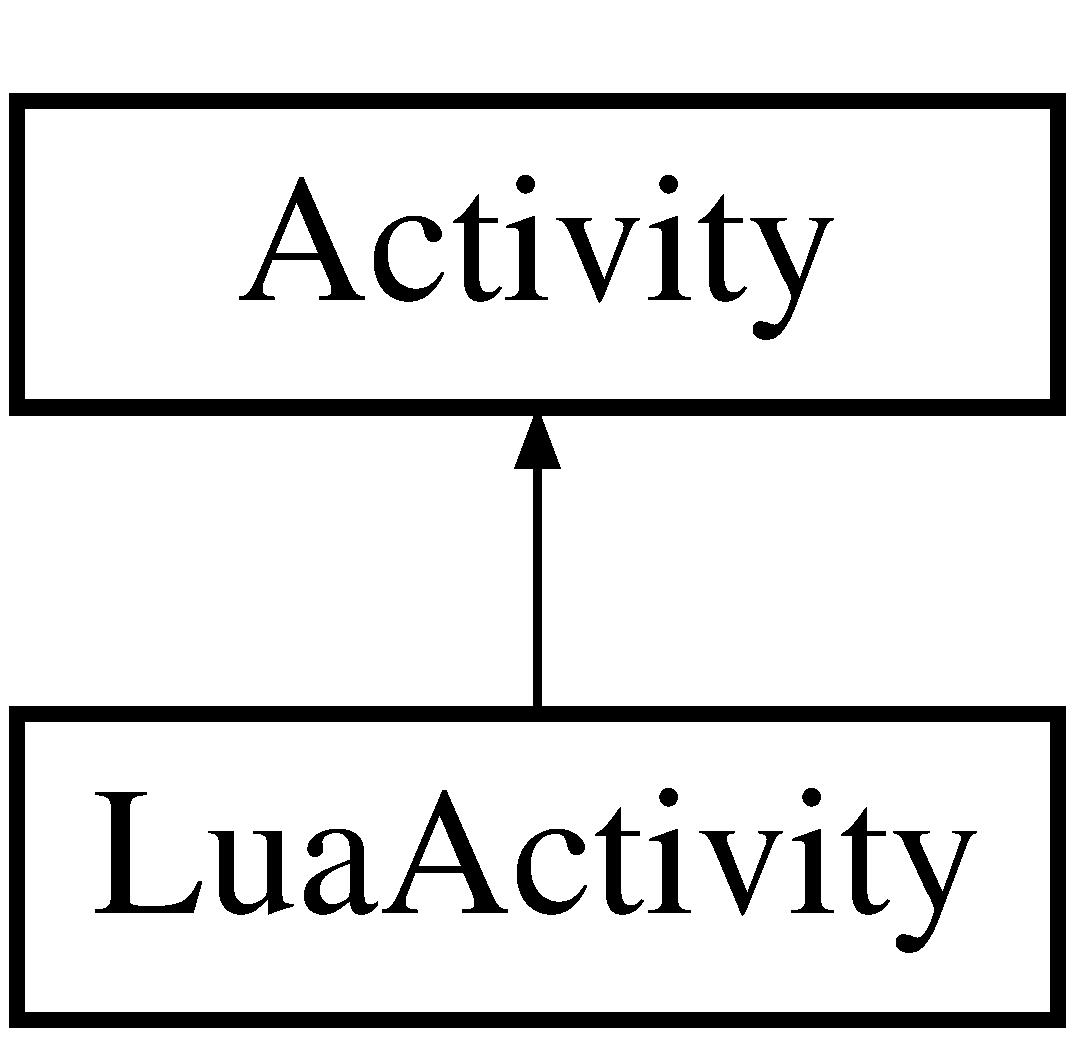
\includegraphics[height=2.000000cm]{classLuaActivity}
\end{center}
\end{figure}
\subsection*{Public Member Functions}
\begin{DoxyCompactItemize}
\item 
\hypertarget{classLuaActivity_a8eb438c54bfa69d3358539eab4838182}{{\bfseries Lua\-Activity} (std\-::string filename, std\-::string table)}\label{classLuaActivity_a8eb438c54bfa69d3358539eab4838182}

\item 
\hypertarget{classLuaActivity_a389d57bbec086396da7bebace6230e41}{void {\bfseries update} ()}\label{classLuaActivity_a389d57bbec086396da7bebace6230e41}

\item 
\hypertarget{classLuaActivity_ab2faeeaf6822a3b5ed02ef50e9568b53}{void {\bfseries render} ()}\label{classLuaActivity_ab2faeeaf6822a3b5ed02ef50e9568b53}

\end{DoxyCompactItemize}
\subsection*{Additional Inherited Members}


The documentation for this class was generated from the following files\-:\begin{DoxyCompactItemize}
\item 
/home/quentin/\-Projects/\-Asylia/include/activities/Lua\-Activity.\-hpp\item 
/home/quentin/\-Projects/\-Asylia/source/activities/Lua\-Activity.\-cpp\end{DoxyCompactItemize}

\hypertarget{classMap}{\section{Map Class Reference}
\label{classMap}\index{Map@{Map}}
}
\subsection*{Public Member Functions}
\begin{DoxyCompactItemize}
\item 
\hypertarget{classMap_a6bfec37d904bae26aa1a49d528389121}{{\bfseries Map} (const char $\ast$filename, u16 x, u16 y, u16 area, u8 layers, u16 tileset\-I\-D)}\label{classMap_a6bfec37d904bae26aa1a49d528389121}

\item 
\hypertarget{classMap_a00f29ed598774748bd9bf9f15b83d082}{void {\bfseries add\-Event} (\hyperlink{classEvent}{Event} $\ast$event)}\label{classMap_a00f29ed598774748bd9bf9f15b83d082}

\item 
\hypertarget{classMap_a69acc89957368e48c787a40f57fdb8ab}{\hyperlink{classEvent}{Event} $\ast$ {\bfseries get\-Event} (std\-::string name)}\label{classMap_a69acc89957368e48c787a40f57fdb8ab}

\item 
\hypertarget{classMap_a4ade1cf1f93b3de60ffdda3d9aa94bfa}{void {\bfseries events\-Update} ()}\label{classMap_a4ade1cf1f93b3de60ffdda3d9aa94bfa}

\item 
\hypertarget{classMap_a76acda70e2e2ff4392afa92afaa1cc06}{void {\bfseries update\-Events\-Actions} ()}\label{classMap_a76acda70e2e2ff4392afa92afaa1cc06}

\item 
\hypertarget{classMap_acc6cc4b358540c463100efad99a85ddd}{void {\bfseries load\-Tile} (u16 tile\-X, u16 tile\-Y, u8 layer)}\label{classMap_acc6cc4b358540c463100efad99a85ddd}

\item 
\hypertarget{classMap_a11fd1b88b5f3c923dad2c88df16e4373}{void {\bfseries load} ()}\label{classMap_a11fd1b88b5f3c923dad2c88df16e4373}

\item 
\hypertarget{classMap_a3be698445324a0d0e18b49d0730b9bea}{void {\bfseries render} ()}\label{classMap_a3be698445324a0d0e18b49d0730b9bea}

\item 
\hypertarget{classMap_adae49f3de52f3e48771b490ab929149a}{void {\bfseries render\-Overlay} ()}\label{classMap_adae49f3de52f3e48771b490ab929149a}

\item 
\hypertarget{classMap_a69a3d15b2e2223f7769ea4cab96cf9a7}{s16 {\bfseries get\-Tile} (u16 tile\-X, u16 tile\-Y, u16 layer)}\label{classMap_a69a3d15b2e2223f7769ea4cab96cf9a7}

\item 
\hypertarget{classMap_a18f14d389c84ca7d8f75a0a31fdf35f7}{\hyperlink{structTileset}{Tileset} $\ast$ {\bfseries tileset} () const }\label{classMap_a18f14d389c84ca7d8f75a0a31fdf35f7}

\item 
\hypertarget{classMap_aacc053785e87444e9232f7684686cb8f}{u16 {\bfseries width} () const }\label{classMap_aacc053785e87444e9232f7684686cb8f}

\item 
\hypertarget{classMap_a98253eaaf510d7de3f93c24c4dad96e3}{u16 {\bfseries height} () const }\label{classMap_a98253eaaf510d7de3f93c24c4dad96e3}

\item 
\hypertarget{classMap_adb7a36450acd05a790c04b70c13474ee}{u8 {\bfseries layers} () const }\label{classMap_adb7a36450acd05a790c04b70c13474ee}

\item 
\hypertarget{classMap_a40596b9dde8ddb9695b2e5bdc52417b4}{std\-::vector$<$ \hyperlink{classEvent}{Event} $\ast$ $>$ {\bfseries events} () const }\label{classMap_a40596b9dde8ddb9695b2e5bdc52417b4}

\item 
\hypertarget{classMap_ae26f0592f4a8f5503801afe4362db6c9}{\hyperlink{classImage}{Image} $\ast$ {\bfseries battleback} () const }\label{classMap_ae26f0592f4a8f5503801afe4362db6c9}

\item 
\hypertarget{classMap_ada9f5917144006f3f732435aefd2aa83}{void {\bfseries set\-Battleback} (\hyperlink{classImage}{Image} $\ast$battleback)}\label{classMap_ada9f5917144006f3f732435aefd2aa83}

\end{DoxyCompactItemize}
\subsection*{Static Public Member Functions}
\begin{DoxyCompactItemize}
\item 
\hypertarget{classMap_a2f4ff64ef6f3ed89e317ec975b4fdc10}{static s32 {\bfseries get\-Scroll\-X} ()}\label{classMap_a2f4ff64ef6f3ed89e317ec975b4fdc10}

\item 
\hypertarget{classMap_acbb4890c88051aa441ad7f5211aa63a4}{static s32 {\bfseries get\-Scroll\-Y} ()}\label{classMap_acbb4890c88051aa441ad7f5211aa63a4}

\item 
\hypertarget{classMap_a62675cd66f25e784a7abd6e40ec2dee7}{static void {\bfseries center\-Map\-With\-Object} (s16 x, s16 y, u16 w, u16 h)}\label{classMap_a62675cd66f25e784a7abd6e40ec2dee7}

\end{DoxyCompactItemize}
\subsection*{Static Public Attributes}
\begin{DoxyCompactItemize}
\item 
\hypertarget{classMap_ac7681948af9e655b44605fcccc0217ed}{static s32 {\bfseries scroll\-X} = 0}\label{classMap_ac7681948af9e655b44605fcccc0217ed}

\item 
\hypertarget{classMap_a55e0dcce25c5008a4c80ff9f509d87d4}{static s32 {\bfseries scroll\-Y} = 0}\label{classMap_a55e0dcce25c5008a4c80ff9f509d87d4}

\end{DoxyCompactItemize}


The documentation for this class was generated from the following files\-:\begin{DoxyCompactItemize}
\item 
/home/quentin/\-Projects/\-Asylia/include/display/Map.\-hpp\item 
/home/quentin/\-Projects/\-Asylia/source/display/Map.\-cpp\end{DoxyCompactItemize}

\hypertarget{classMapActivity}{\section{Map\-Activity Class Reference}
\label{classMapActivity}\index{Map\-Activity@{Map\-Activity}}
}
Inheritance diagram for Map\-Activity\-:\begin{figure}[H]
\begin{center}
\leavevmode
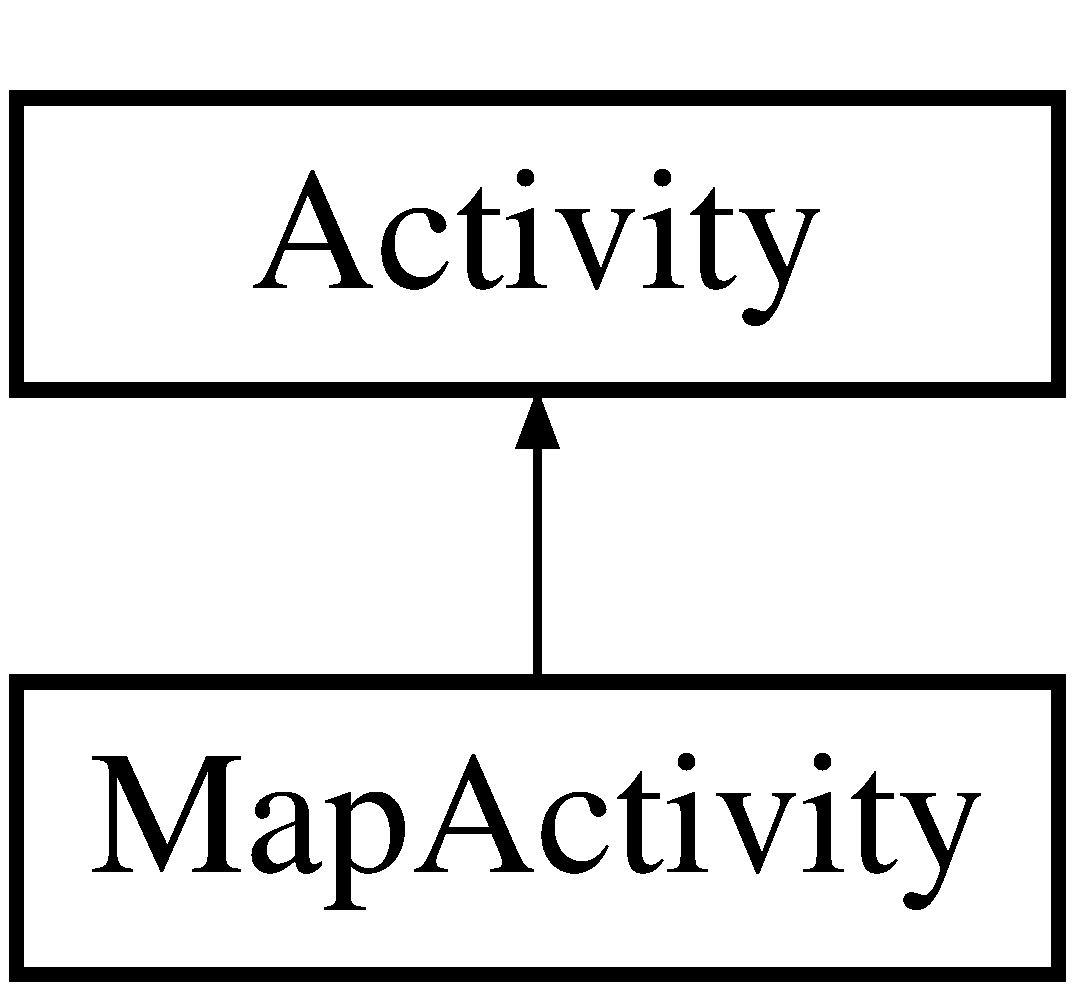
\includegraphics[height=2.000000cm]{classMapActivity}
\end{center}
\end{figure}
\subsection*{Public Member Functions}
\begin{DoxyCompactItemize}
\item 
\hypertarget{classMapActivity_a76aef9e9aefd80668becf9dc93345ba9}{void {\bfseries init} ()}\label{classMapActivity_a76aef9e9aefd80668becf9dc93345ba9}

\item 
\hypertarget{classMapActivity_aca3e8d6ee07c7e8a16cb64ae14d9e256}{void {\bfseries update} ()}\label{classMapActivity_aca3e8d6ee07c7e8a16cb64ae14d9e256}

\item 
\hypertarget{classMapActivity_a1b90f9cd60a8bf01047397fcc2b1a5c9}{void {\bfseries render} ()}\label{classMapActivity_a1b90f9cd60a8bf01047397fcc2b1a5c9}

\end{DoxyCompactItemize}
\subsection*{Additional Inherited Members}


The documentation for this class was generated from the following files\-:\begin{DoxyCompactItemize}
\item 
/home/quentin/\-Projects/\-Asylia/include/activities/Map\-Activity.\-hpp\item 
/home/quentin/\-Projects/\-Asylia/source/activities/Map\-Activity.\-cpp\end{DoxyCompactItemize}

\hypertarget{classMapManager}{\section{Map\-Manager Class Reference}
\label{classMapManager}\index{Map\-Manager@{Map\-Manager}}
}
\subsection*{Static Public Member Functions}
\begin{DoxyCompactItemize}
\item 
\hypertarget{classMapManager_abac61fe753811dabe315396d1410537a}{static void {\bfseries init} ()}\label{classMapManager_abac61fe753811dabe315396d1410537a}

\item 
\hypertarget{classMapManager_a69f9992c032468fc5420a11aa5dfa737}{static void {\bfseries free} ()}\label{classMapManager_a69f9992c032468fc5420a11aa5dfa737}

\item 
\hypertarget{classMapManager_aab0844b3d4e9b1d1c70932541bd9120d}{static void {\bfseries init\-Tilesets} ()}\label{classMapManager_aab0844b3d4e9b1d1c70932541bd9120d}

\item 
\hypertarget{classMapManager_ae211956a705522b9c105a619731e8ad7}{static void {\bfseries init\-Maps} ()}\label{classMapManager_ae211956a705522b9c105a619731e8ad7}

\end{DoxyCompactItemize}
\subsection*{Static Public Attributes}
\begin{DoxyCompactItemize}
\item 
\hypertarget{classMapManager_a13d7a8755a733da69075bbefb67d287b}{static std\-::vector$<$ \hyperlink{structTileset}{Tileset} $\ast$ $>$ {\bfseries tilesets}}\label{classMapManager_a13d7a8755a733da69075bbefb67d287b}

\item 
\hypertarget{classMapManager_a640acf692080c83621a463ce4604ae6c}{static std\-::vector\\*
$<$ std\-::vector$<$ \hyperlink{classMap}{Map} $\ast$ $>$ $>$ {\bfseries maps}}\label{classMapManager_a640acf692080c83621a463ce4604ae6c}

\item 
\hypertarget{classMapManager_abb96d305c1da367d2decd56ea2796913}{static \hyperlink{classMap}{Map} $\ast$ {\bfseries current\-Map} = N\-U\-L\-L}\label{classMapManager_abb96d305c1da367d2decd56ea2796913}

\end{DoxyCompactItemize}


The documentation for this class was generated from the following files\-:\begin{DoxyCompactItemize}
\item 
/home/quentin/\-Projects/\-Asylia/include/managers/Map\-Manager.\-hpp\item 
/home/quentin/\-Projects/\-Asylia/source/display/Map\-Manager.\-cpp\end{DoxyCompactItemize}

\hypertarget{classMenuActivity}{\section{Menu\-Activity Class Reference}
\label{classMenuActivity}\index{Menu\-Activity@{Menu\-Activity}}
}
Inheritance diagram for Menu\-Activity\-:\begin{figure}[H]
\begin{center}
\leavevmode
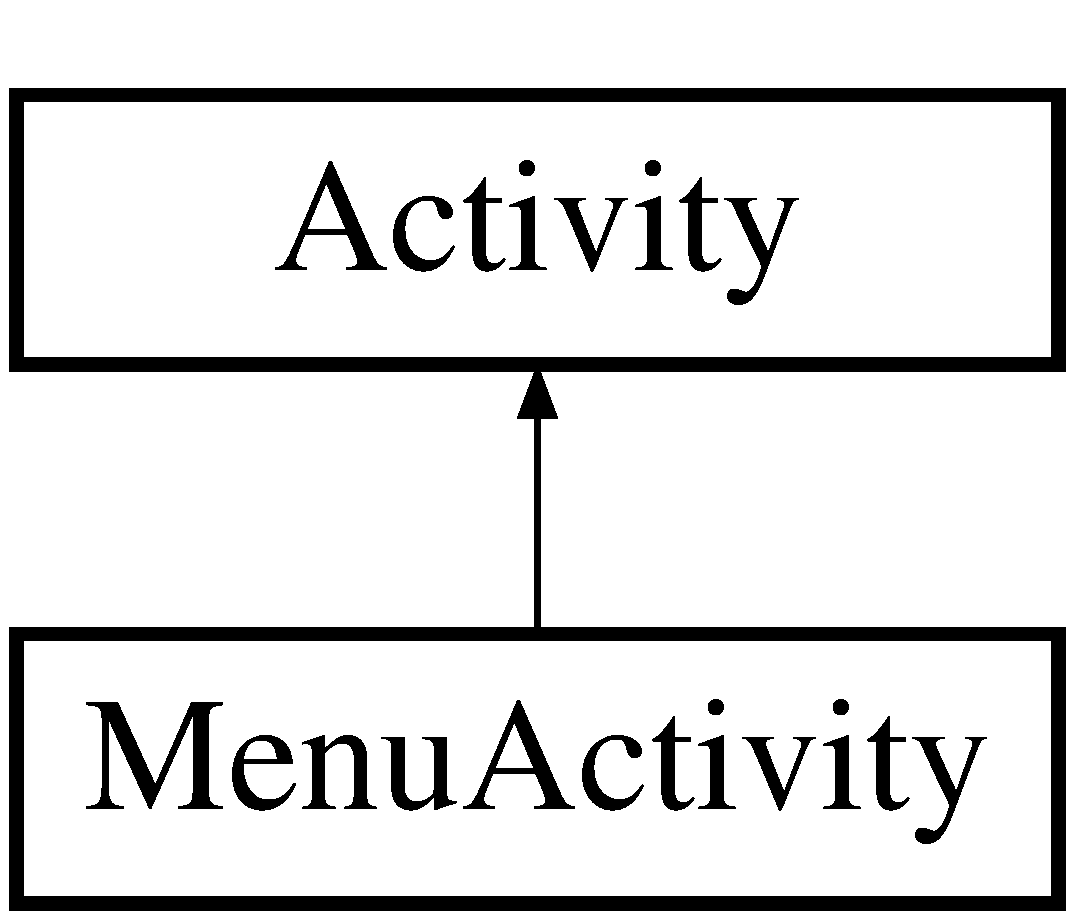
\includegraphics[height=2.000000cm]{classMenuActivity}
\end{center}
\end{figure}
\subsection*{Public Member Functions}
\begin{DoxyCompactItemize}
\item 
\hypertarget{classMenuActivity_a1d4c791e5b9b3eedb57eaa9dd7a794ad}{{\bfseries Menu\-Activity} (\hyperlink{classActivity}{Activity} $\ast$parent=N\-U\-L\-L)}\label{classMenuActivity_a1d4c791e5b9b3eedb57eaa9dd7a794ad}

\item 
\hypertarget{classMenuActivity_a06ee325cd062a218cc5385dae31dcb8c}{void {\bfseries load\-Command\-Window} ()}\label{classMenuActivity_a06ee325cd062a218cc5385dae31dcb8c}

\item 
\hypertarget{classMenuActivity_a2c3d27f669bc15084a965878dfe32181}{void {\bfseries update} ()}\label{classMenuActivity_a2c3d27f669bc15084a965878dfe32181}

\item 
\hypertarget{classMenuActivity_a1e4de0a5320d975b44ca5ad7745dc15b}{void {\bfseries render} ()}\label{classMenuActivity_a1e4de0a5320d975b44ca5ad7745dc15b}

\item 
\hypertarget{classMenuActivity_af5ffdd1998f117c64b23e7261b193768}{\hyperlink{classCommandWindow}{Command\-Window} $\ast$ {\bfseries cmdwin} ()}\label{classMenuActivity_af5ffdd1998f117c64b23e7261b193768}

\item 
\hypertarget{classMenuActivity_a58570dad2334ca37848b33217e10d2b8}{void {\bfseries actor\-Choice\-Mode\-On} ()}\label{classMenuActivity_a58570dad2334ca37848b33217e10d2b8}

\end{DoxyCompactItemize}
\subsection*{Additional Inherited Members}


The documentation for this class was generated from the following files\-:\begin{DoxyCompactItemize}
\item 
/home/quentin/\-Projects/\-Asylia/include/activities/Menu\-Activity.\-hpp\item 
/home/quentin/\-Projects/\-Asylia/source/activities/Menu\-Activity.\-cpp\end{DoxyCompactItemize}

\hypertarget{classMessageActivity}{\section{Message\-Activity Class Reference}
\label{classMessageActivity}\index{Message\-Activity@{Message\-Activity}}
}
Inheritance diagram for Message\-Activity\-:\begin{figure}[H]
\begin{center}
\leavevmode
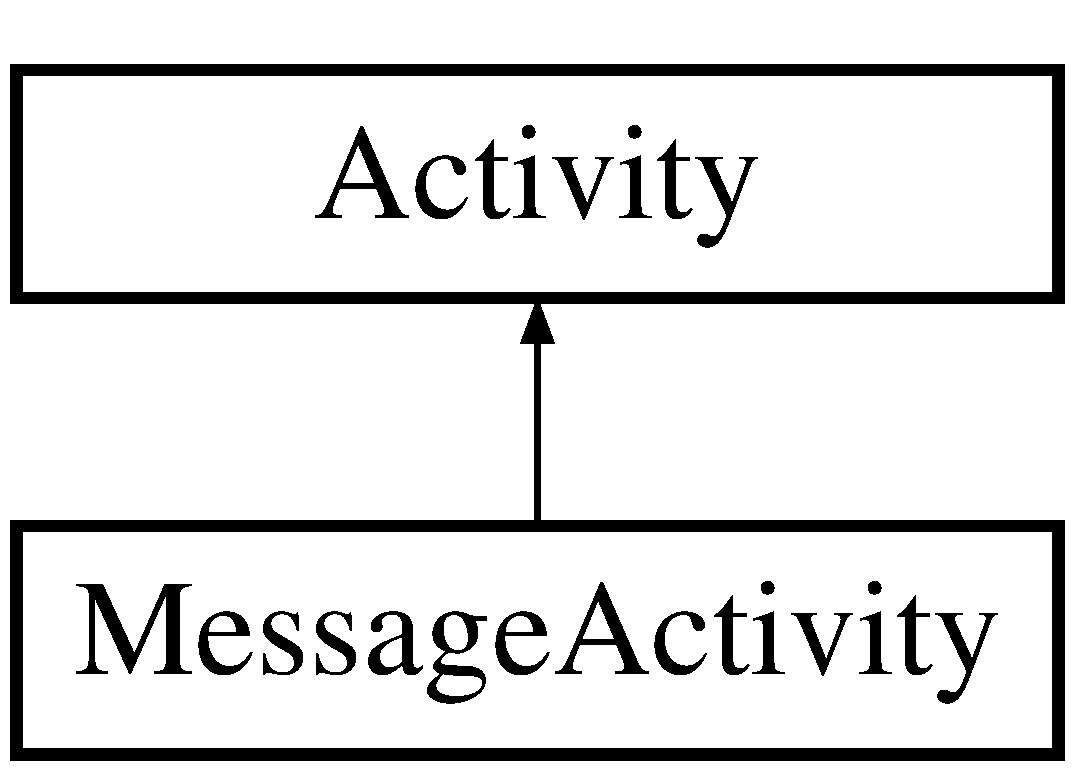
\includegraphics[height=2.000000cm]{classMessageActivity}
\end{center}
\end{figure}
\subsection*{Public Member Functions}
\begin{DoxyCompactItemize}
\item 
\hypertarget{classMessageActivity_aa9219936e76d953fb8dbf6337b168d75}{{\bfseries Message\-Activity} (std\-::string message, \hyperlink{classActivity}{Activity} $\ast$parent=N\-U\-L\-L)}\label{classMessageActivity_aa9219936e76d953fb8dbf6337b168d75}

\item 
\hypertarget{classMessageActivity_ab01b1d6eb0e0e53cdd8caaeadaab7468}{void {\bfseries add\-Command} (std\-::string command)}\label{classMessageActivity_ab01b1d6eb0e0e53cdd8caaeadaab7468}

\item 
\hypertarget{classMessageActivity_a657f22456b3902b757a85272b9fdd040}{void {\bfseries update\-Cmdwin\-Size} ()}\label{classMessageActivity_a657f22456b3902b757a85272b9fdd040}

\item 
\hypertarget{classMessageActivity_a1f5c5b3b669f1c22bbe38434e6bf37f3}{u16 {\bfseries get\-Cmdwin\-Pos} ()}\label{classMessageActivity_a1f5c5b3b669f1c22bbe38434e6bf37f3}

\item 
\hypertarget{classMessageActivity_a23c9d5373ce29e95643b3e35473297fb}{void {\bfseries update} ()}\label{classMessageActivity_a23c9d5373ce29e95643b3e35473297fb}

\item 
\hypertarget{classMessageActivity_ad2c57661dd561d6d0f833b08a25c6a76}{void {\bfseries render} ()}\label{classMessageActivity_ad2c57661dd561d6d0f833b08a25c6a76}

\end{DoxyCompactItemize}
\subsection*{Additional Inherited Members}


The documentation for this class was generated from the following files\-:\begin{DoxyCompactItemize}
\item 
/home/quentin/\-Projects/\-Asylia/include/activities/Message\-Activity.\-hpp\item 
/home/quentin/\-Projects/\-Asylia/source/activities/Message\-Activity.\-cpp\end{DoxyCompactItemize}

\hypertarget{classParameter}{\section{Parameter Class Reference}
\label{classParameter}\index{Parameter@{Parameter}}
}
Inheritance diagram for Parameter\-:\begin{figure}[H]
\begin{center}
\leavevmode
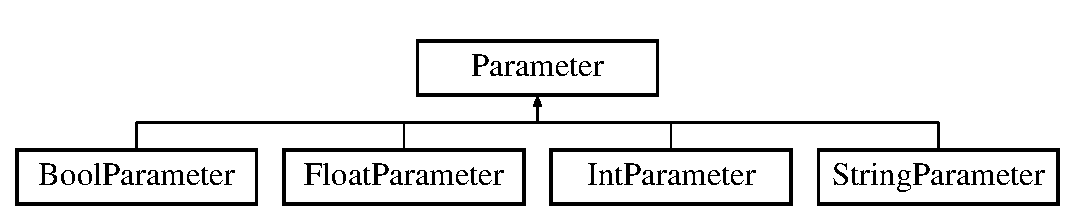
\includegraphics[height=2.000000cm]{classParameter}
\end{center}
\end{figure}
\subsection*{Public Types}
\begin{DoxyCompactItemize}
\item 
enum {\bfseries Type} \{ \\*
{\bfseries Undefined}, 
{\bfseries Int\-Parameter}, 
{\bfseries Bool\-Parameter}, 
{\bfseries Float\-Parameter}, 
\\*
{\bfseries String\-Parameter}
 \}
\end{DoxyCompactItemize}
\subsection*{Public Member Functions}
\begin{DoxyCompactItemize}
\item 
\hypertarget{classParameter_a7c153c936909b52f3fdbf2ba3b328dcb}{virtual void $\ast$ {\bfseries value} ()=0}\label{classParameter_a7c153c936909b52f3fdbf2ba3b328dcb}

\item 
\hypertarget{classParameter_ae70ff10b9fa2ab2458286c411a2cb5be}{bool {\bfseries is\-Integer} ()}\label{classParameter_ae70ff10b9fa2ab2458286c411a2cb5be}

\item 
\hypertarget{classParameter_a0c25100815bda4ae19801fc146529535}{bool {\bfseries is\-Boolean} ()}\label{classParameter_a0c25100815bda4ae19801fc146529535}

\item 
\hypertarget{classParameter_a98c8b305c1e1be9a02240233dac083d9}{bool {\bfseries is\-Float} ()}\label{classParameter_a98c8b305c1e1be9a02240233dac083d9}

\item 
\hypertarget{classParameter_a005bd9dc4f0520cfec7d4a87d7613287}{bool {\bfseries is\-String} ()}\label{classParameter_a005bd9dc4f0520cfec7d4a87d7613287}

\item 
\hypertarget{classParameter_af5a165fc9bcfa0d9b2abd0777cb433bd}{Type {\bfseries type} () const }\label{classParameter_af5a165fc9bcfa0d9b2abd0777cb433bd}

\end{DoxyCompactItemize}
\subsection*{Protected Attributes}
\begin{DoxyCompactItemize}
\item 
\hypertarget{classParameter_a088830b8d164206cface0a89af79f108}{Type {\bfseries m\-\_\-type}}\label{classParameter_a088830b8d164206cface0a89af79f108}

\end{DoxyCompactItemize}


The documentation for this class was generated from the following files\-:\begin{DoxyCompactItemize}
\item 
/home/quentin/\-Projects/\-Asylia/include/core/Parameter.\-hpp\item 
/home/quentin/\-Projects/\-Asylia/source/core/Parameter.\-cpp\end{DoxyCompactItemize}

\hypertarget{classParameterList}{\section{Parameter\-List Class Reference}
\label{classParameterList}\index{Parameter\-List@{Parameter\-List}}
}
\subsection*{Public Member Functions}
\begin{DoxyCompactItemize}
\item 
\hypertarget{classParameterList_acaad445445e1d62203322e3f5c049172}{{\bfseries Parameter\-List} (const \hyperlink{classParameterList}{Parameter\-List} \&list)}\label{classParameterList_acaad445445e1d62203322e3f5c049172}

\item 
\hypertarget{classParameterList_a6f2125f1182f2615d5b4e4ce5351651f}{void {\bfseries clear} ()}\label{classParameterList_a6f2125f1182f2615d5b4e4ce5351651f}

\item 
\hypertarget{classParameterList_a5337ced79cbaf86cda826f99f3c622fa}{\hyperlink{classParameter}{Parameter} $\ast$ {\bfseries at} (u16 id) const }\label{classParameterList_a5337ced79cbaf86cda826f99f3c622fa}

\item 
\hypertarget{classParameterList_af413109556e5e36b89bbd9e63e64fb54}{\hyperlink{classParameter}{Parameter} $\ast$ {\bfseries operator\mbox{[}$\,$\mbox{]}} (u16 id) const }\label{classParameterList_af413109556e5e36b89bbd9e63e64fb54}

\item 
\hypertarget{classParameterList_a398b37da9adf25660d5646cb52fb94e1}{u16 {\bfseries size} () const }\label{classParameterList_a398b37da9adf25660d5646cb52fb94e1}

\item 
\hypertarget{classParameterList_a63f35d0e0e11936de0e13ef3246b1fef}{void {\bfseries add\-Int\-Parameter} (int param)}\label{classParameterList_a63f35d0e0e11936de0e13ef3246b1fef}

\item 
\hypertarget{classParameterList_a2ccd2e18b60b3f2789779031d62e41b3}{void {\bfseries add\-Bool\-Parameter} (bool param)}\label{classParameterList_a2ccd2e18b60b3f2789779031d62e41b3}

\item 
\hypertarget{classParameterList_a3be261ee73ebea19edb18bd233994af1}{void {\bfseries add\-Float\-Parameter} (float param)}\label{classParameterList_a3be261ee73ebea19edb18bd233994af1}

\item 
\hypertarget{classParameterList_ab7f3c8ec0b1d4ee4e614c3fdd588a245}{void {\bfseries add\-String\-Parameter} (std\-::string param)}\label{classParameterList_ab7f3c8ec0b1d4ee4e614c3fdd588a245}

\end{DoxyCompactItemize}


The documentation for this class was generated from the following files\-:\begin{DoxyCompactItemize}
\item 
/home/quentin/\-Projects/\-Asylia/include/core/Parameter.\-hpp\item 
/home/quentin/\-Projects/\-Asylia/source/core/Parameter.\-cpp\end{DoxyCompactItemize}

\hypertarget{classPlayer}{\section{Player Class Reference}
\label{classPlayer}\index{Player@{Player}}
}
Inheritance diagram for Player\-:\begin{figure}[H]
\begin{center}
\leavevmode
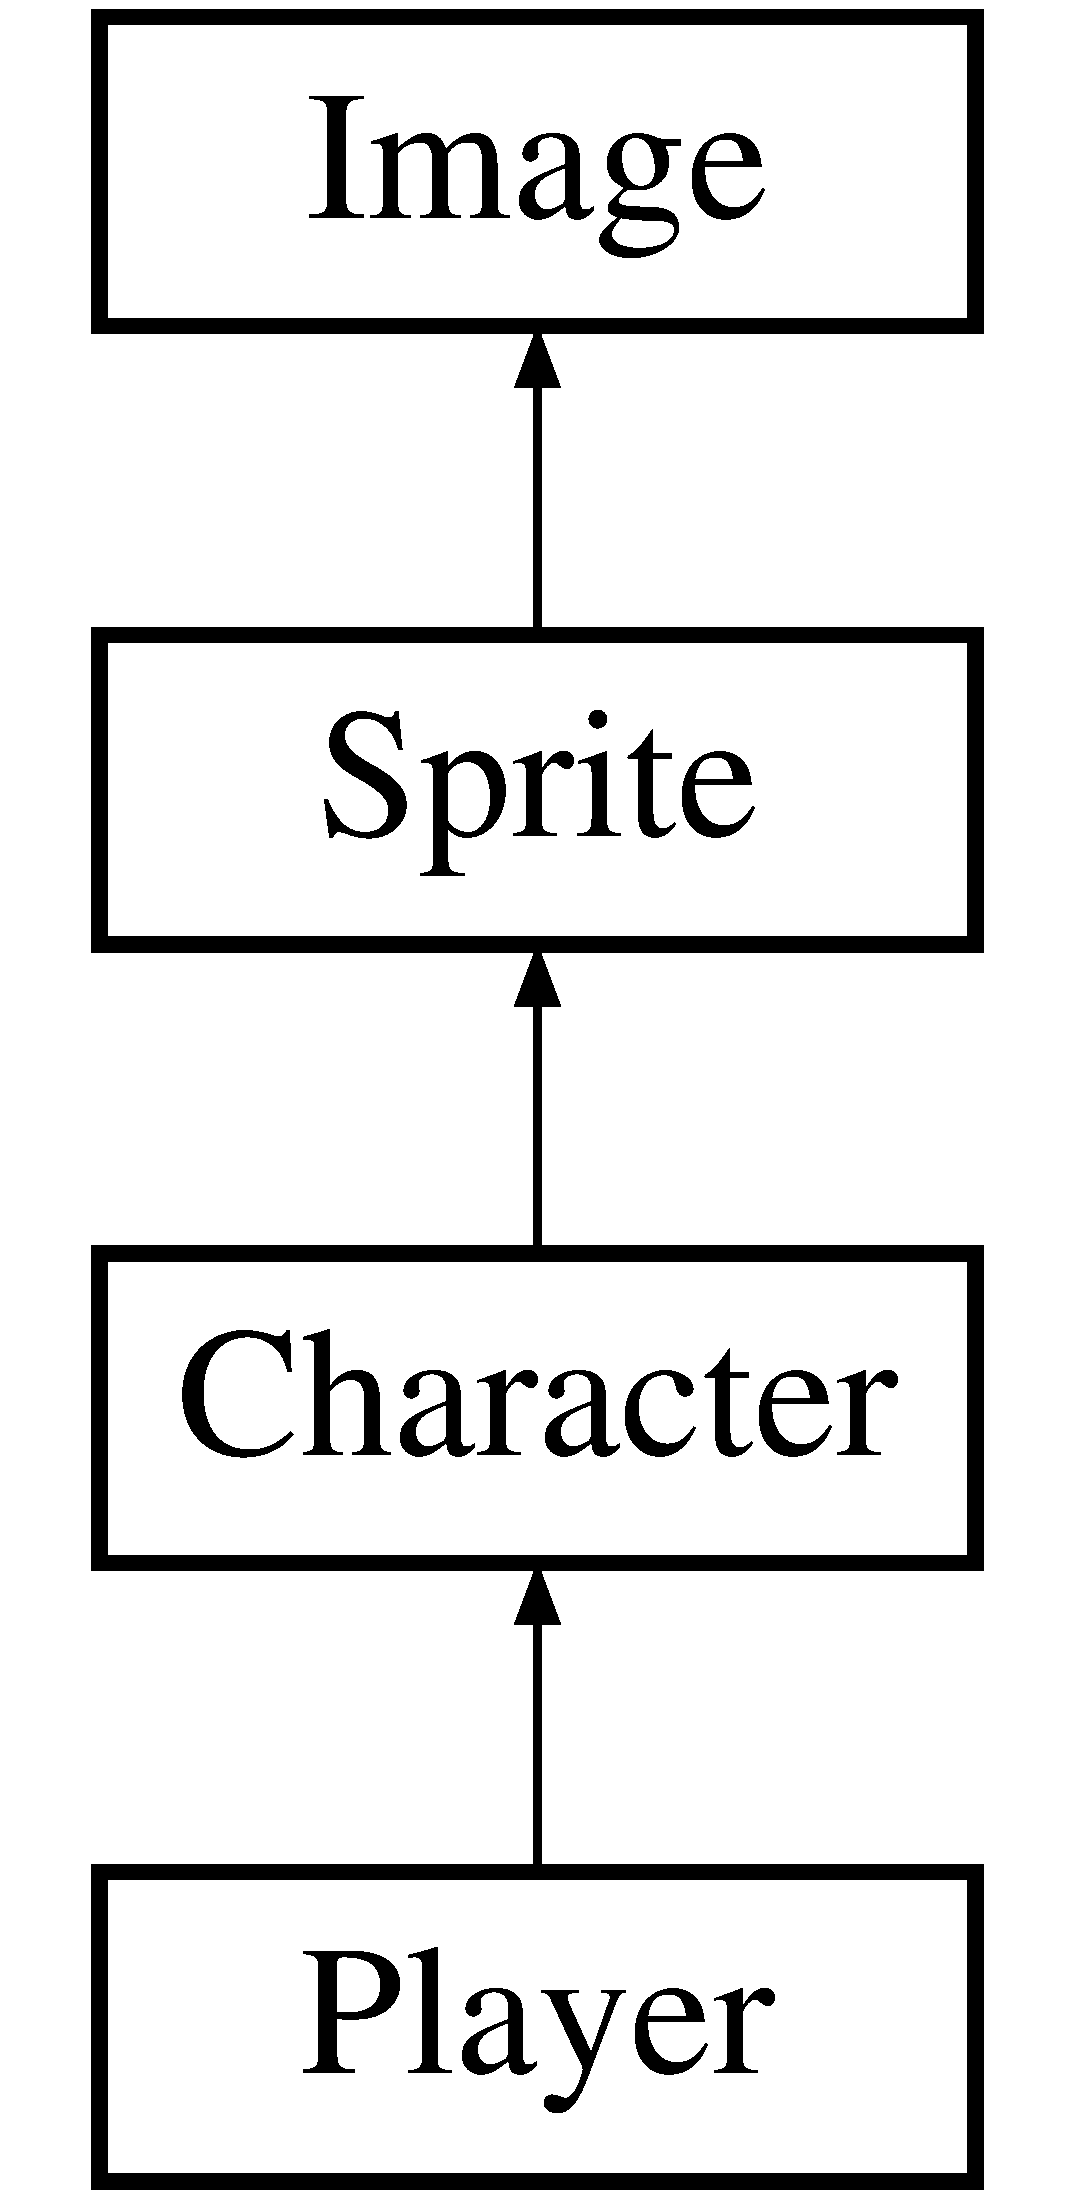
\includegraphics[height=4.000000cm]{classPlayer}
\end{center}
\end{figure}
\subsection*{Public Member Functions}
\begin{DoxyCompactItemize}
\item 
\hypertarget{classPlayer_a36ce5c199bdbb064ae6c366aa809667d}{{\bfseries Player} (std\-::string filename, s16 x, s16 y, u8 direction)}\label{classPlayer_a36ce5c199bdbb064ae6c366aa809667d}

\item 
\hypertarget{classPlayer_ae02ee46d8c20dd0697b975f935b09839}{void {\bfseries move} ()}\label{classPlayer_ae02ee46d8c20dd0697b975f935b09839}

\item 
\hypertarget{classPlayer_a87cf2ed24622b893c95fafc0fe7b690b}{void {\bfseries add\-Team\-Member} (u16 id)}\label{classPlayer_a87cf2ed24622b893c95fafc0fe7b690b}

\item 
\hypertarget{classPlayer_af0c2183a1d68d82104065a8e1671437c}{\hyperlink{classActor}{Actor} $\ast$ {\bfseries get\-Team\-Member} (u8 i)}\label{classPlayer_af0c2183a1d68d82104065a8e1671437c}

\item 
\hypertarget{classPlayer_aa0b58cbbe1676b94136381a8a10131c1}{u16 {\bfseries team\-Size} ()}\label{classPlayer_aa0b58cbbe1676b94136381a8a10131c1}

\end{DoxyCompactItemize}
\subsection*{Additional Inherited Members}


The documentation for this class was generated from the following files\-:\begin{DoxyCompactItemize}
\item 
/home/quentin/\-Projects/\-Asylia/include/entities/Player.\-hpp\item 
/home/quentin/\-Projects/\-Asylia/source/entities/Player.\-cpp\end{DoxyCompactItemize}

\hypertarget{classQuest}{\section{Quest Class Reference}
\label{classQuest}\index{Quest@{Quest}}
}
\subsection*{Public Member Functions}
\begin{DoxyCompactItemize}
\item 
\hypertarget{classQuest_a466310544e301430508002377e8c6d89}{{\bfseries Quest} (u16 exp, u16 gold)}\label{classQuest_a466310544e301430508002377e8c6d89}

\item 
\hypertarget{classQuest_a5f1e4f26812517bf218e290dec85accb}{void {\bfseries add\-Objective} (\hyperlink{classQuestObjective}{Quest\-Objective} $\ast$objective)}\label{classQuest_a5f1e4f26812517bf218e290dec85accb}

\item 
\hypertarget{classQuest_a571cae81f911bbb9944d334a636b0559}{\hyperlink{classInventory}{Inventory} $\ast$ {\bfseries items} ()}\label{classQuest_a571cae81f911bbb9944d334a636b0559}

\end{DoxyCompactItemize}
\subsection*{Static Public Attributes}
\begin{DoxyCompactItemize}
\item 
\hypertarget{classQuest_a6515264d74da1bbe92f4cc22b7bc679b}{static u16 {\bfseries counter} = 0}\label{classQuest_a6515264d74da1bbe92f4cc22b7bc679b}

\end{DoxyCompactItemize}


The documentation for this class was generated from the following files\-:\begin{DoxyCompactItemize}
\item 
/home/quentin/\-Projects/\-Asylia/include/quests/Quest.\-hpp\item 
/home/quentin/\-Projects/\-Asylia/source/quests/Quest.\-cpp\end{DoxyCompactItemize}

\hypertarget{classQuestObjective}{\section{Quest\-Objective Class Reference}
\label{classQuestObjective}\index{Quest\-Objective@{Quest\-Objective}}
}
\subsection*{Public Types}
\begin{DoxyCompactItemize}
\item 
enum {\bfseries Type} \{ \\*
{\bfseries Undefined}, 
{\bfseries Bring\-Item}, 
{\bfseries Get\-Item}, 
{\bfseries Beat\-Enemy}, 
\\*
{\bfseries Talk\-To\-Someone}
 \}
\end{DoxyCompactItemize}
\subsection*{Public Member Functions}
\begin{DoxyCompactItemize}
\item 
\hypertarget{classQuestObjective_a0608ed6e0fb3b82f670bedf4f1da32fc}{{\bfseries Quest\-Objective} (u16 item\-To\-Bring, Item\-::\-Type type)}\label{classQuestObjective_a0608ed6e0fb3b82f670bedf4f1da32fc}

\item 
\hypertarget{classQuestObjective_ad197a9e364a07e5388a4a48743633d6c}{{\bfseries Quest\-Objective} (u16 item\-To\-Get, Item\-::\-Type type, u16 count)}\label{classQuestObjective_ad197a9e364a07e5388a4a48743633d6c}

\item 
\hypertarget{classQuestObjective_a19542be0be15f37918ba27a232715eb5}{{\bfseries Quest\-Objective} (u16 enemy\-To\-Beat, u16 count)}\label{classQuestObjective_a19542be0be15f37918ba27a232715eb5}

\item 
\hypertarget{classQuestObjective_a5207c9132c4dd43e03829ea1ca2c76c7}{{\bfseries Quest\-Objective} (std\-::string event\-To\-Talk\-To)}\label{classQuestObjective_a5207c9132c4dd43e03829ea1ca2c76c7}

\end{DoxyCompactItemize}
\subsection*{Protected Attributes}
\begin{DoxyCompactItemize}
\item 
\hypertarget{classQuestObjective_a14066d424437ebce3cc48a9de012701e}{Type {\bfseries m\-\_\-type}}\label{classQuestObjective_a14066d424437ebce3cc48a9de012701e}

\item 
\hypertarget{classQuestObjective_a3a05cce8bb2766698e687f0c77380a83}{\hyperlink{classParameterList}{Parameter\-List} {\bfseries m\-\_\-params}}\label{classQuestObjective_a3a05cce8bb2766698e687f0c77380a83}

\end{DoxyCompactItemize}


The documentation for this class was generated from the following file\-:\begin{DoxyCompactItemize}
\item 
/home/quentin/\-Projects/\-Asylia/include/quests/Quest\-Objective.\-hpp\end{DoxyCompactItemize}

\hypertarget{structRectangle}{\section{Rectangle Struct Reference}
\label{structRectangle}\index{Rectangle@{Rectangle}}
}
\subsection*{Public Member Functions}
\begin{DoxyCompactItemize}
\item 
\hypertarget{structRectangle_a602bf07738bc080fcc4014232d5a52b5}{{\bfseries Rectangle} (s16 \-\_\-x, s16 \-\_\-y, u16 \-\_\-width, u16 \-\_\-height)}\label{structRectangle_a602bf07738bc080fcc4014232d5a52b5}

\end{DoxyCompactItemize}
\subsection*{Public Attributes}
\begin{DoxyCompactItemize}
\item 
\hypertarget{structRectangle_acfdfea445db55a8783bfce265bccd77c}{s16 {\bfseries x}}\label{structRectangle_acfdfea445db55a8783bfce265bccd77c}

\item 
\hypertarget{structRectangle_a04785954856a12078847ffda7ff52ec3}{s16 {\bfseries y}}\label{structRectangle_a04785954856a12078847ffda7ff52ec3}

\item 
\hypertarget{structRectangle_acb97cf4251b89c0e8fc5a749827f267a}{u16 {\bfseries width}}\label{structRectangle_acb97cf4251b89c0e8fc5a749827f267a}

\item 
\hypertarget{structRectangle_ace4a1f5cf716f05c1d6e42299c759d19}{u16 {\bfseries height}}\label{structRectangle_ace4a1f5cf716f05c1d6e42299c759d19}

\end{DoxyCompactItemize}


The documentation for this struct was generated from the following file\-:\begin{DoxyCompactItemize}
\item 
/home/quentin/\-Projects/\-Asylia/include/core/Rectangle.\-hpp\end{DoxyCompactItemize}

\hypertarget{classSelectableWindow}{\section{Selectable\-Window Class Reference}
\label{classSelectableWindow}\index{Selectable\-Window@{Selectable\-Window}}
}
Inheritance diagram for Selectable\-Window\-:\begin{figure}[H]
\begin{center}
\leavevmode
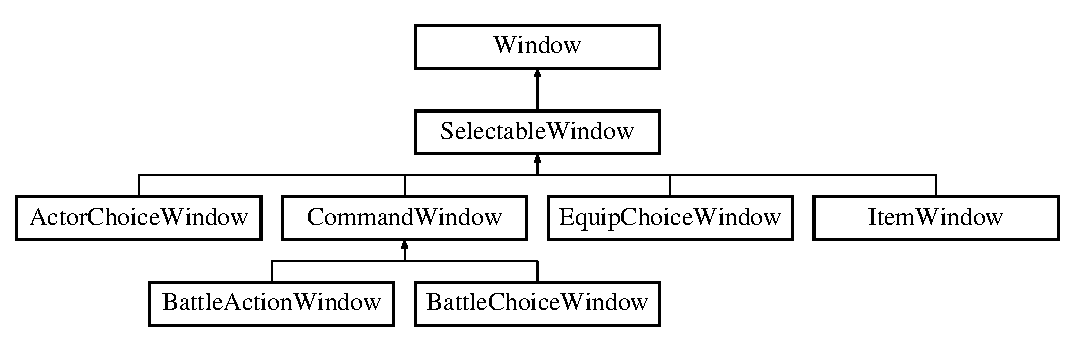
\includegraphics[height=4.000000cm]{classSelectableWindow}
\end{center}
\end{figure}
\subsection*{Public Member Functions}
\begin{DoxyCompactItemize}
\item 
\hypertarget{classSelectableWindow_abdf0b9056eb66248ecf1020a0a668b5f}{{\bfseries Selectable\-Window} (s16 x, s16 y, u16 width, u16 height)}\label{classSelectableWindow_abdf0b9056eb66248ecf1020a0a668b5f}

\item 
\hypertarget{classSelectableWindow_ae9fad1c1c7208df039e8b9fa5e7374b2}{void {\bfseries update\-Cursor} ()}\label{classSelectableWindow_ae9fad1c1c7208df039e8b9fa5e7374b2}

\item 
\hypertarget{classSelectableWindow_aa881020eda312ed8f11b1fd11cfe8a26}{void {\bfseries update} ()}\label{classSelectableWindow_aa881020eda312ed8f11b1fd11cfe8a26}

\item 
\hypertarget{classSelectableWindow_a039c71387c608d0704d65001e6a6836e}{u16 {\bfseries item\-Max} () const }\label{classSelectableWindow_a039c71387c608d0704d65001e6a6836e}

\item 
\hypertarget{classSelectableWindow_a75ffe4a1e88d35abddc3b68a831dbe91}{s16 {\bfseries pos} () const }\label{classSelectableWindow_a75ffe4a1e88d35abddc3b68a831dbe91}

\item 
\hypertarget{classSelectableWindow_ab3645b68efa7d6b18863e0bdada9c78f}{void {\bfseries pos} (u16 pos)}\label{classSelectableWindow_ab3645b68efa7d6b18863e0bdada9c78f}

\end{DoxyCompactItemize}
\subsection*{Static Public Attributes}
\begin{DoxyCompactItemize}
\item 
\hypertarget{classSelectableWindow_a148a4bf43c59ad0af9e7d95a9ec6e2ae}{static u16 {\bfseries last\-Pos} = 0}\label{classSelectableWindow_a148a4bf43c59ad0af9e7d95a9ec6e2ae}

\end{DoxyCompactItemize}
\subsection*{Protected Attributes}
\begin{DoxyCompactItemize}
\item 
\hypertarget{classSelectableWindow_a47b0055334e7ca5c11e8f9945dccdd2d}{u16 {\bfseries m\-\_\-item\-Max}}\label{classSelectableWindow_a47b0055334e7ca5c11e8f9945dccdd2d}

\item 
\hypertarget{classSelectableWindow_adc7dd0ae783888cef0b79cb213e330d4}{u8 {\bfseries m\-\_\-column\-Max}}\label{classSelectableWindow_adc7dd0ae783888cef0b79cb213e330d4}

\item 
\hypertarget{classSelectableWindow_a4cede24d2226f928b29dcb0c32b3aa30}{s16 {\bfseries m\-\_\-pos}}\label{classSelectableWindow_a4cede24d2226f928b29dcb0c32b3aa30}

\item 
\hypertarget{classSelectableWindow_a949a88001a4c8d48306a59728966411e}{u8 {\bfseries m\-\_\-scroll}}\label{classSelectableWindow_a949a88001a4c8d48306a59728966411e}

\item 
\hypertarget{classSelectableWindow_af50ebd7a84ac520fa2b9909c94ac2397}{\hyperlink{classInfoWindow}{Info\-Window} $\ast$ {\bfseries m\-\_\-info\-Window}}\label{classSelectableWindow_af50ebd7a84ac520fa2b9909c94ac2397}

\end{DoxyCompactItemize}


The documentation for this class was generated from the following files\-:\begin{DoxyCompactItemize}
\item 
/home/quentin/\-Projects/\-Asylia/include/windows/Selectable\-Window.\-hpp\item 
/home/quentin/\-Projects/\-Asylia/source/windows/Selectable\-Window.\-cpp\end{DoxyCompactItemize}

\hypertarget{classSettingsActivity}{\section{Settings\-Activity Class Reference}
\label{classSettingsActivity}\index{Settings\-Activity@{Settings\-Activity}}
}
Inheritance diagram for Settings\-Activity\-:\begin{figure}[H]
\begin{center}
\leavevmode
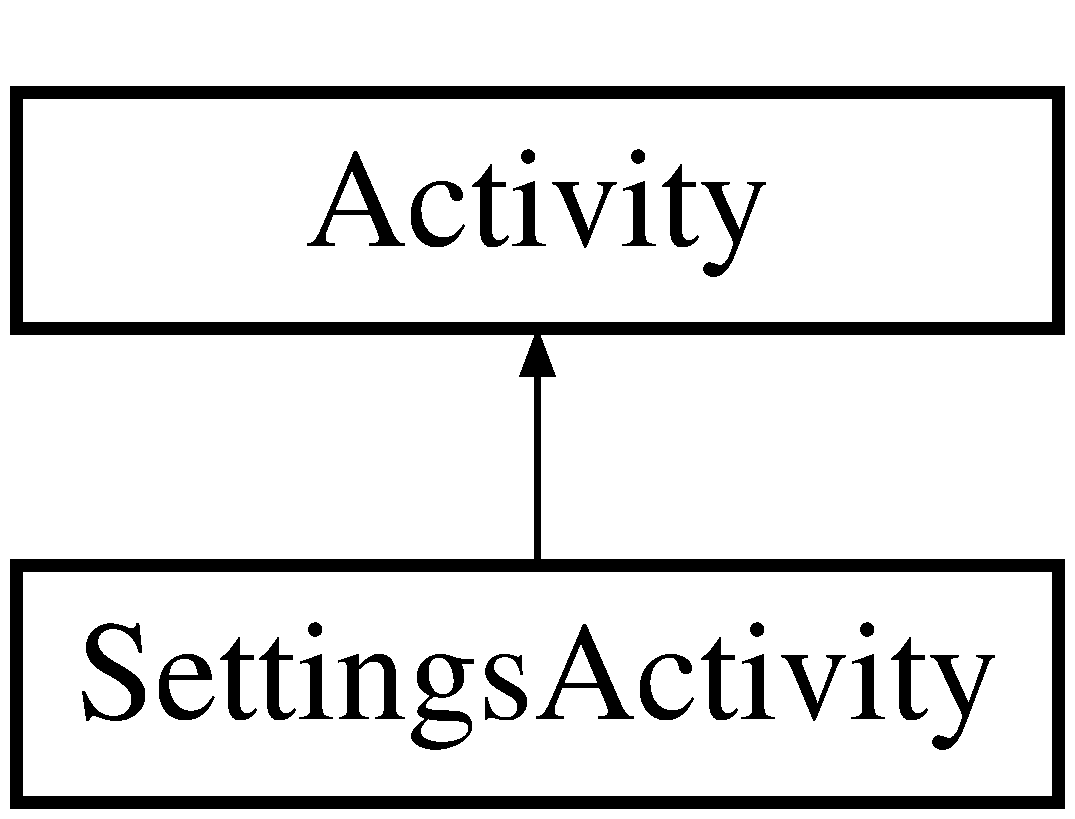
\includegraphics[height=2.000000cm]{classSettingsActivity}
\end{center}
\end{figure}
\subsection*{Public Types}
\begin{DoxyCompactItemize}
\item 
enum {\bfseries Mode} \{ {\bfseries Settings}, 
{\bfseries Language}, 
{\bfseries Sound}
 \}
\end{DoxyCompactItemize}
\subsection*{Public Member Functions}
\begin{DoxyCompactItemize}
\item 
\hypertarget{classSettingsActivity_a2243a5dd63dcda9d28112cfa698ee3a4}{{\bfseries Settings\-Activity} (\hyperlink{classActivity}{Activity} $\ast$parent=N\-U\-L\-L)}\label{classSettingsActivity_a2243a5dd63dcda9d28112cfa698ee3a4}

\item 
\hypertarget{classSettingsActivity_ad4a8a1f8cd88aa8a3e2735a839967d30}{void {\bfseries update} ()}\label{classSettingsActivity_ad4a8a1f8cd88aa8a3e2735a839967d30}

\item 
\hypertarget{classSettingsActivity_a8601d220ba07dfaa166148d46fb7afa5}{void {\bfseries render} ()}\label{classSettingsActivity_a8601d220ba07dfaa166148d46fb7afa5}

\item 
\hypertarget{classSettingsActivity_a11ca3925b64a926011dd4a87645fc8b6}{void {\bfseries mode} (Mode mode)}\label{classSettingsActivity_a11ca3925b64a926011dd4a87645fc8b6}

\end{DoxyCompactItemize}
\subsection*{Additional Inherited Members}


The documentation for this class was generated from the following files\-:\begin{DoxyCompactItemize}
\item 
/home/quentin/\-Projects/\-Asylia/include/activities/Settings\-Activity.\-hpp\item 
/home/quentin/\-Projects/\-Asylia/source/activities/Settings\-Activity.\-cpp\end{DoxyCompactItemize}

\hypertarget{classSkill}{\section{Skill Class Reference}
\label{classSkill}\index{Skill@{Skill}}
}
Inheritance diagram for Skill\-:\begin{figure}[H]
\begin{center}
\leavevmode
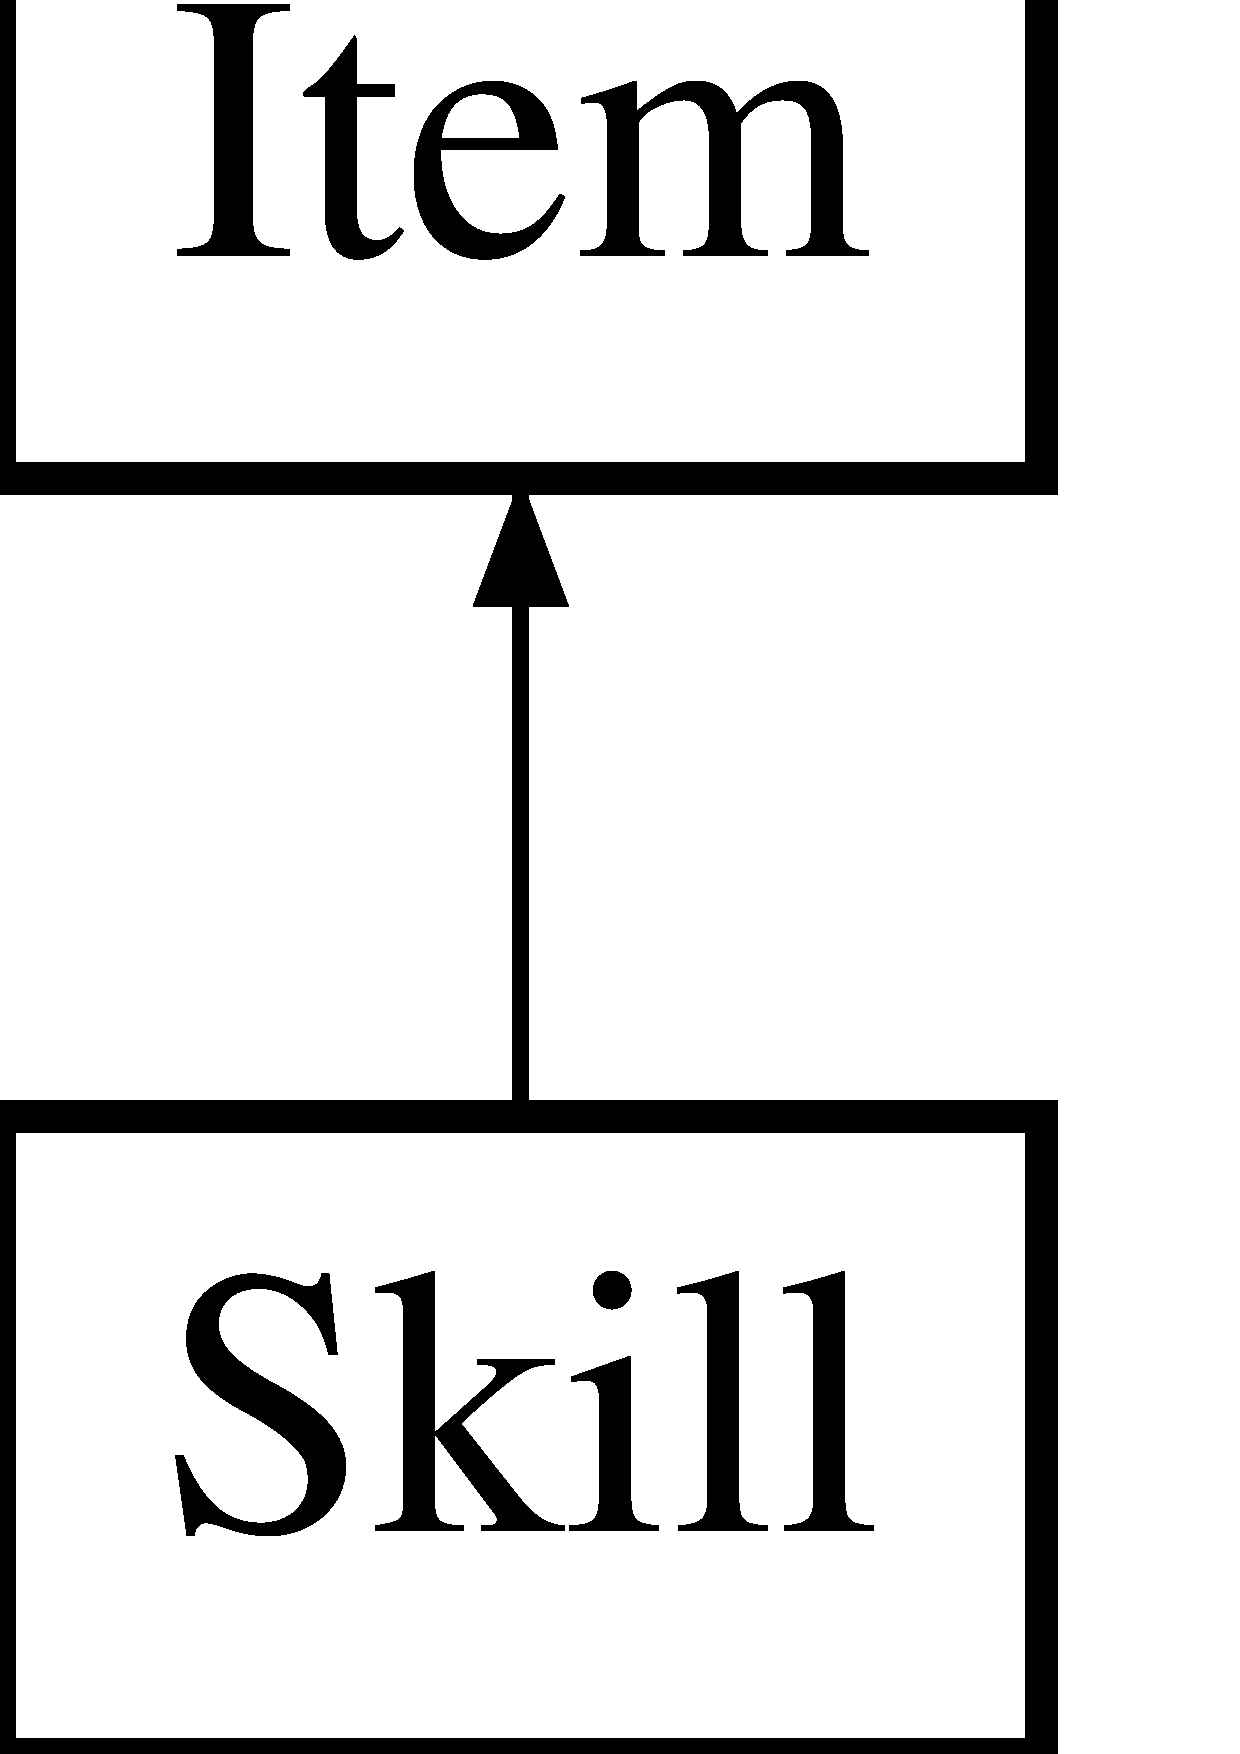
\includegraphics[height=2.000000cm]{classSkill}
\end{center}
\end{figure}
\subsection*{Public Member Functions}
\begin{DoxyCompactItemize}
\item 
\hypertarget{classSkill_a2f4f9de2c5ec6f91f341a60dec4a120b}{{\bfseries Skill} (std\-::string name, std\-::string description, std\-::string thumbnail, \hyperlink{classAnimation}{Animation} $\ast$battle\-Animation, u16 atk, double hit\-Rate)}\label{classSkill_a2f4f9de2c5ec6f91f341a60dec4a120b}

\item 
\hypertarget{classSkill_a05816e34c4fa783e5072a21f18f85a5d}{u16 {\bfseries atk} () const }\label{classSkill_a05816e34c4fa783e5072a21f18f85a5d}

\item 
\hypertarget{classSkill_a34da49de20b937fc79bff950ff4298aa}{double {\bfseries hit\-Rate} () const }\label{classSkill_a34da49de20b937fc79bff950ff4298aa}

\end{DoxyCompactItemize}
\subsection*{Static Public Attributes}
\begin{DoxyCompactItemize}
\item 
\hypertarget{classSkill_a307b7b6a4a71a9aa8a826915dd208dd2}{static u16 {\bfseries count}}\label{classSkill_a307b7b6a4a71a9aa8a826915dd208dd2}

\end{DoxyCompactItemize}
\subsection*{Additional Inherited Members}


The documentation for this class was generated from the following files\-:\begin{DoxyCompactItemize}
\item 
/home/quentin/\-Projects/\-Asylia/include/objects/Skill.\-hpp\item 
/home/quentin/\-Projects/\-Asylia/source/objects/Skill.\-cpp\end{DoxyCompactItemize}

\hypertarget{classSprite}{\section{Sprite Class Reference}
\label{classSprite}\index{Sprite@{Sprite}}
}
Inheritance diagram for Sprite\-:\begin{figure}[H]
\begin{center}
\leavevmode
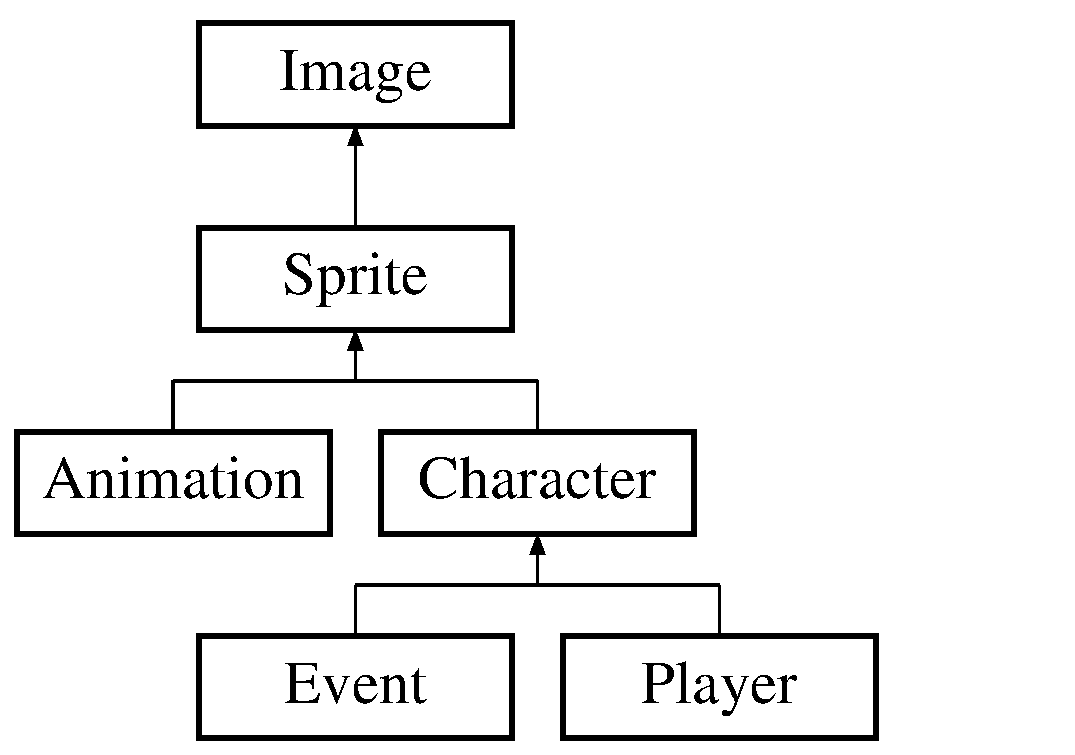
\includegraphics[height=4.000000cm]{classSprite}
\end{center}
\end{figure}
\subsection*{Public Member Functions}
\begin{DoxyCompactItemize}
\item 
\hypertarget{classSprite_a647b6835ac09a05f4a70900209375b20}{{\bfseries Sprite} (const char $\ast$filename, u16 frame\-Width, u16 frame\-Height)}\label{classSprite_a647b6835ac09a05f4a70900209375b20}

\item 
\hypertarget{classSprite_a56c47941d57fc06ea741a89bca10724c}{void {\bfseries reload} (\hyperlink{classSprite}{Sprite} $\ast$sprite)}\label{classSprite_a56c47941d57fc06ea741a89bca10724c}

\item 
\hypertarget{classSprite_ad7562fbe17d1089e427a9068e651052d}{void {\bfseries draw\-Frame} (s16 x, s16 y, u16 frame)}\label{classSprite_ad7562fbe17d1089e427a9068e651052d}

\item 
\hypertarget{classSprite_ad1ed4ec3bf4cf4f53bbf3083a42669a8}{void {\bfseries add\-Animation} (\hyperlink{structSpriteAnimation}{Sprite\-Animation} animation)}\label{classSprite_ad1ed4ec3bf4cf4f53bbf3083a42669a8}

\item 
\hypertarget{classSprite_a096b71a7a19ee192d98184f5660d4aa0}{void {\bfseries reset\-Animation} (u16 anim)}\label{classSprite_a096b71a7a19ee192d98184f5660d4aa0}

\item 
\hypertarget{classSprite_a72dd3f871c8ac44b5460c27f19bda0ea}{void {\bfseries start\-Animation} (u16 anim)}\label{classSprite_a72dd3f871c8ac44b5460c27f19bda0ea}

\item 
\hypertarget{classSprite_a36b49e3976393236c429bdc3ff852fa5}{void {\bfseries stop\-Animation} (u16 anim)}\label{classSprite_a36b49e3976393236c429bdc3ff852fa5}

\item 
\hypertarget{classSprite_a9961ac23adcd7517dc0e385667183b66}{bool {\bfseries animation\-At\-End} (u16 anim)}\label{classSprite_a9961ac23adcd7517dc0e385667183b66}

\item 
\hypertarget{classSprite_af796c0565723dfd94bea0716999fbb83}{bool {\bfseries animation\-At\-Frame} (u16 anim, u16 frame)}\label{classSprite_af796c0565723dfd94bea0716999fbb83}

\item 
\hypertarget{classSprite_a62702abb213905c67227df6ae7ede67b}{void {\bfseries play\-Animation} (s16 x, s16 y, u16 anim)}\label{classSprite_a62702abb213905c67227df6ae7ede67b}

\item 
\hypertarget{classSprite_a354b36eaa7df52728457faf1ccba9d47}{u16 {\bfseries frame\-Width} () const }\label{classSprite_a354b36eaa7df52728457faf1ccba9d47}

\item 
\hypertarget{classSprite_a42620eb04fe4f3e71e351533d5ce9d8b}{u16 {\bfseries frame\-Height} () const }\label{classSprite_a42620eb04fe4f3e71e351533d5ce9d8b}

\item 
\hypertarget{classSprite_a9b414f0f27aa5d62d47fa20c64d800ba}{void {\bfseries set\-Frame\-Size} (u16 width, u16 height)}\label{classSprite_a9b414f0f27aa5d62d47fa20c64d800ba}

\end{DoxyCompactItemize}
\subsection*{Protected Attributes}
\begin{DoxyCompactItemize}
\item 
\hypertarget{classSprite_a165ccf2534677f506b4ae2ea38e988f7}{u16 {\bfseries m\-\_\-frame\-Width}}\label{classSprite_a165ccf2534677f506b4ae2ea38e988f7}

\item 
\hypertarget{classSprite_a9cf36cbf32399c7781bf0bf06d16a7b7}{u16 {\bfseries m\-\_\-frame\-Height}}\label{classSprite_a9cf36cbf32399c7781bf0bf06d16a7b7}

\item 
\hypertarget{classSprite_afed43cbdbec4fbdd8138844384e788ef}{std\-::vector$<$ \hyperlink{structSpriteAnimation}{Sprite\-Animation} $>$ {\bfseries m\-\_\-animations}}\label{classSprite_afed43cbdbec4fbdd8138844384e788ef}

\item 
\hypertarget{classSprite_af082aaf1f64e00cddeed776ff6621fff}{u16 {\bfseries m\-\_\-last\-Frame\-Displayed}}\label{classSprite_af082aaf1f64e00cddeed776ff6621fff}

\end{DoxyCompactItemize}


The documentation for this class was generated from the following files\-:\begin{DoxyCompactItemize}
\item 
/home/quentin/\-Projects/\-Asylia/include/display/Sprite.\-hpp\item 
/home/quentin/\-Projects/\-Asylia/source/display/Sprite.\-cpp\end{DoxyCompactItemize}

\hypertarget{structSpriteAnimation}{\section{Sprite\-Animation Struct Reference}
\label{structSpriteAnimation}\index{Sprite\-Animation@{Sprite\-Animation}}
}
\subsection*{Public Member Functions}
\begin{DoxyCompactItemize}
\item 
\hypertarget{structSpriteAnimation_a714050082b00fdf1fbf7f526c8444422}{{\bfseries Sprite\-Animation} (u16 \-\_\-size, std\-::vector$<$ u16 $>$ \-\_\-tab\-Anim, u16 \-\_\-delay, bool \-\_\-is\-Playing=false)}\label{structSpriteAnimation_a714050082b00fdf1fbf7f526c8444422}

\end{DoxyCompactItemize}
\subsection*{Public Attributes}
\begin{DoxyCompactItemize}
\item 
\hypertarget{structSpriteAnimation_aa547caf0c49262f082865ab9422619ea}{u16 {\bfseries size}}\label{structSpriteAnimation_aa547caf0c49262f082865ab9422619ea}

\item 
\hypertarget{structSpriteAnimation_ab701a6db968f0ded572c40a274947c77}{std\-::vector$<$ u16 $>$ {\bfseries tab\-Anim}}\label{structSpriteAnimation_ab701a6db968f0ded572c40a274947c77}

\item 
\hypertarget{structSpriteAnimation_a8692dae92b2f3f23fb27846fad397f98}{u16 {\bfseries delay}}\label{structSpriteAnimation_a8692dae92b2f3f23fb27846fad397f98}

\item 
\hypertarget{structSpriteAnimation_a7f051b8f289ffd16b226bc2abbd26888}{\hyperlink{classTimer}{Timer} {\bfseries timer}}\label{structSpriteAnimation_a7f051b8f289ffd16b226bc2abbd26888}

\item 
\hypertarget{structSpriteAnimation_a37b4a887ed53f1b808a37dad19083f0e}{bool {\bfseries is\-Playing}}\label{structSpriteAnimation_a37b4a887ed53f1b808a37dad19083f0e}

\end{DoxyCompactItemize}


The documentation for this struct was generated from the following file\-:\begin{DoxyCompactItemize}
\item 
/home/quentin/\-Projects/\-Asylia/include/display/Sprite\-Animation.\-hpp\end{DoxyCompactItemize}

\hypertarget{classStringParameter}{\section{String\-Parameter Class Reference}
\label{classStringParameter}\index{String\-Parameter@{String\-Parameter}}
}
Inheritance diagram for String\-Parameter\-:\begin{figure}[H]
\begin{center}
\leavevmode
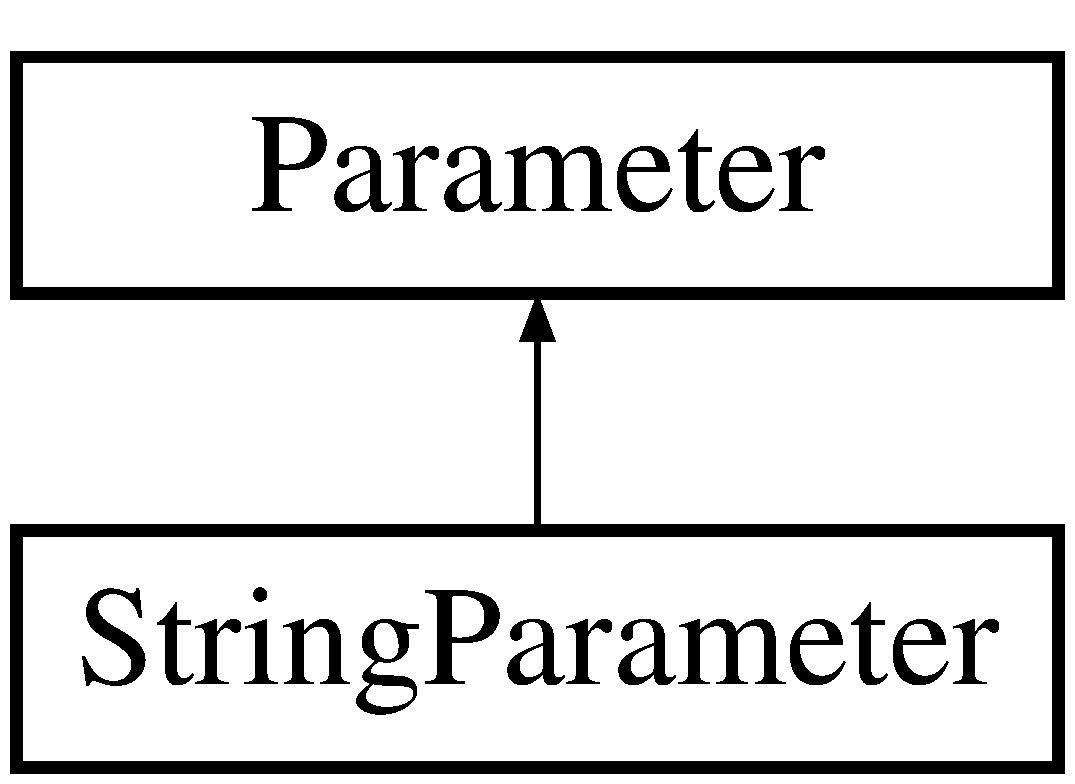
\includegraphics[height=2.000000cm]{classStringParameter}
\end{center}
\end{figure}
\subsection*{Public Member Functions}
\begin{DoxyCompactItemize}
\item 
\hypertarget{classStringParameter_ae33eb047a4bc670d668ec6d42194b107}{{\bfseries String\-Parameter} (std\-::string value)}\label{classStringParameter_ae33eb047a4bc670d668ec6d42194b107}

\item 
\hypertarget{classStringParameter_a0bd5b632da96a3c655fd24e40996b8a8}{void $\ast$ {\bfseries value} ()}\label{classStringParameter_a0bd5b632da96a3c655fd24e40996b8a8}

\end{DoxyCompactItemize}
\subsection*{Additional Inherited Members}


The documentation for this class was generated from the following files\-:\begin{DoxyCompactItemize}
\item 
/home/quentin/\-Projects/\-Asylia/include/core/Parameter.\-hpp\item 
/home/quentin/\-Projects/\-Asylia/source/core/Parameter.\-cpp\end{DoxyCompactItemize}

\hypertarget{classTextWindow}{\section{Text\-Window Class Reference}
\label{classTextWindow}\index{Text\-Window@{Text\-Window}}
}
Inheritance diagram for Text\-Window\-:\begin{figure}[H]
\begin{center}
\leavevmode
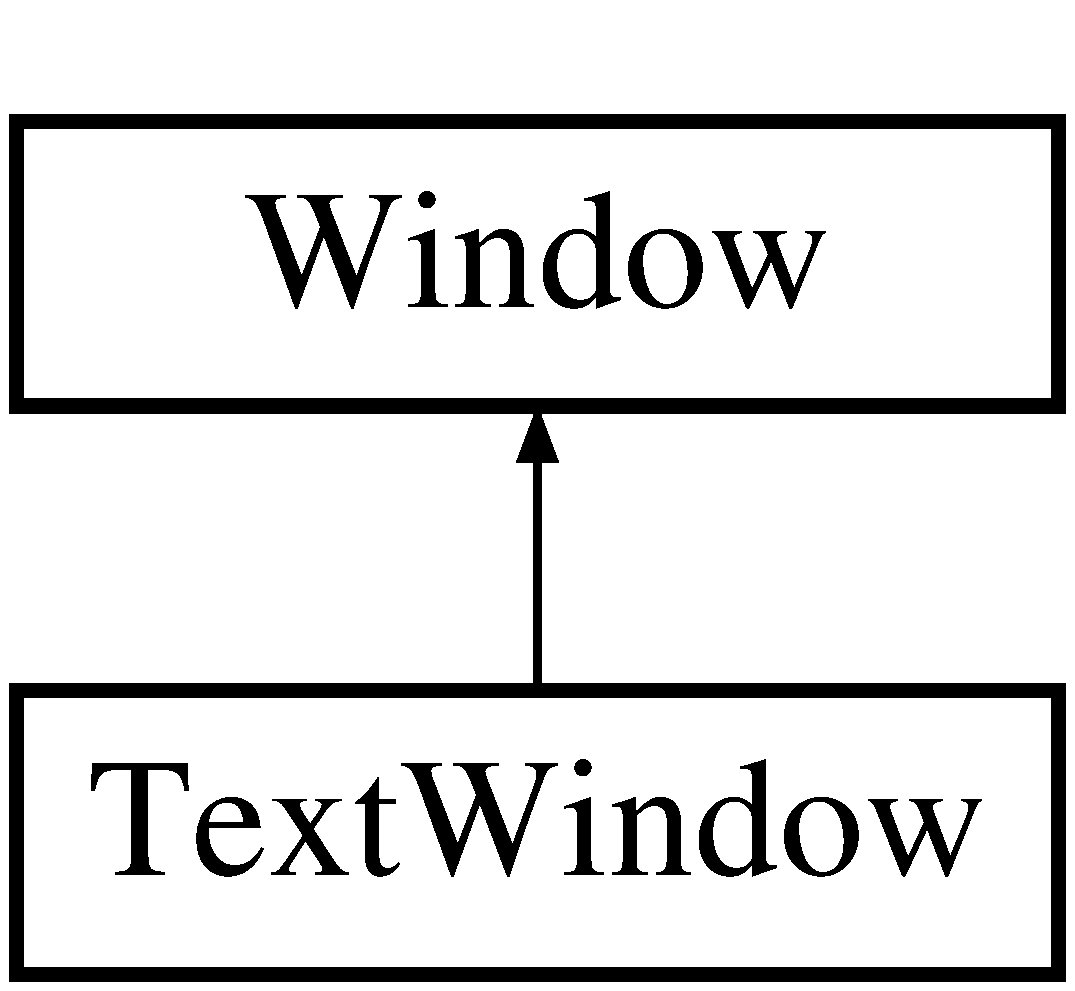
\includegraphics[height=2.000000cm]{classTextWindow}
\end{center}
\end{figure}
\subsection*{Public Member Functions}
\begin{DoxyCompactItemize}
\item 
\hypertarget{classTextWindow_a7f3145cfeeac7765e4e876cefd561754}{{\bfseries Text\-Window} (s16 x, s16 y, u16 width, u16 height)}\label{classTextWindow_a7f3145cfeeac7765e4e876cefd561754}

\item 
\hypertarget{classTextWindow_a47312e546dfbb3de9e87a34c07447985}{void {\bfseries draw} (std\-::string text)}\label{classTextWindow_a47312e546dfbb3de9e87a34c07447985}

\end{DoxyCompactItemize}
\subsection*{Additional Inherited Members}


The documentation for this class was generated from the following files\-:\begin{DoxyCompactItemize}
\item 
/home/quentin/\-Projects/\-Asylia/include/windows/Text\-Window.\-hpp\item 
/home/quentin/\-Projects/\-Asylia/source/windows/Text\-Window.\-cpp\end{DoxyCompactItemize}

\hypertarget{structTileset}{\section{Tileset Struct Reference}
\label{structTileset}\index{Tileset@{Tileset}}
}
\subsection*{Public Attributes}
\begin{DoxyCompactItemize}
\item 
\hypertarget{structTileset_ad4b0634b055591c2f4a50104fe72eef6}{\hyperlink{classImage}{Image} $\ast$ {\bfseries tiles}}\label{structTileset_ad4b0634b055591c2f4a50104fe72eef6}

\item 
\hypertarget{structTileset_a06c3121f06b5543f9f4d57c6297aeb23}{u16 {\bfseries tile\-Width}}\label{structTileset_a06c3121f06b5543f9f4d57c6297aeb23}

\item 
\hypertarget{structTileset_ac83b45e8d0ebb54ae8ac014715ce166b}{u16 {\bfseries tile\-Height}}\label{structTileset_ac83b45e8d0ebb54ae8ac014715ce166b}

\item 
\hypertarget{structTileset_a8119ef6379c624f361a5929ec5a6a1d9}{u16 $\ast$ {\bfseries non\-Passable\-Layer}}\label{structTileset_a8119ef6379c624f361a5929ec5a6a1d9}

\end{DoxyCompactItemize}


The documentation for this struct was generated from the following file\-:\begin{DoxyCompactItemize}
\item 
/home/quentin/\-Projects/\-Asylia/include/display/Tileset.\-hpp\end{DoxyCompactItemize}

\hypertarget{classTimer}{\section{Timer Class Reference}
\label{classTimer}\index{Timer@{Timer}}
}
\subsection*{Public Member Functions}
\begin{DoxyCompactItemize}
\item 
\hypertarget{classTimer_a63f0eb44b27402196590a03781515dba}{void {\bfseries stop} ()}\label{classTimer_a63f0eb44b27402196590a03781515dba}

\item 
\hypertarget{classTimer_a3a8b5272198d029779dc9302a54305a8}{void {\bfseries start} ()}\label{classTimer_a3a8b5272198d029779dc9302a54305a8}

\item 
\hypertarget{classTimer_a9020542d73357a4eef512eefaf57524b}{void {\bfseries reset} ()}\label{classTimer_a9020542d73357a4eef512eefaf57524b}

\item 
\hypertarget{classTimer_a3d9d0ccaf75f0d3f797a8db267d0a7bb}{bool {\bfseries is\-Started} () const }\label{classTimer_a3d9d0ccaf75f0d3f797a8db267d0a7bb}

\item 
\hypertarget{classTimer_a250547797fd2a49df2f2b5f1667ddc79}{u16 {\bfseries time} ()}\label{classTimer_a250547797fd2a49df2f2b5f1667ddc79}

\end{DoxyCompactItemize}


The documentation for this class was generated from the following files\-:\begin{DoxyCompactItemize}
\item 
/home/quentin/\-Projects/\-Asylia/include/display/Timer.\-hpp\item 
/home/quentin/\-Projects/\-Asylia/source/display/Timer.\-cpp\end{DoxyCompactItemize}

\hypertarget{classTitleActivity}{\section{Title\-Activity Class Reference}
\label{classTitleActivity}\index{Title\-Activity@{Title\-Activity}}
}
Inheritance diagram for Title\-Activity\-:\begin{figure}[H]
\begin{center}
\leavevmode
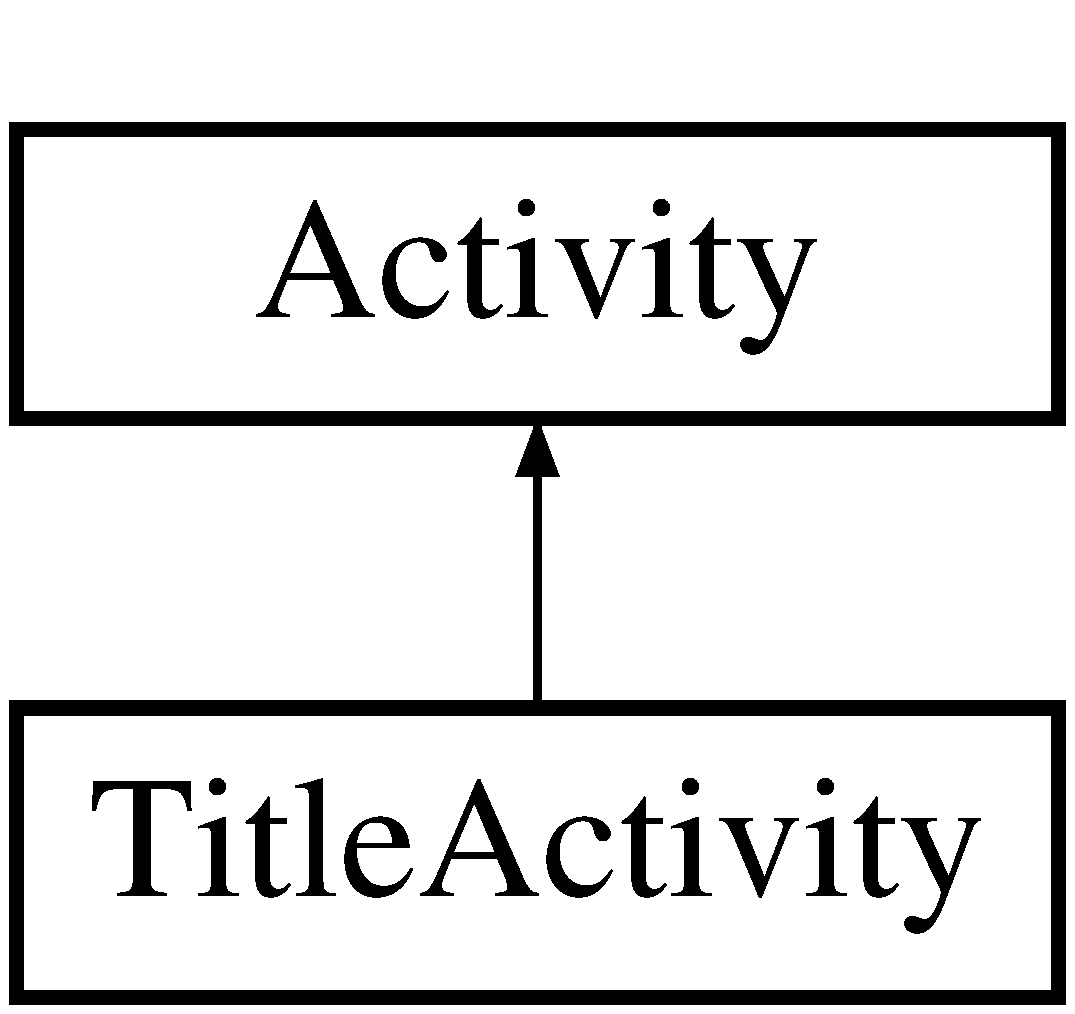
\includegraphics[height=2.000000cm]{classTitleActivity}
\end{center}
\end{figure}
\subsection*{Public Member Functions}
\begin{DoxyCompactItemize}
\item 
\hypertarget{classTitleActivity_a80c9fdc0811304a023b1ae19ee2e0b9f}{void {\bfseries update} ()}\label{classTitleActivity_a80c9fdc0811304a023b1ae19ee2e0b9f}

\item 
\hypertarget{classTitleActivity_af8800c5968935fbb710da6ea7a0e5e9f}{void {\bfseries render} ()}\label{classTitleActivity_af8800c5968935fbb710da6ea7a0e5e9f}

\end{DoxyCompactItemize}
\subsection*{Additional Inherited Members}


The documentation for this class was generated from the following files\-:\begin{DoxyCompactItemize}
\item 
/home/quentin/\-Projects/\-Asylia/include/activities/Title\-Activity.\-hpp\item 
/home/quentin/\-Projects/\-Asylia/source/activities/Title\-Activity.\-cpp\end{DoxyCompactItemize}

\hypertarget{classTroop}{\section{Troop Class Reference}
\label{classTroop}\index{Troop@{Troop}}
}
\subsection*{Public Member Functions}
\begin{DoxyCompactItemize}
\item 
\hypertarget{classTroop_ae8c6302f0c441f2705cc479f6bef01a2}{{\bfseries Troop} (\hyperlink{classImage}{Image} $\ast$battleback=N\-U\-L\-L)}\label{classTroop_ae8c6302f0c441f2705cc479f6bef01a2}

\item 
\hypertarget{classTroop_ad747c6ae6caa4013d05835db28858c7b}{\hyperlink{classImage}{Image} $\ast$ {\bfseries battleback} () const }\label{classTroop_ad747c6ae6caa4013d05835db28858c7b}

\item 
\hypertarget{classTroop_a931da8e3b88bbd755bb1d7e636b76330}{void {\bfseries add\-Enemy} (\hyperlink{classEnemy}{Enemy} $\ast$enemy, s16 x, s16 y)}\label{classTroop_a931da8e3b88bbd755bb1d7e636b76330}

\item 
\hypertarget{classTroop_a425971336ea0a55c4fe19ffdabaa1e5a}{\hyperlink{classEnemy}{Enemy} $\ast$ {\bfseries get\-Enemy} (u8 pos)}\label{classTroop_a425971336ea0a55c4fe19ffdabaa1e5a}

\item 
\hypertarget{classTroop_a79e2700df4e1628351ff2f19c7d37545}{s16 {\bfseries get\-Enemy\-X} (u8 pos)}\label{classTroop_a79e2700df4e1628351ff2f19c7d37545}

\item 
\hypertarget{classTroop_ad09bc365656cef0efc4fe34f0e4a0d30}{s16 {\bfseries get\-Enemy\-Y} (u8 pos)}\label{classTroop_ad09bc365656cef0efc4fe34f0e4a0d30}

\item 
\hypertarget{classTroop_a7ff2cb2e7cf34acd7ba8c286b2d87c62}{u8 {\bfseries size} ()}\label{classTroop_a7ff2cb2e7cf34acd7ba8c286b2d87c62}

\end{DoxyCompactItemize}


The documentation for this class was generated from the following files\-:\begin{DoxyCompactItemize}
\item 
/home/quentin/\-Projects/\-Asylia/include/objects/Troop.\-hpp\item 
/home/quentin/\-Projects/\-Asylia/source/objects/Troop.\-cpp\end{DoxyCompactItemize}

\hypertarget{classVictoryWindow}{\section{Victory\-Window Class Reference}
\label{classVictoryWindow}\index{Victory\-Window@{Victory\-Window}}
}
Inheritance diagram for Victory\-Window\-:\begin{figure}[H]
\begin{center}
\leavevmode
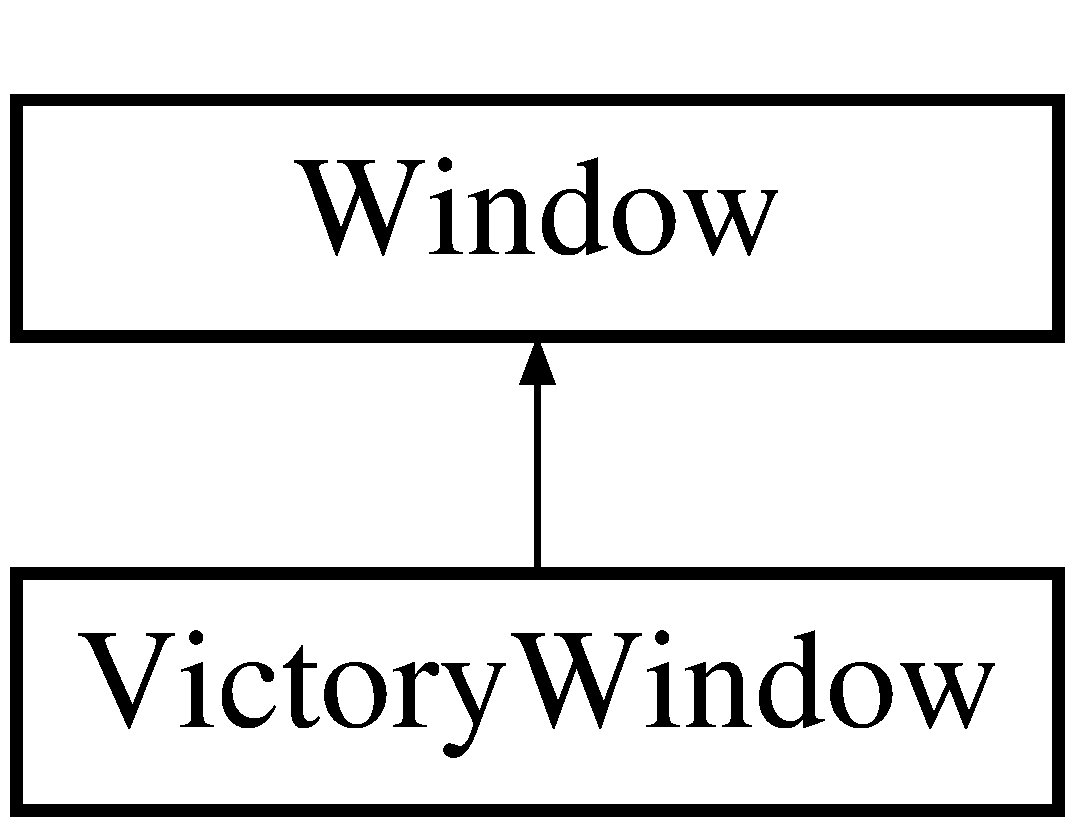
\includegraphics[height=2.000000cm]{classVictoryWindow}
\end{center}
\end{figure}
\subsection*{Public Member Functions}
\begin{DoxyCompactItemize}
\item 
\hypertarget{classVictoryWindow_a5f3da410bd0dbb63afba25aadea6222d}{{\bfseries Victory\-Window} (\hyperlink{classBattle}{Battle} $\ast$battle)}\label{classVictoryWindow_a5f3da410bd0dbb63afba25aadea6222d}

\item 
\hypertarget{classVictoryWindow_a6eef42e3d15f12aa872fa77b145150ac}{void {\bfseries draw} ()}\label{classVictoryWindow_a6eef42e3d15f12aa872fa77b145150ac}

\end{DoxyCompactItemize}
\subsection*{Additional Inherited Members}


The documentation for this class was generated from the following files\-:\begin{DoxyCompactItemize}
\item 
/home/quentin/\-Projects/\-Asylia/include/windows/Victory\-Window.\-hpp\item 
/home/quentin/\-Projects/\-Asylia/source/windows/Victory\-Window.\-cpp\end{DoxyCompactItemize}

\hypertarget{classWeapon}{\section{Weapon Class Reference}
\label{classWeapon}\index{Weapon@{Weapon}}
}
Inheritance diagram for Weapon\-:\begin{figure}[H]
\begin{center}
\leavevmode
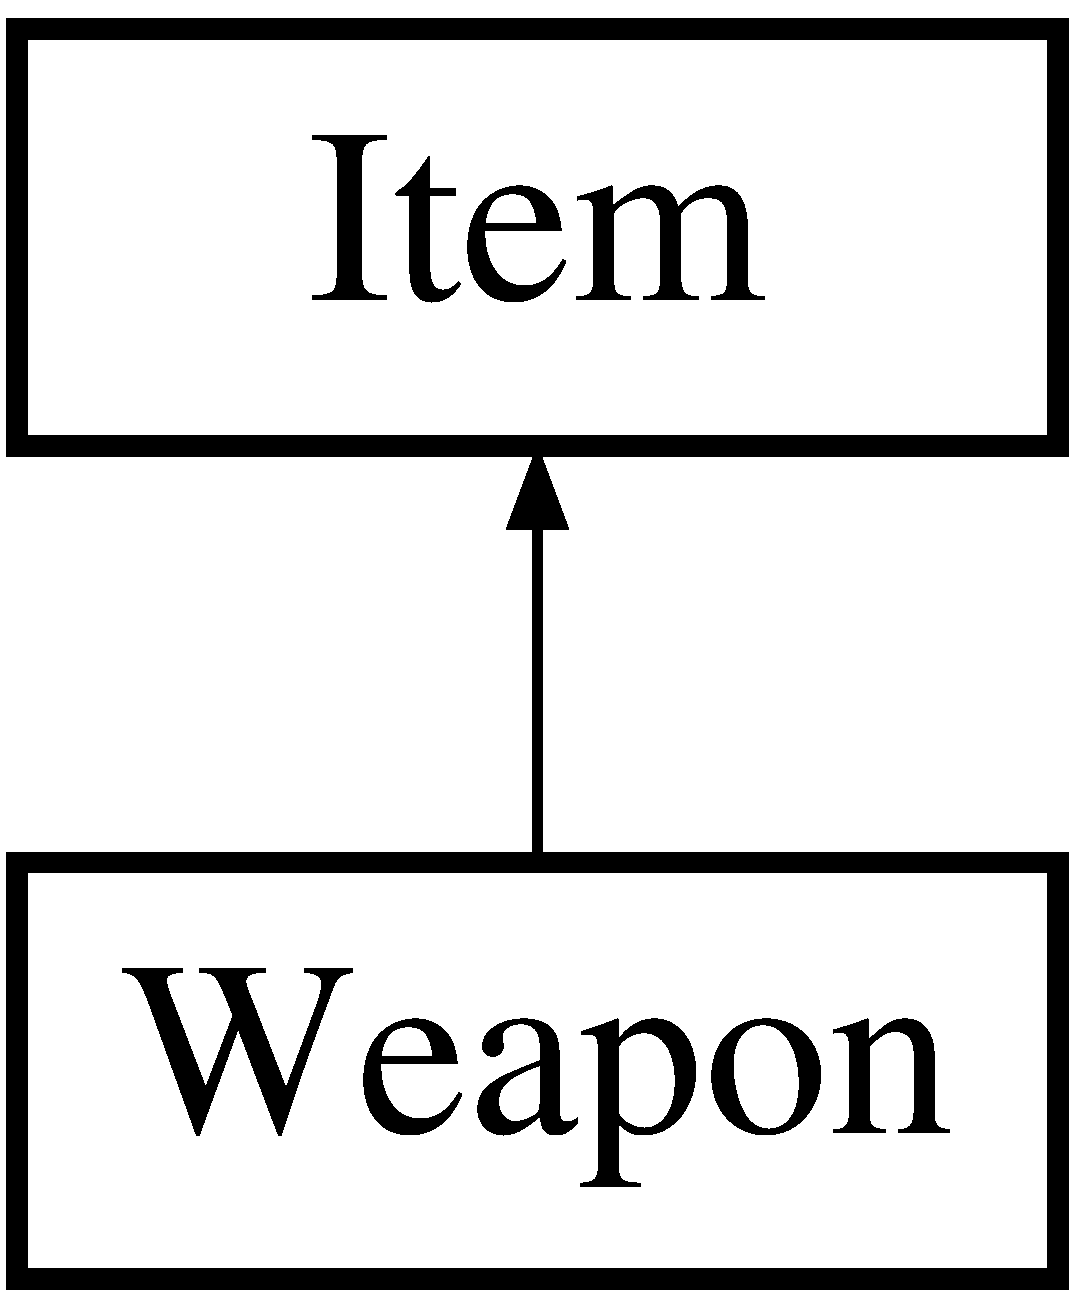
\includegraphics[height=2.000000cm]{classWeapon}
\end{center}
\end{figure}
\subsection*{Public Member Functions}
\begin{DoxyCompactItemize}
\item 
\hypertarget{classWeapon_aa7ec72341a8f3f6f8a21129ff1f330d2}{{\bfseries Weapon} (std\-::string name, std\-::string description, std\-::string thumbnail, u16 atk, double hit\-Rate)}\label{classWeapon_aa7ec72341a8f3f6f8a21129ff1f330d2}

\item 
\hypertarget{classWeapon_a634ac28e7909b7e99075299e51ff178e}{u16 {\bfseries atk} () const }\label{classWeapon_a634ac28e7909b7e99075299e51ff178e}

\item 
\hypertarget{classWeapon_ad13d6e681b6698cdcb493e426d9fc740}{double {\bfseries hit\-Rate} () const }\label{classWeapon_ad13d6e681b6698cdcb493e426d9fc740}

\item 
\hypertarget{classWeapon_ae4fc252e5bc48bb8c4bb492f751bd963}{u8 {\bfseries equip\-Type} () const }\label{classWeapon_ae4fc252e5bc48bb8c4bb492f751bd963}

\end{DoxyCompactItemize}
\subsection*{Additional Inherited Members}


The documentation for this class was generated from the following files\-:\begin{DoxyCompactItemize}
\item 
/home/quentin/\-Projects/\-Asylia/include/objects/Weapon.\-hpp\item 
/home/quentin/\-Projects/\-Asylia/source/objects/Weapon.\-cpp\end{DoxyCompactItemize}

\hypertarget{classWindow}{\section{Window Class Reference}
\label{classWindow}\index{Window@{Window}}
}
Inheritance diagram for Window\-:\begin{figure}[H]
\begin{center}
\leavevmode
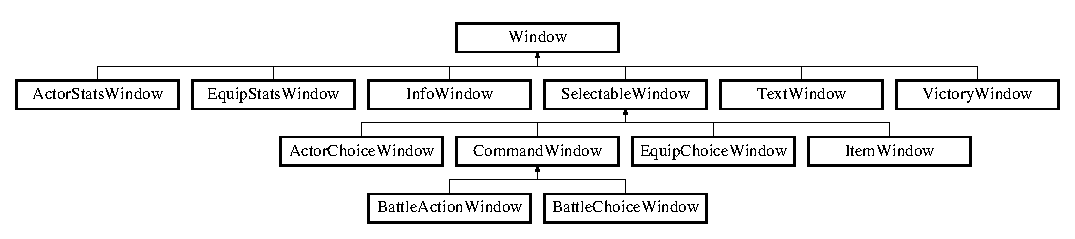
\includegraphics[height=2.765432cm]{classWindow}
\end{center}
\end{figure}
\subsection*{Public Member Functions}
\begin{DoxyCompactItemize}
\item 
\hypertarget{classWindow_a8a34ab9865729e9075acc3e0a99f121b}{{\bfseries Window} (s16 x, s16 y, u16 width, u16 height)}\label{classWindow_a8a34ab9865729e9075acc3e0a99f121b}

\item 
\hypertarget{classWindow_a59515fc5a56e86d5a46d771595daac55}{void {\bfseries update} ()}\label{classWindow_a59515fc5a56e86d5a46d771595daac55}

\item 
\hypertarget{classWindow_a05e89849f1b82b2f47c7428e4145ad6c}{void {\bfseries draw\-Cursor} (s16 x, s16 y, u16 width, u16 height)}\label{classWindow_a05e89849f1b82b2f47c7428e4145ad6c}

\item 
\hypertarget{classWindow_a6a1e38ec09e8a262e485c49475840bcb}{void {\bfseries draw} (bool cursor=true)}\label{classWindow_a6a1e38ec09e8a262e485c49475840bcb}

\item 
\hypertarget{classWindow_ae9a1f20119b4633e29931593e8c76a4e}{s16 {\bfseries x} () const }\label{classWindow_ae9a1f20119b4633e29931593e8c76a4e}

\item 
\hypertarget{classWindow_a2018bb6253b2e1357b90e6aaadcece21}{s16 {\bfseries y} () const }\label{classWindow_a2018bb6253b2e1357b90e6aaadcece21}

\item 
\hypertarget{classWindow_a1a14b80d65c1a9824bf623880f2fbaad}{u16 {\bfseries width} () const }\label{classWindow_a1a14b80d65c1a9824bf623880f2fbaad}

\item 
\hypertarget{classWindow_aaf54b86cda72283958fba3f904ed5f6d}{u16 {\bfseries height} () const }\label{classWindow_aaf54b86cda72283958fba3f904ed5f6d}

\item 
\hypertarget{classWindow_a2c720225fd60f19cfe046e764978c8f8}{void {\bfseries x} (s16 x)}\label{classWindow_a2c720225fd60f19cfe046e764978c8f8}

\item 
\hypertarget{classWindow_a7166a3e1101ebc1d6e2d9817eec2857b}{void {\bfseries y} (s16 y)}\label{classWindow_a7166a3e1101ebc1d6e2d9817eec2857b}

\item 
\hypertarget{classWindow_a1d8354a03f5fd148aeebc83c9602a5c9}{void {\bfseries width} (u16 width)}\label{classWindow_a1d8354a03f5fd148aeebc83c9602a5c9}

\item 
\hypertarget{classWindow_a071e45e1e861b032444a078a7241c70b}{void {\bfseries height} (u16 height)}\label{classWindow_a071e45e1e861b032444a078a7241c70b}

\item 
\hypertarget{classWindow_a1c3093631aa79c6038f86b7dc511553c}{void {\bfseries print\-Stat} (s16 x, s16 y, std\-::string stat\-Name, s32 stat\-Value, u16 name\-Width, u16 width, u16 max=0)}\label{classWindow_a1c3093631aa79c6038f86b7dc511553c}

\item 
\hypertarget{classWindow_a4a7493ad69c93233c28a0e1e66b327e3}{void {\bfseries print\-Name} (\hyperlink{classBattler}{Battler} $\ast$battler, s16 x, s16 y, u16 width)}\label{classWindow_a4a7493ad69c93233c28a0e1e66b327e3}

\item 
\hypertarget{classWindow_a5489ce4a2eab4a930d94f852cbba8ee5}{void {\bfseries print\-State} (\hyperlink{classBattler}{Battler} $\ast$battler, s16 x, s16 y, u16 width)}\label{classWindow_a5489ce4a2eab4a930d94f852cbba8ee5}

\item 
\hypertarget{classWindow_a4662dbf66c08dfefcb0a891969235fbf}{void {\bfseries print\-Level} (\hyperlink{classBattler}{Battler} $\ast$battler, s16 x, s16 y, s16 x2)}\label{classWindow_a4662dbf66c08dfefcb0a891969235fbf}

\item 
\hypertarget{classWindow_a63acc98030cfcfa877ffe76b264b7590}{void {\bfseries print\-H\-P} (\hyperlink{classBattler}{Battler} $\ast$battler, s16 x, s16 y, s16 x2, bool on\-Maximum=false)}\label{classWindow_a63acc98030cfcfa877ffe76b264b7590}

\item 
\hypertarget{classWindow_a8d8cf8c7d7450ff5c54f8050d9757463}{void {\bfseries print\-S\-P} (\hyperlink{classBattler}{Battler} $\ast$battler, s16 x, s16 y, s16 x2, bool on\-Maximum=false)}\label{classWindow_a8d8cf8c7d7450ff5c54f8050d9757463}

\item 
\hypertarget{classWindow_a90b7b925030c07f9d26ac5eb1e2ac54a}{void {\bfseries print\-Exp} (\hyperlink{classBattler}{Battler} $\ast$battler, s16 x, s16 y, s16 x2, bool on\-Maximum=false)}\label{classWindow_a90b7b925030c07f9d26ac5eb1e2ac54a}

\item 
\hypertarget{classWindow_a1faf3d8d1315aff937ff83ca7a7c0e51}{void {\bfseries draw\-Battler} (\hyperlink{classBattler}{Battler} $\ast$battler, s16 x, s16 y)}\label{classWindow_a1faf3d8d1315aff937ff83ca7a7c0e51}

\item 
\hypertarget{classWindow_aef2352043900c81f90b9c8bde9b509bf}{void {\bfseries print\-Item} (\hyperlink{classItem}{Item} $\ast$item, u16 count, s16 x, s16 y, u16 width)}\label{classWindow_aef2352043900c81f90b9c8bde9b509bf}

\end{DoxyCompactItemize}
\subsection*{Protected Attributes}
\begin{DoxyCompactItemize}
\item 
\hypertarget{classWindow_a9c81381f61395db2cd2a29d4bcd73c40}{s16 {\bfseries m\-\_\-x}}\label{classWindow_a9c81381f61395db2cd2a29d4bcd73c40}

\item 
\hypertarget{classWindow_aed13dcbadd684012cb454f0ddf95b938}{s16 {\bfseries m\-\_\-y}}\label{classWindow_aed13dcbadd684012cb454f0ddf95b938}

\item 
\hypertarget{classWindow_a28cc4474674225a826c0b97df1c1fbda}{u16 {\bfseries m\-\_\-width}}\label{classWindow_a28cc4474674225a826c0b97df1c1fbda}

\item 
\hypertarget{classWindow_a0ebb6c7563f270290663b3c79aeffe70}{u16 {\bfseries m\-\_\-height}}\label{classWindow_a0ebb6c7563f270290663b3c79aeffe70}

\item 
\hypertarget{classWindow_a298b2bc9476a79142f5a2aed7a7b526c}{\hyperlink{structRectangle}{Rectangle} {\bfseries m\-\_\-cursor}}\label{classWindow_a298b2bc9476a79142f5a2aed7a7b526c}

\end{DoxyCompactItemize}


The documentation for this class was generated from the following files\-:\begin{DoxyCompactItemize}
\item 
/home/quentin/\-Projects/\-Asylia/include/windows/Window.\-hpp\item 
/home/quentin/\-Projects/\-Asylia/source/windows/Window.\-cpp\end{DoxyCompactItemize}

\hypertarget{classXMLFile}{\section{X\-M\-L\-File Class Reference}
\label{classXMLFile}\index{X\-M\-L\-File@{X\-M\-L\-File}}
}
\subsection*{Public Member Functions}
\begin{DoxyCompactItemize}
\item 
\hypertarget{classXMLFile_a3f6ee539d05eace7843006da01e33e53}{{\bfseries X\-M\-L\-File} (const char $\ast$filename)}\label{classXMLFile_a3f6ee539d05eace7843006da01e33e53}

\item 
\hypertarget{classXMLFile_adc30aaf5a1cecc72ed8846d0907b48e6}{X\-M\-L\-Handle {\bfseries First\-Child\-Element} (const char $\ast$element)}\label{classXMLFile_adc30aaf5a1cecc72ed8846d0907b48e6}

\end{DoxyCompactItemize}


The documentation for this class was generated from the following files\-:\begin{DoxyCompactItemize}
\item 
/home/quentin/\-Projects/\-Asylia/include/core/X\-M\-L\-File.\-hpp\item 
/home/quentin/\-Projects/\-Asylia/source/core/X\-M\-L\-File.\-cpp\end{DoxyCompactItemize}

%--- End generated contents ---

% Index
\newpage
\phantomsection
\addcontentsline{toc}{chapter}{Index}
\printindex

\end{document}
